% !TEX root =  lectures.tex
\documentclass[12pt]{article}
\usepackage{graphicx}
\usepackage[
	pdfencoding=auto,%
	pdftitle={PHY 321, Classical Mechanics I, Lecture Notes},%
	pdfauthor={Scott Pratt},%
	pdfstartview=FitV,%
	colorlinks=true,%
	linkcolor=blue,%
	citecolor=black, %
	urlcolor=blue]{hyperref}
%\usepackage{pdfsync}
\usepackage{amssymb}
\usepackage{amsmath}
\usepackage{bm}
\usepackage{bbold}
\numberwithin{equation}{section} 
\numberwithin{figure}{section} 
\usepackage[small,bf]{caption}

\usepackage{fontspec}
\usepackage{textcomp}
\usepackage{graphicx}
\usepackage{color}
\usepackage{fancyhdr}
\usepackage{bm}

\newcounter{examplecounter}
\setcounter{examplecounter}{0}
\newcommand{\example}{
\stepcounter{examplecounter}{\nopagebreak\noindent\rule{\textwidth}{1pt}\nopagebreak\\ \bf Example \nopagebreak \arabic{section}.\arabic{examplecounter}:\\ \nopagebreak}}

\newcommand{\exampleend}{
\begin{samepage}
\nopagebreak\noindent\rule{\textwidth}{1pt}
\end{samepage}}

%\usepackage[T1]{fontenc}
%\renewcommand*{\sfdefault}{Berenis}
%\renewcommand*{\rmdefault}{Berenis}
%\renewcommand*{\sfdefault}{phv} % helvetica
%\renewcommand*{\sfdefault}{ppl} % palatino
%\renewcommand*{\rmdefault}{ppl}
%\renewcommand*{\sfdefault}{Bookman}
%\renewcommand*{\rmdefault}{Bookman}

\defaultfontfeatures{Scale=MatchLowercase}
%\setmainfont[Mapping=tex-text,SmallCapsFont={CalifornianFB Expert}]{CalifornianFB}
%\setmainfont[Mapping=tex-text]{Minion Pro}
\setmainfont[Mapping=tex-text]{Palatino Bold}
\setmonofont[Mapping=tex-text]{Courier New Bold}
%\setsansfont[Mapping=tex-text]{Myriad Pro}
%\usepackage{xltxtra}
%\setromanfont{Palatino}
\setromanfont{Palatino Bold}


%\pagestyle{empty}
\textwidth 7.0in
\hoffset -0.8in
\textheight 9.4in
\voffset -1in

\pagestyle{fancy}             % page layout
\newcommand{\TheShortTitle}{}
\newcommand{\ShortTitle}[1]{\renewcommand{\TheShortTitle}{#1}}
\fancyhead[LO,RE]{\slshape \TheShortTitle}
\fancyhead[LE,RO]{\slshape \leftmark}

\usepackage{colortbl}
\newcommand{\cc}[1]{\cellcolor{#1}}
\definecolor{lightred}{rgb}{1,0.5,0.6}
\definecolor{lightblue}{rgb}{0.6,0.8,1.0}

\usepackage{comment}
\parskip 4pt
\parindent 0pt

%\newcommand{\bm}{\boldmath}
\boldmath

% for the banner across the tops of pages 2-
\ShortTitle{PHY 831}

\ShortTitle{PHY 321 Lecture Notes}



% for the banner across the tops of pages 2-


\begin{document}

\pagestyle{empty}

% front matter
\centerline{\Large Lecture Notes}

\bigskip

\centerline{\it\Large PHY 321 - Classical Mechanics I}

\centerline{\href{http://www.pa.msu.edu/people/pratts/phy321}{http://www.pa.msu.edu/people/pratts/phy321}}
\medskip
\centerline{\large Instructor: Scott Pratt, prattsc@msu.edu}


\medskip

These notes are {\bf NOT} meant to be a substitute for the book. The text \href{http://www.amazon.com/Classical-Mechanics-John-R-Taylor/dp/189138922X}{Classical Mechanics} by John R. Taylor is required. The course will follow the order of material in the text. These notes are only meant to outline what was covered in class and to provide something students can print and annotate rather than taking full lecture notes.

\tableofcontents

\newpage

\pagestyle{fancy}

\setcounter{page}{1} 
\setcounter{section}{0}

\setcounter{examplecounter}{0}
% !TEX root = lectures.tex
\section{Math Basics}
\bigskip

\subsection{Scalars, Vectors and Matrices}

A scalar is something with a value that is independent of coordinate system. Examples are mass, or the relative time between events. A vector has magnitude and direction. Under rotation, the magnitude stays the same but the direction changes. Scalars have no spatial index, whereas a three-dimensional vector has 3 indices, e.g. the position $\vec{r}$ has components $r_1,r_2,r_3$, which are often referred to as $x,y,z$.

There are several categories of changes of coordinate system. The observer can translate the origin, might move with a different velocity, or might rotate his/her coordinate axes. For instance, a particle's position vector changes when the origin is translated, but its velocity does not. When you study relativity you will find that quantities you thought of as scalars, such as time or electric potential, are actually parts of four-dimensional vectors and that changes of the velocity of the reference frame act in a similar way to rotations.

In addition to vectors and scalars, there are matrices, which have two indices. One also has objects with 3 or four indices. These are called tensors of rank $n$, where $n$ is the number of indices. A matrix is a rank-two tensor. The Levi-Civita symbol, $\epsilon_{ijk}$ used for cross products, is a third-rank tensor.

\subsubsection*{Unit Vectors}

Also known as basis vectors, unit vectors point in the direction of the coordinate axes, have unit norm, and are orthogonal to one another. Sometimes this is referred to as an orthonormal basis,
\begin{equation}
\hat{e}_i\cdot\hat{e}_j=\delta_{ij}=\left(\begin{array}{ccc}
1 & 0 & 0\\
0& 1 & 0\\
0 & 0 & 1
\end{array}\right).
\end{equation}
Here, $\delta_{ij}$ is unity when $i=j$ and is zero otherwise. This is called the unit matrix, because you can multiply it with any other matrix and not change the matrix. The ``dot'' denotes the dot product, $\vec{A}\cdot\vec{B}=A_1B_1+A_2B_2+A_3B_3=|A||B|\cos\theta_{AB}$. Sometimes the unit vectors are called $\hat{x}$, $\hat{y}$ and $\hat{z}$. Vectors can be decomposed in terms of unit vectors,
\begin{equation}
\vec{r}=r_1\hat{e}_1+r_2\hat{e}_2+r_3\hat{e}_3.
\end{equation}
The vector components $r_1$, $r_2$ and $r_3$ might be called $x$, $y$ and $z$ for a displacement of $v_x$, $v_y$ and $v_z$ for a velocity.

\subsubsection*{Rotations}

Here, we use rotations as an example of matrices and their operations. One can consider a different orthonormal basis $\hat{e}'_1$, $\hat{e}'_2$ and $\hat{e}'_3$. The same vector $\vec{r}$ mentioned above can also be expressed in the new basis,
\begin{equation}
\vec{r}=r'_1\hat{e}'_1+r'_2\hat{e}'_2+r'_3\hat{e}'_3.
\end{equation}
Even though it is the same vector, the components have changed. Each new unit vector $\hat{e}'_i$ can be expressed as a linear sum of the previous vectors,
\begin{equation}
\hat{e}'_i=\sum_j U_{ij}\hat{e}_j,
\end{equation}
and the matrix $U$ can be found by taking the dot product of both sides with $\hat{e}_k$,
\begin{eqnarray}
\nonumber
\hat{e}_k\cdot\hat{e}'_i&=&\sum_jU_{ij}\hat{e}_k\cdot\hat{e}_j\\
\label{eq:lambda_angles}
\hat{e}_k\cdot\hat{e}'_i&=&\sum_jU_{ij}\delta_{jk}=U_{ik}.
\end{eqnarray}
Thus, the matrix lambda has components $U_{ij}$ that are equal to the cosine of the angle between new unit vector $\hat{e}'_i$ and the old unit vector $\hat{e}_j$.
\begin{equation}
U = \left(\begin{array}{ccc}
\hat{e}'_1\cdot\hat{e}_1& \hat{e}'_1\cdot\hat{e}_2& \hat{e}'_1\cdot\hat{e}_3\\
\hat{e}'_2\cdot\hat{e}_1& \hat{e}'_2\cdot\hat{e}_2& \hat{e}'_2\cdot\hat{e}_3\\
\hat{e}'_3\cdot\hat{e}_1& \hat{e}'_3\cdot\hat{e}_2& \hat{e}'_3\cdot\hat{e}_3
\end{array}\right),~~~~~U_{ij}=\hat{e}'_i\cdot\hat{e}_j=\cos\theta_{ij}.
\end{equation}
Note that the matrix is not symmetric, $U_{ij}\ne U_{ji}$. One can also look at the inverse transformation, by switching the primed and unprimed coordinates,
\begin{eqnarray}
\label{eq:inverseU}
\hat{e}_i&=&\sum_jU^{-1}_{ij}\hat{e}'_j,\\
\nonumber
U^{-1}_{ij}&=&\hat{e}_i\cdot\hat{e}'_j=U_{ji}.
\end{eqnarray}
The definition of transpose of a matrix, $M^{t}_{ij}=M_{ji}$, allows one to state this as
\begin{eqnarray}
\label{eq:transposedef}
U^{-1}&=&U^{t}.
\end{eqnarray}
A tensor obeying Eq. (\ref{eq:transposedef}) defines what is known as a unitary, or orthogonal, transformation.

The matrix $U$ can be used to transform any vector to the new basis. Consider a vector
\begin{eqnarray}
\vec{r}&=&r_1\hat{e}_1+r_2\hat{e}_2+r_3\hat{e}_3\\
\nonumber
&=&r'_1\hat{e}'_1+r'_2\hat{e}'_2+r'_3\hat{e}'_3.
\end{eqnarray}
This is the same vector expressed as a sum over two different sets of basis vectors. The coefficients $r_i$ and $r'_i$ represent components of the same vector. The relation between them can be found by taking the dot product of each side with one of the unit vectors, $\hat{e}_i$, which gives
\begin{eqnarray}
r_i&=&\sum_j \hat{e}_i\cdot\hat{e}'_j~r'_j.
\end{eqnarray}
Using Eq. (\ref{eq:inverseU}) one can see that the transformation of $r$ can be also written in terms of $U$,
\begin{eqnarray}
\label{eq:rotateR}
r_i&=&\sum_jU^{-1}_{ij}~r'_j.
\end{eqnarray}
Thus, the matrix that transforms the coordinates of the unit vectors, Eq. (\ref{eq:inverseU}) is the same one that transforms the coordinates of a vector, Eq. (\ref{eq:rotateR}). 

\example\label{ex:rotmat}
Find the rotation matrix $U$ for finding the components in the primed coordinate system given from those in the unprimed system, given that the unit vectors in the new system are found by rotating the coordinate system by and angle $\phi$ about the $z$ axis.\\
Solution:\\
In this case
\begin{eqnarray*}
\hat{e}'_1&=&\cos\phi \hat{e}_1-\sin\phi\hat{e}_2,\\
\hat{e}'_2&=&\sin\phi\hat{e}_1+\cos\phi\hat{e}_2,\\
\hat{e}'_3&=&\hat{e}_3.
\end{eqnarray*}

By inspecting Eq. (\ref{eq:lambda_angles}),
\[
U=\left(\begin{array}{ccc}
\cos\phi&-\sin\phi&0\\
\sin\phi&\cos\phi&0\\
0&0&1\end{array}\right).
\]
\exampleend

Under a unitary transformation $U$ (or basis transformation) scalars are unchanged, whereas vectors $\vec{r}$ and matrices $M$ change as
\begin{eqnarray}
r'_i&=&U_{ij}~ r_j, ~~({\rm sum~inferred})\\
\nonumber
M'_{ij}&=&U_{ik}M_{km}U^{-1}_{mj}.
\end{eqnarray}
Physical quantities with no spatial indices are scalars (or pseudoscalars if they depend on right-handed vs. left-handed coordinate systems), and are unchanged by unitary transformations. This includes quantities like the trace of a matrix -- the matrix itself had indices but none remain after performing the trace.
\begin{eqnarray}
{\rm Tr} M&\equiv& M_{ii}.
\end{eqnarray}
Because there are no remaining indices, one expects it to be a scalar. Indeed one can see this,
\begin{eqnarray}
{\rm Tr} M'&=&U_{ij}M_{jm}U^{-1}_{mi}\\
\nonumber
&=&M_{jm}U^{-1}_{mi}U_{ij}\\
\nonumber
&=&M_{jm}\delta_{mj}\\
\nonumber
&=&M_{jj}={\rm Tr} M.
\end{eqnarray}
A similar example is the determinant of a matrix, which is also a scalar.

\subsubsection*{Vector and Matrix Operations}
\begin{itemize}\itemsep=0pt
\item Scalar Product (or dot product): For vectors $\vec{A}$ and $\vec{B}$,
\begin{eqnarray*}
\vec{A}\cdot\vec{B}&=&A_iB_i=|A||B|\cos\theta_{AB},\\
|A|&\equiv& \sqrt{\vec{A}\cdot\vec{A}}.
\end{eqnarray*}
Note that the summation sign is inferred any time there are repeated indices. For example, 
\begin{eqnarray}
A_iB_i&=&\sum A_iB_i.
\end{eqnarray}
\item Multiplying a matrix $C$ times a vector $\vec{A}$:
\[
(CA)_i=C_{ij}A_j.
\]
For the $i^{\rm th}$ element one takes the scalar product of the $i^{\rm th}$ row of $C$ with the vector $\vec{A}$.
\item Mutiplying matrices $C$ and $D$:
\[
(CD)_{ij}=C_{ik}D_{kj},
\]
This means the one obtains the $ij$ element by taking the scalar product of the $i^{\rm th}$ of $C$ with the $j^{\rm th}$ column of $D$.
\item Vector Product (or cross product) of vectors $\vec{A}$ and $\vec{B}$:
\begin{eqnarray*}
\vec{C}&=&\vec{A}\times\vec{B},\\
C_i&=&\epsilon_{ijk}A_jB_k.
\end{eqnarray*}
Here $\epsilon$ is the third-rank anti-symmetric tensor, also known as the Levi-Civita symbol. It is $\pm 1$ only if all three indices are different, and is zero otherwise. The choice of $\pm 1$ depends on whether the indices are an even or odd permutation of the original symbols. The permutation $xyz$ or $123$ is considered to be $+1$. For the 27 elements,
\begin{eqnarray}
\epsilon_{ijk}&=&-\epsilon_{ikj}=-\epsilon_{jik}=-\epsilon_{kji}\\
\nonumber
\epsilon_{123}&=&\epsilon_{231}=\epsilon_{312}=1,\\
\nonumber
\epsilon_{213}&=&\epsilon_{132}=\epsilon_{321}=-1,\\
\nonumber
\epsilon_{iij}&=&\epsilon_{iji}=\epsilon_{jii}=0.
\end{eqnarray}
You used cross products extensively when studying magnetic fields. Because the matrix is anti-symmetric, switching the $x$ and $y$ axes (or any two axes) flips the sign. If the coordinate system is right-handed, meaning the $xyz$ axes satisfy $\hat{x}\times\hat{y}=\hat{z}$, where you can point along the $x$ axis with your extended right index finger, the $y$ axis with your contracted middle finger and the $z$ axis with your extended thumb. Switching to a left-handed system flips the sign of the vector $\vec{C}=\vec{A}\times\vec{B}$. Note that $\vec{A}\times\vec{B}=-\vec{B}\times\vec{A}$. The vector $\vec{C}$ is perpendicular to both $\vec{A}$ and $\vec{B}$ and the magnitude of $\vec{C}$ is given by 
\[
|C|=|A||B|\sin\theta_{AB}.
\]
Vectors obtained by the cross product of two real vectors are called pseudo-vectors because the assignment of their direction can be arbitrarily flipped by defining the Levi-Civita symbol to be based on left-handed rules. Examples are the magnetic field and angular momentum. If the direction of a real vector prefers the right-handed over the left-handed direction, that constitutes a violation of parity. For instance, one can polarize the spins (angular momentum) of nuclei with a magnetic field so that the spins preferentially point along the direction of the magnetic field. This does not violate parity because both are pseudo-vectors. Now assume these polarized nuclei decay and that electrons are one of the products. If these electrons prefer to exit the decay parallel vs. antiparallel to the polarizing magnetic field, this constitutes parity violation because the direction of the outgoing electron momenta are a real vector. This is precisely what is observed in weak decays.

\item Differentiation of a vector with respect to a scalar: For example, the acceleration is $d\vec{v}/dt$:
\[
(d\vec{v}/dt)_i=\frac{dv_i}{dt}.
\]

\item Angular velocity: Choose the vector $\vec{\omega}$ so that the motion is like your fingers wrapping around your thumb on your right hand with $\vec{\omega}$ pointing along your thumb. The magnitude is $d|\phi|/dt$.

\item Gradient operator $\nabla$: This is the derivative $\partial/\partial x$, $\partial/\partial y$ and $\partial/\partial z$, where $\partial _x$ means $\partial/\partial_x$. For taking the gradient of a scalar $\Phi$,
\[
{\rm\bf grad}~\Phi, (\nabla\Phi(x,y,z,t))_i=\partial/\partial r_i\Phi(\vec{r},t)=\partial_i\Phi(\vec{r},t).
\]
For taking the dot product of the gradient with a vector, sometimes called a divergence,
\[
div \vec{A}, \nabla\cdot\vec{A}=\partial_i A_i.
\]
For taking the vector product with another vector, sometimes called curl, $\nabla\times\vec{A}$,
\[
{\rm\bf curl}~\vec{A}, (\nabla\times\vec{A})_i=\epsilon_{ijk}\partial_j A_k(\vec{r},t).
\]
\item The Laplacian is referred to as $\nabla^2$ and is defined as
\[
\nabla^2=\nabla\cdot\nabla=\frac{\partial^2}{\partial x^2}+\frac{\partial^2}{\partial y^2}+\frac{\partial^2}{\partial z^2}.
\]
\end{itemize}

\subsubsection*{Some identities}

Here we simply state these, but you may wish to prove a few. They are useful for this class and will be essential when you study E\&M.
\begin{eqnarray}
\vec{A}\cdot(\vec{B}\times\vec{C})&=&\vec{B}\cdot(\vec{C}\times\vec{A})=\vec{C}\cdot(\vec{A}\times\vec{B})\\
\nonumber
\vec{A}\times(\vec{B}\times\vec{C})&=&(\vec{A}\cdot\vec{C})\vec{B}-(\vec{A}\cdot\vec{B})\vec{C}\\
\nonumber
(\vec{A}\times\vec{B})\cdot(\vec{C}\times\vec{D})&=&(\vec{A}\cdot\vec{C})(\vec{B}\cdot\vec{D})
-(\vec{A}\cdot\vec{D})(\vec{B}\cdot\vec{C})
\end{eqnarray}



\example
The height of a hill is given by the formula 
\[
z(x,y)=2xy-3x^2-4y^2-18x+28y+12.
\]
Here $z$ is the height in meters and $x$ and $y$ are the east-west and north-south coordinates. Find the position $x,y$ where the hill is the highest, and give its height.

{\bf Solution:} The maxima or minima, or inflection points, are given when $\partial_x z=0$ and $\partial_yz=0$.
\begin{eqnarray*}
\partial_xz(x,y)&=&2y-6x-18=0,\\
\partial_yz(x,y)&=&2x-8y+28=0.
\end{eqnarray*}
Solving for two equations and two unknowns gives one solution $x=-2,y=3$. This then gives $z=72$. Although this procedure could have given a minimum or an inflection point you can look at the form for $z$ and see that for $x=y=0$ the height is lower, therefore it is not a minimum. You can also look and see that the quadratic contributions are negative so the height falls off to $-\infty$ far away in any direction. Thus, there must be a maximum, and this must be it. Deciding between maximum or minimum or inflection point for a general problem would involve looking at the matrix $\partial_i\partial_j z$ at the specific point, then finding the eigenvalues of the matrix and seeing whether they were both positive (minimum) both negative (maximum) or one positive and one negative (saddle point).

\exampleend

\subsubsection*{Gauss's Theorem and Stokes's Theorem}

For an integral over a volume $V$ confined by a surface $S$, Gauss's theorem gives
\[
\int_V dv~\nabla\cdot\vec{A}=\int_Sd\vec{S}\cdot\vec{A}.
\]
For a closed path $C$ which carves out some area $S$, 
\[
\int_C d\vec{\ell}\cdot\vec{A}=\int_Sd\vec{s} \cdot(\nabla\times\vec{A})
\]
Stoke's law can be understood by considering a small rectangle, $-\Delta x<x<\Delta x$, $-\Delta y<y<\Delta y$. The path integral around the edges is
\begin{eqnarray}
\int_C d\vec{\ell}\cdot\vec{A}&=&2\Delta y[A_y(\Delta x,0)-A_y(-\Delta x,0)]-2\Delta x[A_x(0,\Delta y)-A_x(0,-\Delta y)]\\
\nonumber
&=&4\Delta x\Delta y\left\{
\frac{A_y(\Delta x,0)-A_y(-\Delta x,0)}{2\Delta x}-\frac{A_x(0,\Delta y)-A_x(0,-\Delta y)}{2\Delta y}\right\}\\
\nonumber
&=&4\Delta x\Delta y\left\{\frac{\partial A_y}{\partial x}-\frac{\partial A_x}{\partial y}\right\}\\
&=&\Delta S \cdot \nabla\times\vec{A}.
\end{eqnarray}
Here $\Delta S$ is the area of the surface element.

\subsubsection*{Some Notation}
From here on in, we may use bold face to denote vectors, e.g. ${\bf v}$ instead of $\vec{v}$. We also might use dots over quantities to represent time derivatives, e.g. $\dot{\bf v}=d{\bf v}/dt$. As mentioned above, repeated indices infer sums, e.g.,
\begin{eqnarray}
x_iy_i&=&\sum_i x_iy_i=\vec{x}\cdot\vec{y},\\
\nonumber
x_iA_{ij}y_j&=&\sum_{ij}x_iA_{ij}y_j,
\end{eqnarray}


\subsection{Exercises}

\begin{enumerate}

\item All physicists must become comfortable with thinking of oscillatory and wave mechanics in terms of expressions that include the form $e^{i\omega t}$.
\begin{enumerate}
\item Perform Taylor expansions in powers of $\omega t$ of the functions $\cos\omega t$ and $\sin\omega t$.
\item Perform a Taylor expansion of $e^{i\omega t}$.
\item Using parts (a) and (b) show that $e^{i\omega t}=\cos\omega t+i\sin\omega t$.
\item Show that $\ln(-1)=i\pi$.
\end{enumerate}

\item One of the many uses of the scalar product is to find the angle between two given vectors. Find the angle between the vectors $\vec{b}=(1,2,4)$ and $\vec{c}=(4,2,1)$ by evaluating their scalar product.

\item Use the product rule to show that
\[
\frac{d}{dt}(\vec{r}\cdot\vec{s})=\frac{d\vec{r}}{dt}\cdot\vec{s}+\vec{r}\cdot\frac{d\vec{s}}{dt}.
\]

\item Multiply the rotation matrix in Example \ref{ex:rotmat} by its transpose to show that the matrix is unitary or orthogonal, i.e. you get the unit matrix.

\item Find the matrix for rotating a coordinate system by 90 degrees about the $x$ axis.

\begin{comment}

\item Consider a rotation where in the new coordinate system the three axes are at angles $\alpha$, $\beta$ and $\gamma$ relative to the original $x$ axis. Show that
\[
\cos^2\alpha+\cos^2\beta+\cos^2\gamma=1.
\]

\item Find the rotation matrix for each of the three rotations, then find the matrix for the combined rotations.
First rotate by 90$^\circ$ around the $y$ axis to get to the primed system. Then rotate the primed system 90$^\circ$ about the new $z$ axis to get to the doubly primed system. Then find the matrix that rotates the doubly primed coordinate system 90$^\circ$ about the new $x$ axis to get to the triply primed system. Finally, find the matrix that performs all three operations sequentially.

\end{comment}

\item Consider a parity transformation which reflects about the $x=0$ plane. Find the matrix that performs the transformation. Find the matrix that performs the inverse transformation.

\item Show that the scalar product of two vectors is unchanged if both undergo the same rotation. Use the fact that the rotation matrix is unitary, $U_{ab}=U^{-1}_{ba}$.

\item Show that the product of two unitary matrices is a unitary matrix. 

\item Show that
\[
\sum_k\epsilon_{ijk}\epsilon_{klm}=\delta_{il}\delta_{jm}-\delta_{im}\delta_{jl}.
\]

\item Consider a cubic volume $V=L^3$ defined by $0<x<L$, $0<y<L$ and $0<z<L$. Consider a vector $\vec{A}$ that depends arbitrarily on $x,y,z$. Show how Gauss's law,
\[
\int_V dv\nabla\cdot\vec{A}=\int_Sd\vec{S}\cdot\vec{A},
\]
is satisfied by direct integration. I.e., you should use the fact that $\int_a^b dx~(d/dx)f(x)=f(b)-f(a)$.

\item Consider the function $z=3x^2-4y^2+12xy-6x+24$. Find any maxima or minima and determine whether it is a maximum or a minimum or an inflection point.

\item A real $n-$dimensional symmetric matrix $\lambda$ can always be diagonalized by a unitary transformation, i.e. there exists some unitary matrix $U$ such that,
\begin{eqnarray}
U_{ij}\lambda_{jk}U^{-1}_{km}&=&\tilde{\lambda}_{im}=\left(\begin{array}{cccc}
\tilde{\lambda}_{11}&0&\cdots&0\\
0&\tilde{\lambda}_{22}&\cdots&0\\
\vdots& & \ddots & \vdots\\
0& \cdots &\cdots &\tilde{\lambda}_{nn}
\end{array}\right).
\end{eqnarray}
The values $\tilde{\lambda}_{ii}$ are referred to as eigenvalues. The set of $n$ eigenvalues are unique, but their ordering is not -- there exists a unitary transformation that permutes the indices. 

Consider a function $f(x_1,\cdots,x_n)$ that has the property,
\begin{eqnarray}
\left.\partial_i f(\vec{x})\right|_{\vec{x}=0}=0,
\end{eqnarray}
for all $i$. Show that if this function is a minimum, and not a maximum or an inflection point, that the $n$ eigenvalues of the matrix
\begin{eqnarray}
\lambda_{ij}&\equiv&\left.\partial_i\partial_j f(\vec{x})\right|_{\vec{x}=0},
\end{eqnarray}
must be positive.

\item
\begin{enumerate}
\item For the unitary matrix $U$ that diagonalizes $\lambda$ as shown in the previous problem. Show that each row of the unitary matrix represents an orthogonal unit vector by using the definition of a unitary matrix.
\item Show that the vector
\begin{eqnarray}
x_i^{(k)}&\equiv& U_{ki}=(U_{k1},U_{k2},\cdots,U_{kn}),
\end{eqnarray}
has the property that
\begin{eqnarray}
\lambda_{ij}x^{(k)}_j&=&\tilde{\lambda}_{kk}x^{(k)}_i.
\end{eqnarray}
These vectors are known as eigenvectors, as they have the property that when multiplied by $\lambda$ the resulting vector is proportional ( same direction) as the original vector. Because one can transform to a basis, using $U$, where $\lambda$ is diagonalized, in the new basis the eigenvectors are simply the unit vectors.
\end{enumerate}
\end{enumerate} 


\newpage

\setcounter{examplecounter}{0}
% !TEX root = lectures.tex
\section{Newton's Laws}
\bigskip

In this chapter we mainly consider the motion of a single particle moving under the influence of some set of forces. For Sec.s \ref{sec:drag}-\ref{sec:magnetic} we will consider some problems where the force does not depend on the position. In that case Newton's law $m\dot{\vec{v}}=\vec{F}(\vec{v})$ is a first-order differential equation and one solves for $\vec{v}(t)$, then moves on to integrate $\vec{v}$ to get the position. In section \ref{sec:energy} we consider the case where the force depends on the position and we show how to use energy conservation to derive trajectories, e.g. $x(t)$, though as shown in Sec. \ref{sec:numintegral}, this may require a numerical solution. The role of momentum conservation in solving certain classes of problems is presented in Sec. \ref{sec:momentum} and the role of angular momentum is shown in Sec. \ref{sec:angmomentum}.

\subsection{Air Resistance in One Dimension}
\label{sec:drag}

Air resistance tends to scale as the square of the velocity. This is in contrast to many problems chosen for textbooks, where it is linear in the velocity. The choice of a linear dependence is motivated by mathematical simplicity (it keeps the differential equation linear) rather than by physics. One can see that the force should be quadratic in velocity by considering the momentum imparted on the air molecules. If an object sweeps through a volume $dV$ of air in time $dt$, the momentum imparted on the air is \begin{equation}
dP=\rho_m dV v,
\end{equation}
where $v$ is the velocity of the object and $\rho_m$ is the mass density of the air. If the molecules bounce back as opposed to stop you would double the size of the term. The opposite value of the momentum is imparted onto the object itself. Geometrically, the differential volume is
\begin{equation}
dV=Avdt,
\end{equation}
where $A$ is the cross-sectional area and $vdt$ is the distance the object moved in time $dt$. Plugging this into the expression above,
\begin{equation}
\frac{dP}{dt}=-\rho_m A v^2.
\end{equation}
This is the force felt by the particle, and is opposite to its direction of motion. Now, because air doesn't stop when it hits an object, but flows around the best it can, the actual force is reduced by a dimensionless factor $c_W$, called the drag coefficient. 
\begin{equation}
F_{\rm drag}=-c_W\rho_m Av^2,
\end{equation}
and the acceleration is
\begin{eqnarray}
\label{eq:dvdtdrag}
\frac{dv}{dt}=-\frac{c_W\rho_mA}{m}v^2.
\end{eqnarray}
For a particle with initial velocity $v_0$, one can separate the $dt$ to one side of the equation, and move everything with $v$s to the other side of Eq. (\ref{eq:dvdtdrag}), then integrate,
\begin{eqnarray}
\frac{dv}{v^2}&=&-Bdt, ~~B\equiv \frac{c_W\rho_mA}{m}.\\
\nonumber
\int_{v_0}^{v_f}\frac{dv}{v^2}&=&-B\int_{t_0}^{t_f} dt=-Bt_f,\\
\nonumber
\left(\frac{1}{v_0}-\frac{1}{v_f}\right)&=&-B(t_f-t_0),\\
\nonumber
v&=&\left[1/v_0+B(t-t_0)\right]^{-1}.
\end{eqnarray}
We dropped the subscript $f$, i.e. $t_f\rightarrow t$ and $v_f=v$. One can see that $v(t=t_0)=v_0$, and that $v(t=\infty)=0$, as expected because the drag force should ultimately stop an object unless there is an additional force such as gravity.

\example
Consider a ball dropped from rest. Let $B=c_W\rho_mA/m$ represent the effect of the drag force as above.
\begin{enumerate}\itemsep -4pt
\item Solve for the terminal velocity
{\bf Solution}: This is where the acceleration is zero. The equations of motion are
\[
\frac{dv}{dt}=-g+Bv^2,
\]
with the initial velocity set to zero. Because the motion is downward, the drag force is positive. The terminal velocity is that for which the acceleration is zero,
\[
v_{t}=\sqrt{g/B}.
\]
\item Find the velocity as a function of time.
{\bf Solution}: Integrate as above,
\begin{eqnarray*}
-Bdt&=&\frac{dv}{(g/B)-v^2},\\
-Bt&=&\frac{1}{v_t}\int_0^{v/v_t}dx~\frac{1}{1-x^2}=\frac{1}{v_t}\tanh^{-1}(v/v_t),\\
v&=&-v_t\tanh(Bv_tt)=-v_t\tanh(gt/v_t).
\end{eqnarray*}
For small arguments $\tanh(x)\approx x$ and for large arguments, $\tanh(x)\approx 1$,
\begin{eqnarray*}
v(t\rightarrow 0)&=&-gt, ~~v(t\rightarrow\infty)=v_t,
\end{eqnarray*}
as expected. In addition to dimensional analysis, such tests provide useful checks for answers.
\end{enumerate}
\noindent\rule{\textwidth}{1pt}

For many systems, e.g. an automobile, there are multiple sources of resistance. In addition to wind resistance, where the force is proportional to $v^2$, there are dissipative effects of the tires on the pavement, and in the axel and drive train. These other forces can have components that scale proportional to $v$, and components that are independent of $v$. Those independent of $v$, e.g. the usual $f=\mu_K N$ frictional force you consider in Physics I, only set in once the object is actually moving. As speeds become higher, the $v^2$ components begin to dominate relative to the others. For automobiles at freeway speeds, the $v^2$ terms are largely responsible for the loss of efficiency. To travel a distance $L$ at fixed speed $v$, the energy/work required to overcome the dissipative forces are $fL$, which for a force of the form $f=\alpha v^n$ becomes
\begin{eqnarray}
W=\int dx~f=\alpha v^n L.
\end{eqnarray}
For $n=0$ the work is independent of speed, but for the wind resistance, where $n=2$, slowing down is essential if one wishes to reduce fuel consumption. It is also important to consider that engines are designed to be most efficient at a chosen range of power output. Thus, some cars will get better mileage at higher speeds (They perform better at 50 mph than at 5 mph) despite the considerations mentioned above.

\subsection{Projectile Motion}
\label{sec:projectile}

As an example of Newton's Laws we consider projectile motion with a drag force. Even though air resistance is largely proportional to the square of the velocity, we will consider the drag force to be linear to the velocity, $\vec{F}=-m\gamma\vec{v}$, for the purposes of this exercise. The acceleration, $\vec{a}=\vec{F}/m$, becomes
\begin{eqnarray}
\frac{dv_x}{dt}=-\gamma v_x,\\
\nonumber
\frac{dv_y}{dt}=-\gamma v_y-g,
\end{eqnarray}
and $\gamma$ has dimensions of inverse time.

We will go over two different ways to solve this equation. The first by direct integration, and the second as a differential equation. To do this by direct integration, one simply multiplies both sides of the equations above by $dt$, then divide by the appropriate factors so that the $v$s are all on one side of the equation and the $dt$ is on the other. For the $x$ motion one finds an easily integrable equation,
\begin{eqnarray}
\frac{dv_x}{v_x}&=&-\gamma dt,\\
\nonumber
\int_{v_{0x}}^{v_{fx}}\frac{dv_x}{v_x}&=&-\gamma\int_0^{t_f}dt,\\
\nonumber
\ln\left(\frac{v_{fx}}{v_{0x}}\right)&=&-\gamma t_f,\\
\nonumber
v_{fx}&=&v_{0x}e^{-\gamma t}.
\end{eqnarray}
Here, we leave the subscript off the final time in the last expression. This is very much the result you would have written down by inspection. For the $y$-component of the velocity,
\begin{eqnarray}
\frac{dv_y}{v_y+g/\gamma}&=&-\gamma dt\\
\nonumber
\ln\left(\frac{v_{fy}+g/\gamma}{v_{0y}+g/\gamma}\right)&=&-\gamma t_f,\\
\nonumber
v_{fy}&=&-\frac{g}{\gamma}+\left(v_{0y}+\frac{g}{\gamma}\right)e^{-\gamma t}.
\end{eqnarray}
The reason the drag force was chosen proportional to $v$, was not to be realistic, but to make it simple to consider the $x$ and $y$ components separately. Whereas $v_x$ starts at some value and decays exponentially to zero, $v_y$ decays exponentially to the terminal velocity, $v_t=-g/\gamma$.

Although this direct integration is simpler than the method we invoke below, the method below will come in useful for some slightly more difficult differential equations in the future. The differential equation for $v_x$ is straight-forward to solve. Because it is first order there is one arbitrary constant, $A$, and by inspection the solution is
\begin{equation}
v_x=Ae^{-\gamma t}.
\end{equation}
The arbitrary constants for equations of motion are usually determined by the initial conditions, or more generally boundary conditions. By inspection $A=v_{0x}$, the initial $x$ component of the velocity.

The differential equation for $v_y$ is a bit more complicated due to the presence of $g$. Differential equations where all the terms are linearly proportional to a function, in this case $v_y$, or to derivatives of the function, e.g., $v_y$, $dv_y/dt$, $d^2v_y/dt^2\cdots$, are called linear differential equations. If there are terms proportional to $v^2$, as would happen if the drag force were proportional to the square of the velocity, the differential equation is not longer linear. Because this expression has only one derivative in $v$ it is a first-order linear differential equation. If a term were added proportional to $d^2v/dt^2$ it would be a second-order differential equation.  In this case we have a term completely independent of $v$, the gravitational acceleration $g$, and the usual strategy is to first rewrite the equation with all the linear terms on one side of the equal sign,
\begin{equation}
\label{eq:generaleq}
\frac{dv_y}{dt}+\gamma v_y=-g.
\end{equation}
Now, the solution to the equation can be broken into two parts. Because this is a first-order differential equation we know that there will be one arbitrary constant. Physically, the arbitrary constant will be determined by setting the initial velocity, though it could be determined by setting the velocity at any given time. Like most differential equations, solutions are not ``solved''. Instead, one guesses at a form, then shows the guess is correct. For these types of equations, one first tries to find a single solution, i.e. one with no arbitrary constants. This is called the {\it particular} solution, $y_p(t)$, though it should really be called ``a'' particular solution because there are an infinite number of such solutions. One then finds a solution to the {\it homogenous} equation, which is the equation with zero on the right-hand side,
\begin{equation}
\frac{dv_{y,h}}{dt}+\gamma v_{y,h}=0.
\end{equation}
Homogenous solutions will have arbitrary constants. 

The particular solution will solve the same equation as the original general equation, Eq. (\ref{eq:generaleq}),
\begin{equation}
\frac{dv_{y,p}}{dt}+\gamma v_{y,p}=-g.
\end{equation}
However, we needn't find one with arbitrary constants. Hence, it is called a ``particular'' solution. 

The sum of the two,
\begin{equation}
v_y=v_{y,p}+v_{y,h},
\end{equation}
is a solution of the total equation because of the linear nature of the differential equation. One has now found a {\it general} solution encompassing all solutions, because it both satisfies the general equation (like the particular solution), and has an arbitrary constant that can be adjusted to fit any initial condition (like the homogneous solution). If the equation were not linear, e.g if there were a term such as $v_y^2$ or $v_y\dot{v}_y$, this technique would not work.

Returning to the example above, the homogenous solution is the same as that for $v_x$, because there was no gravitational acceleration in that case,
\begin{equation}
v_{y,h}=Be^{-\gamma t}.
\end{equation}
In this case a particular solution is one with constant velocity,
\begin{equation}
v_{y,p}=-g/\gamma.
\end{equation}
Note that this is the terminal velocity of a particle falling from a great height. The general solution is thus,
\begin{equation}
\label{eq:generaly}
v_y=Be^{-\gamma t}-g/\gamma,
\end{equation}
and one can find $B$ from the initial velocity,
\begin{equation}
v_{0y}=B-g/\gamma,~~~B=v_{0y}+g/\gamma.
\end{equation}
Plugging in the expression for $B$ into Eq. (\ref{eq:generaly}) gives the $y$ motion given the initial velocity,
\begin{equation}
\label{eq:vyoft}
v_y=(v_{0y}+g/\gamma)e^{-\gamma t}-g/\gamma.
\end{equation}
It is easy to see that this solution has $v_y=v_{0y}$ when $t=0$ and $v_y=-g/\gamma$ when $t\rightarrow\infty$.

One can also integrate the two equations to find the coordinates $x$ and $y$ as functions of $t$,
\begin{eqnarray}
\label{eq:yoft}
x&=&\int_0^t dt'~v_{0x}(t')=\frac{v_{0x}}{\gamma}\left(1-e^{-\gamma t}\right),\\
\nonumber
y&=&\int_0^t dt'~v_{0y}(t')=-\frac{gt}{\gamma}+\frac{v_{0y}+g/\gamma}{\gamma}\left(1-e^{-\gamma t}\right).
\end{eqnarray}

If the question was to find the position at a time $t$, we would be finished. However, the more common goal in a projectile equation problem is to find the range, i.e. the distance $x$ at which $y$ returns to zero. For the case without a drag force this was much simpler. The solution for the $y$ coordinate would have been $y=v_{0y}t-gt^2/2$. One would solve for $t$ to make $y=0$, which would be $t=2v_{0y}/g$, then plug that value for $t$ into $x=v_{0x}t$ to find $x=2v_{0x}v_{0y}/g=v_0\sin(2\theta_0)/g$. One follows the same steps here, except that the expression for $y(t)$ is more complicated. Searching for the time where $y=0$, Eq. (\ref{eq:yoft}) gives
\begin{equation}
\label{eq:yzero}
0=-\frac{gt}{\gamma}+\frac{v_{0y}+g/\gamma}{\gamma}\left(1-e^{-\gamma t}\right).
\end{equation}
This cannot be inverted into a simple expression $t=\cdots$. Such expressions are known as ``transcendental equations'', and are not the rare instance, but are the norm. In the days before computers, one might plot the right-hand side of Eq. (\ref{eq:yzero}) graphically as a function of time, then find the point where it crosses zero. 

Now, the most common way to solve for an equation of type Eq. (\ref{eq:yzero}) would be to apply Newton's method numerically. This involves the following algorithm for finding solutions of some equation $F(t)=0$.
\begin{enumerate}
\item First guess a value for the time, $t_{\rm guess}$.
\item Calculate $F$ and its derivative, $F(t_{\rm guess})$ and $F'(t_{\rm guess})$. 
\item Unless you guessed perfectly, $F\ne 0$, and assuming that $\Delta F\approx F'\Delta t$, one would choose 
\item $\Delta t=-F(t_{\rm guess})/F'(t_{\rm guess})$.
\item Now repeat step 1, but with $t_{\rm guess}\rightarrow t_{\rm guess}+\Delta t$.
\end{enumerate}
If the $F(t)$ were perfectly linear in $t$, one would find $t$ in one step. Instead, one typically finds a value of $t$ that is closer to the final answer than $t_{\rm guess}$. One breaks the loop once one finds $F$ within some acceptable tolerance of zero. A program to do this might look like:

{\tt
\begin{verbatim}
#include <cstdlib>
#include <cstdio>
void CalcF(double t,double &F,double &Fprime);
using namespace std;

int main(){
  int ntries=0;
  double tguess,tolerance=1.0E-8,F,Fprime,delt;
  printf("Enter tguess: ");
  scanf("%lf",&tguess);
  CalcF(tguess,F,Fprime);
  do{
    delt=-F/Fprime;
    if(fabs(delt)>0.5*fabs(tguess))
      delt=0.5*tguess*delt/fabs(delt);
    tguess=tguess+delt;
    CalcF(tguess,F,Fprime);
    ntries+=1;
  }while(fabs(F)>tolerance && ntries<20);
  if(ntries<20)
    printf("Solution: t=%g\n",tguess);
  else
    printf("Failed to converge after 20 tries\n");
  return 0;
}
\end{verbatim}}
\vspace*{-6pt}
\hrulefill\\
{\bf IN CLASS EXERCISE}\\
Write a program that solves for the range of a particle's motion given its initial velocity $v_0$, initial direction $\theta_0$ (in degrees) and a damping factor $\gamma$. Have the program prompt you to enter these three inputs. The program should use Newton's method to find the time at which $y=0$. As a first guess for the time, you might try $t_{\rm guess}=2v_{0y}/g$. In this case Newton's method would need the function $F$ to be replaced by $y(t)$ given in Eq. (\ref{eq:vyoft}) and $F'$ would be $v_y$. 

\hrulefill\\

\subsection{Motion in a Magnetic Field}
\label{sec:magnetic}

Another example of a velocity-dependent force is magnetism,
\begin{eqnarray}
\vec{F}&=&q\vec{v}\times\vec{B},\\
\nonumber
F_i&=&q\sum_{jk}\epsilon_{ijk}v_jB_k.
\end{eqnarray}
For a uniform field in the $z$ direction $\vec{B}=B\hat{z}$, the force can only have $x$ and $y$ components,
\begin{eqnarray}
F_x&=&qBv_y\\
\nonumber
F_y&=&-qBv_x.
\end{eqnarray}
The differential equations are
\begin{eqnarray}
\dot{v}_x&=&\omega_c v_y,~~~~\omega_c\equiv qB/m\\
\nonumber
\dot{v}_y&=&-\omega_c v_x.
\end{eqnarray}
One can solve the equations by taking time derivatives of either equation, then substituting into the other equation,
\begin{eqnarray}
\ddot{v}_x=\omega_c\dot{v_y}=-\omega_c^2v_x,\\
\nonumber
\ddot{v}_y&=&-\omega_c\dot{v}_x=-\omega_cv_y.
\end{eqnarray}
The solution to these equations can be seen by inspection,
\begin{eqnarray}
v_x&=&A\sin(\omega_ct+\phi),\\
\nonumber
v_y&=&A\cos(\omega_ct+\phi).
\end{eqnarray}
One can integrate the equations to find the positions\ as a function of time,
\begin{eqnarray}
x-x_0&=&\int_{x_0}^x dx=\int_0^t dt v(t)\\
\nonumber
&=&\frac{-A}{\omega_c}\cos(\omega_ct+\phi),\\
\nonumber
y-y_0&=&\frac{A}{\omega_c}\sin(\omega_ct+\phi).
\end{eqnarray}
The trajectory is a circle centered at $x_0,y_0$ with amplitude $A$ rotating in the clockwise direction.

The equations of motion for the $z$ motion are
\begin{equation}
\dot{v_z}=0,
\end{equation}
which leads to
\begin{equation}
z-z_0=V_zt.
\end{equation}
Added onto the circle, the motion is helical.

Note that the kinetic energy,
\begin{equation}
T=\frac{1}{2}m(v_x^2+v_y^2+v_z^2)=\frac{1}{2}m(\omega_c^2A^2+V_z^2),
\end{equation}
is constant. This is because the force is perpendicular to the velocity, so that in any differential time element $dt$ the work done on the particle $\vec{F}\cdot{dr}=dt\vec{F}\cdot{v}=0$.

One should think about the implications of a velocity dependent force. Suppose one had a constant magnetic field in deep space. If a particle came through with velocity $v_0$, it would undergo cyclotron motion with radius $R=v_0/\omega_c$. However, if it were still its motion would remain fixed. Now, suppose an observer looked at the particle in one reference frame where the particle was moving, then changed their velocity so that the particle's velocity appeared to be zero. The motion would change from circular to fixed. Is this possible?

The solution to the puzzle above relies on understanding relativity. Imagine that the first observer believes $\vec{B}\ne 0$ and that the electric field $\vec{E}=0$. If the observer then changes reference frames by accelerating to a velocity $\vec{v}$, in the new frame $\vec{B}$ and $\vec{E}$ both change. If the observer moved to the frame where the charge, originally moving with a small velocity $v$, is now at rest, the new electric field is indeed $\vec{v}\times\vec{B}$, which then leads to the same acceleration as one had before. If the velocity is not small compared to the speed of light, additional $\gamma$ factors come into play, $\gamma=1/\sqrt{1-(v/c)^2}$. Relativistic motion will not be considered in this course.

\subsection{Conservation of Energy}
\label{sec:energy}

Energy conservation is most convenient as a strategy for addressing problems where time does not appear. For example, ``a particle goes from position $x_0$ with speed $v_0$, to position $x_f$ -- what is its new speed?'' However, it can also be applied to problems where time does appear, such as in solving for the trajectory $x(t)$, or equivalently $t(x)$. This is the focus of this sub-section. 

Energy is conserved in the case where the potential energy, $U(\vec{r})$, depends only on position, and not on time. The force is determined by $U$,
\begin{equation}
\vec{F}(\vec{r})=-\nabla U(\vec{r}).
\end{equation}
The net energy, $E=U+T$ where $T$ is the kinetic energy, is then conserved,
\begin{eqnarray}
\frac{d}{dt}(T+U)&=&\frac{d}{dt}\left(\frac{m}{2}(v_x^2+v_y^2+v_z^2)+U(\vec{r})\right)\\
\nonumber
&=&m\left(v_x\frac{dv_x}{dt}+v_y\frac{dv_y}{dt}+v_z\frac{dv_z}{dt}\right)
+\partial_xU\frac{dx}{dt}+\partial_yU\frac{dy}{dt}+\partial_zU\frac{dz}{dt}\\
\nonumber
&=&v_xF_x+v_yF_y+v_zF_z-F_xv_x-F_yv_y-F_zv_z=0.
\end{eqnarray}
The same proof can be written more compactly with vector notation,
\begin{eqnarray}
\frac{d}{dt}\left(\frac{m}{2}v^2+U(\vec{r})\right)
&=&m\vec{v}\cdot\dot{\vec{v}}+\nabla U(\vec{r})\cdot\dot{\vec{r}}\\
\nonumber
&=&\vec{v}\cdot\vec{F}-\vec{F}\cdot\vec{v}=0.
\end{eqnarray}

Inverting the expression for kinetic energy,
\begin{equation}
v=\sqrt{2T/m}=\sqrt{2(E-U)/m},
\end{equation}
allows one to solve for the one-dimensional trajectory $x(t)$, by finding $t(x)$,
\begin{equation}
\label{eq:tfromenergy}
t=\int_{x_0}^x \frac{dx'}{v(x')}=\int_{x_0}^x\frac{dx'}{\sqrt{2(E-U(x'))/m}}.
\end{equation}
Note this would be much more difficult in higher dimensions, because you would have to determine which points, $x,y,z$, the particles might reach in the trajectory, whereas in one dimension you can typically tell by simply seeing whether the kinetic energy is positive at every point between the old position and the new position.

\example
Consider a simple harmonic oscillator potential, $U(x)=kx^2/2$, with a particle emitted from $x=0$ with velocity $v_0$. Solve for the trajectory $t(x)$,
\begin{eqnarray}
t&=&\int_{0}^x \frac{dx'}{\sqrt{2(E-kx^2/2)/m}}\\
\nonumber
&=&\sqrt{m/k}\int_0^x~\frac{dx'}{\sqrt{x_{\rm max}^2-x^{\prime 2}}},~~~x_{\rm max}^2=2E/k.
\end{eqnarray}
Here $E=mv_0^2/2$ and $x_{\rm max}$ is defined as the maximum displacement before the particle turns around. This integral is done by the substitution $\sin\theta=x/x_{\rm max}$. 
\begin{eqnarray}
(k/m)^{1/2}t&=&\sin^{-1}(x/x_{\rm max}),\\
\nonumber
x&=&x_{\rm max}\sin\omega t,~~~\omega=\sqrt{k/m}.
\end{eqnarray}
\exampleend

\subsection{Solving an Integral Numerically}
\label{sec:numintegral}

As an example of an integral to solve numerically, consider the integral in Eq. (\ref{eq:tfromenergy}). First, rewrite the integral as a sum,
\begin{equation}
t=\sum_{n=1}^N \Delta x [2(E-U(x_n)/m]^{-1/2}, ~~~
\end{equation}
where $\Delta x=(x-x_0)/N$ and $x_n=x_0+(n-1/2)\Delta x$. Note that for best accuracy the value of $x_n$ has been placed in the center of the $n^{\rm th}$ interval. The accuracy will improve for higher values of $N$, or equivalently, smaller step size $\Delta x$. The pertinent part of a C++ program might look something like:

{\tt\begin{verbatim}
#include <cstdlib>
#include <cstdio>
using namespace std;

double U(double x){
  return "whatever function you like";
}

int main(){
  int n,N=100;
  double Deltax,x,x_n,t=0.0,E,mass=2.0;
  double x0,xf,v0; // intial and final positions and initial velocity
  printf("Enter initial and final positions: ");
  scanf("%lf %lf",&x0,&xf);
  printf("Enter initial velocity: ");
  scanf("%lf",&v0);
  E=0.5*mass*v0*v0+U(x0);
  x=x0;
  Deltax=(xf-x0)/N;
  for(x_n=x0+0.5*Deltax;x_n<xf;x_n+=Deltax){
    t+=Deltax/sqrt(2*(E-U(x_n))/m);
    x+=Deltax;
    printf("t=%g, x=%g\n",t,x);
  }
  return 0;
}
\end{verbatim}}

\subsection{Conservation of Momentum}
\label{sec:momentum}

Newton's third law, "For every action there is an equal and opposite reaction", is more accurately stated in the text,
\begin{quote}
{\it If two bodies exert forces on each other, these forces are equal in magnitude and opposite in direction.}
\end{quote}
This means that for two bodies $i$ and $j$, if the force on $i$ due to $j$ is called $\vec{F}_{ij}$, then 
\begin{equation}
\vec{F}_{ij}=-\vec{F}_{ji}. 
\end{equation}
Newton's second law, $\vec{F}=m\vec{a}$, can be written for a particle $i$ as
\begin{equation}
\vec{F}_i=\sum_{j\ne i} \vec{F}_{ij}=m_i\vec{a}_i,
\end{equation}
where $\vec{F}_i$ (a single subscript) denotes the net force acting on $i$. Because the mass of $i$ is fixed, one can see that
\begin{equation}
\vec{F}_i=\frac{d}{dt}m_i\vec{v}_i=\sum_{j\ne i}\vec{F}_{ij}.
\end{equation}
Now, one can sum over all the particles and obtain
\begin{eqnarray}
\frac{d}{dt}\sum_i m_iv_i&=&\sum_{ij, i\ne j}\vec{F}_{ij}\\
\nonumber
&=&0.
\end{eqnarray}
The last step made use of the fact that for every term $ij$, there is an equivalent term $ji$ with opposite force. Because the momentum is defined as $m\vec{v}$, for a system of particles,
\begin{equation}
\frac{d}{dt}\sum_im_i\vec{v}_i=0,~~{\rm for~isolated~particles}.
\end{equation}
By "isolated" one means that the only force acting on any particle $i$ are those originating from other particles in the sum, i.e. ``no external'' forces. Thus, Newton's third law leads to the conservation of total momentum,
\begin{eqnarray}
\vec{P}&=&\sum_i m_i\vec{v}_i,\\
\nonumber
\frac{d}{dt}\vec{P}&=&0.
\end{eqnarray}


\example
(Note that in the textbook, the rocket problem is discussed much later, along with collisions) Consider a rocket of mass $M_0$ that ejects gas from the bottom of the rocket with a speed $v_e$ relative to the rocket. The rocket's mass reduces as the fuel is ejected by a rate $\alpha=-dM/dt$. Find the speed of the rocket as a function of time in terms of the initial mass and $\alpha$. Neglect gravity.

Consider the rocket of mass $M$ moving with velocity $v$. After a brief instant, the velocity of the rocket is $v+\Delta v$ and the mass is $M-\Delta M$. Momentum conservation gives
\begin{eqnarray*}
Mv&=&(M-\Delta M)(v+\Delta v)+\Delta M(v-v_e)\\
0&=&-\Delta Mv+M\Delta v+\Delta M(v-v_e),\\
0&=&M\Delta v-\Delta Mv_e.
\end{eqnarray*}
In the second step we ignored the term $\Delta M\Delta v$ because it is doubly small. The last equation gives
\begin{eqnarray}
\Delta v&=&\frac{v_e}{M}\Delta M,\\
\nonumber
\frac{dv}{dt}&=&\frac{v_e}{M}\frac{dM}{dt}.
\end{eqnarray}
Integrating the expression with lower limits $v_0=0$ and $M_0$, one finds
\begin{eqnarray*}
v&=&v_e\int_{M_0}^M \frac{dM'}{M'}\\
v&=&-v_e\ln(M/M_0)\\
&=&-v_e\ln[(M_0-\alpha t)/M_0].
\end{eqnarray*}
\exampleend

Because the total momentum of an isolated system is constant, one can also quickly see that the center of mass of an isolated system is also constant. The center of mass is the average position of a set of masses weighted by the mass,
\begin{equation}
\bar{x}=\frac{\sum_im_ix_i}{\sum_i m_i}.
\end{equation}
The rate of change of $\bar{x}$ is
\begin{eqnarray}
\dot{\bar{x}}&=&\frac{1}{M}\sum_i m_i\dot{x}_i=\frac{1}{M}P_x.
\end{eqnarray}
Thus if the total momentum is constant the center of mass moves at a constant velocity, and if the total momentum is zero the center of mass is fixed.

\subsection{Conservation of Angular Momentum}
\label{sec:angmomentum}

Consider a case where the force always points radially,
\begin{equation}
\vec{F}(\vec{r})=F(r)\hat{r},
\end{equation}
where $\hat{r}$ is a unit vector pointing outward from the origin. The angular momentum is defined as
\begin{equation}
\vec{L}=\vec{r}\times\vec{p}=m\vec{r}\times\vec{v}.
\end{equation}
The rate of change of the angular momentum is
\begin{eqnarray}
\label{eq:dLdt}
\frac{d\vec{L}}{dt}&=&m\vec{v}\times\vec{v}+m\vec{r}\times\dot{\vec{v}}\\
\nonumber
&=&m\vec{v}\times\vec{v}+\vec{r}\times{\vec{F}}=0.
\end{eqnarray}
The first term is zero because $\vec{v}$ is parallel to itself, and the second term is zero because $\vec{F}$ is parallel to $\vec{r}$.

As an aside, one can see from the Levi-Civita symbol that the cross product of a vector with itself is zero. Here, we consider a vector
\begin{eqnarray}
\vec{V}&=&\vec{A}\times\vec{A},\\
\nonumber
V_i&=&(\vec{A}\times\vec{A})_i=\sum_{jk}\epsilon_{ijk}A_jA_k.
\end{eqnarray}
For any term $i$, there are two contributions. For example, for $i$ denoting the $x$ direction, either $j$ denotes the $y$ direction and $k$ denotes the $z$ direction, or vice versa, so
\begin{equation}
V_1=\epsilon_{123}A_2A_3+\epsilon_{132}A_3A_2.
\end{equation}
This is zero by the antisymmetry of $\epsilon$ under permutations.

If the force is not radial, $\vec{r}\times\vec{F}\ne 0$ in Eq. (\ref{eq:dLdt}), and angular momentum is no longer conserved,
\begin{equation}
\frac{d\vec{L}}{dt}=\vec{r}\times\vec{F}\equiv\vec{\tau},
\end{equation}
where $\vec{\tau}$ is the torque.

For a system of isolated particles, one can write
\begin{eqnarray}
\frac{d}{dt}\sum_i\vec{L}_i&=&\sum_{i\ne j}\vec{r}_i\times \vec{F}_{ij}\\
\nonumber
&=&\frac{1}{2}\sum_{i\ne j} \vec{r}_i\times \vec{F}_{ij}+\vec{r}_j\times\vec{F}_{ji}\\
\nonumber
&=&\frac{1}{2}\sum_{i\ne j} (\vec{r}_i-\vec{r}_j)\times\vec{F}_{ij}=0,
\end{eqnarray}
where the last step used Newton's third law, $\vec{F}_{ij}=-\vec{F}_{ji}$. If the forces between the particles are radial, i.e. $\vec{F}_{ij} ~||~ (\vec{r}_i-\vec{r}_j)$, then each term in the sum is zero and the net angular momentum is fixed. Otherwise, you could imagine an isolated system that would start spinning spontaneously. 

One can write the torque about a given axis, which we will denote as $\hat{z}$, in polar coordinates, where
\begin{eqnarray}
x&=&r\sin\theta\cos\phi,~~y=r\sin\theta\cos\phi,~~z=r\cos\theta,
\end{eqnarray}
to find the $z$ component of the torque,
\begin{eqnarray}
\tau_z&=&xF_y-yF_x\\
\nonumber
&=&-r\sin\theta\left\{\cos\phi \partial_y-\sin\phi \partial_x\right\}V(x,y,z).
\end{eqnarray}
One can use the chain rule to write the partial derivative w.r.t. $\phi$ (keeping $r$ and $\theta$ fixed),
\begin{eqnarray}
\partial_\phi&=&\frac{\partial x}{\partial\phi}\partial_x+\frac{\partial_y}{\partial\phi}\partial_y
+\frac{\partial z}{\partial\phi}\partial_z\\
\nonumber
&=&-r\sin\theta\sin\phi\partial_x+\sin\theta\cos\phi\partial_y.
\end{eqnarray}
Combining the two equations,
\begin{eqnarray}
\tau_z&=&-\partial_\phi V(r,\theta,\phi).
\end{eqnarray}
Thus, if the potential is independent of the azimuthal angle $\phi$, there is no torque about the $z$ axis and $L_z$ is conserved.

\subsection{Symmetries and Conservation Laws}

When we derived the conservation of energy, we assumed that the potential depended only on position, not on time. If it depended explicitly on time, one can quickly see that the energy would have changed at a rate $\partial_tV(x,y,z,t)$. Note that if there is no explicit dependence on time, i.e. $V(x,y,z)$, the potential energy can depend on time through the variations of $x,y,z$ with time. However, that variation does not lead to energy non-conservation. Further, we just saw that if a potential does not depend on the azimuthal angle about some axis, $\phi$, that the angular momentum about that axis is conserved.

Now, we relate momentum conservation to translational invariance. Considering a system of particles with positions, $\vec{r}_i$, if one changed the coordinate system by a translation by a differential distance $\vec{\epsilon}$, the net potential would change by
\begin{eqnarray}
\label{eq:epsexp}
\delta V(\vec{r}_1,\vec{r}_2\cdots)&=&\sum_i \vec{\epsilon}\cdot\nabla_i V(\vec{r}_1,\vec{r}_2,\cdots)\\
\nonumber
&=&-\sum_i \vec{\epsilon}\cdot\vec{F}_i\\
\nonumber
&=&-\frac{d}{dt}\sum_i \vec{\epsilon}\cdot\vec{p}_i.
\end{eqnarray}
Thus, if the potential is unchanged by a translation of the coordinate system, the total momentum is conserved. If the potential is translationally invariant in a given direction, defined by a unit vector, $\hat{\epsilon}$ in the $\vec{\epsilon}$ direction, one can see that
\begin{eqnarray}
\hat{\epsilon}\cdot\nabla_i V(\vec{r}_i)&=&0.
\end{eqnarray}
The component of the total momentum along that axis is conserved. This is rather obvious for a single particle. If $V(\vec{r})$ does not depend on some coordinate $x$, then the force in the $x$ direction is $F_x=-\partial_xV=0$, and momentum along the $x$ direction is constant. 

We showed how the total momentum of an isolated system of particle was conserved, even if the particles feel internal forces in all directions. In that case the potential energy could be written 
\begin{eqnarray}
V=\sum_{i,j\le i}V_{ij}(\vec{r}_i-\vec{r}_j).
\end{eqnarray}
In this case, a translation leads to $\vec{r}_i\rightarrow \vec{r}_i+\vec{\epsilon}$, with the translation equally affecting the coordinates of each particle. Because the potential depends only on the relative coordinates, $\delta V$ is manifestly zero. If one were to go through the exercise of calculating $\delta V$ for small $\vec{\epsilon}$ in Eq. (\ref{eq:epsexp}), one would find that the term $\nabla_i V(\vec{r}_i-\vec{r}_j)$ would be canceled by the term $\nabla_jV(\vec{r}_i-\vec{r}_j)$.

The relation between symmetries of the potential and conserved quantities (also called constants of motion) is one of the most profound concepts one should gain from this course. It plays a critical role in all fields of physics. This is especially true in quantum mechanics, where a quantity $A$ is conserved if its operator commutes with the Hamiltonian. For example if the momentum operator $-i\hbar\partial_x$ commutes with the Hamiltonian, momentum is conserved, and clearly this operator commutes if the Hamiltonian (which represents the total energy, not just the potential) does not depend on $x$. Also in quantum mechanics the angular momentum operator is $L_z=-i\hbar\partial_\phi$. In fact, if the potential is unchanged by rotations about some axis, angular momentum about that axis is conserved. We return to this concept, from a more formal perspective, later in the course when Lagrangian mechanics is presented.

\example
Consider a particle of mass $m$ moving according to the potential
\[
V(x,y,z)=A\exp\left\{-\frac{x^2+z^2}{2a^2}\right\}.
\]
Of the quantities, $E,p_x,p_y,p_z,L_x,L_y,L_z$ are conserved?

Solution:\\
One has both rotational and translational invariance about the $y$ axis, so $L_y$ and $p_y$ are conserved. Because the potential does not depend explicitly on time, energy is also conserved. 

\exampleend


\subsection{Exercises}

\begin{enumerate}
\item Consider a bicyclist with air resistance proportional to $v^2$ and rolling resistance proportional to $v$, so that
\[
\frac{dv}{dt}=-Bv^2-Cv.
\]
If the cyclist has initial velocity $v_0$ and is coasting on a flat course, a) find her velocity as a function of time, and b) find her position as a function of time.
\item For Eq. (\ref{eq:yzero}) show that in the limit where $\gamma\rightarrow 0$ one finds $t=2v_{0y}/g$.

\item The motion of a charged particle in an electromagnetic field can be obtained from the {\bf Lorentz equation}. If the electric field vector is ${\bf E}$ and the magnetic field is ${\bf B}$, the force on a particle of mass $m$ that carries a charge $q$ and has a velocity ${\bf v}$
\[
\vec{F}=q\vec{E}+q\vec{v}\times\vec{B}
\]
where we assume $v<<c$ (speed of light).
\begin{itemize}\itemsep=0pt
\item[(a)] If there is no electric field and if the particle enters the magnetic field in a direction perpendicular to the lines of magnetic flux, show that the trajectory is a circle with radius
\[
r=\frac{mv}{qB}=\frac{v}{\omega_c},
\]
where $\omega_c\equiv qB/m$ is the {\it cyclotron frequency}.
\item[(b)] Choose the $z$-axis to lie in the direction of ${\bf B}$ and let the plane containing ${\bf E}$ and ${\bf B}$ be the $yz-$plane. Thus
\[
{\bf B}=B\hat{k},~~~{\bf E}=E_y\hat{j}+E_z\hat{k}.
\]
Show that the $z$ component of the motion is given by
\[
z(t)=z_0+\dot{z}_0t+\frac{qE_z}{2m}t^2,
\]
where
\[
z(0)\equiv z_0~~~{\rm and}~~~\dot{z}(0)\equiv \dot{z}_0.
\]
\item[(c)] Continue the calculation and obtain expressions for $\dot{x}(t)$ and $\dot{y}(t)$. Show that the time averages of these velocity components are
\[
\langle\dot{x}\rangle=\frac{E_y}{B},~~~\langle\dot{y}\rangle=0.
\]
I.e. show that the motion is periodic and then average over one complete period. Hint: write equations of motion for $v_y$ and for $\tilde{v}_x\equiv v_x-E_y/B$.
\item[(d)] Integrate the velocity equations found in (c) and show (with the initial conditions $x(0)=-A/\omega_c,~\dot{x}(0)=E_y/B,~y(0)=0,~\dot{y}(0)=A~$ that
\[
x(t)=\frac{-A}{\omega_c}\cos\omega_ct+\frac{E_y}{B}t,~~~y(t)=\frac{A}{\omega_c}\sin\omega_ct.
\]
These are the parametric equations of a trochoid. Sketch the projections of the trajectory on the $xy$-plane for the cases (i) $A>|E_y/B|$, (ii) $A<|E_y/B|$, and (iii) $A=|E_y/B|$. (The last case yields a cycloid.)

\end{itemize}

\item A particle of mass $m$ has velocity $v=\alpha/x$, where $x$ is its displacement. Find the force $F(x)$ responsible for the motion.

\item A particle is under the influence of a force $F=-kx+kx^3/\alpha^2$, where $k$ and $\alpha$ are constants and $k$ is positive. Determine $U(x)$ and discuss the motion. What happens when $E=(1/4)k\alpha^2$?

\item Using Eq. (\ref{eq:tfromenergy}) find the position as a function of a time by numerical integration for the case where a particle of mass $m$ moves under the potential $U(x)=U_0\sqrt{x/L}$ and for an initial velocity $v_0$. Use the following values: $m=2.5 kg$, $v_0=75.0$, $L=10 m$, $U_0$=15 J. Solve for time until the particle returns to the origin given that it started at the origin moving with velocity $v_0$. Make a graph of $x$ vs $t$ for the entire trajectory from your computer output. Turn in the graph and a printout of your program.

\item Consider a rocket with initial mass $M_0$ at rest in deep space. It fires its engines which eject mass with an exhaust speed $v_e$ relative to the rocket. The rocket loses mass at a constant rate $\alpha=dM/dt$. Find the speed of the rocket as a function of time.

\item Imagine that a rocket can be built so that the best percentage of fuel to overall mass is 0.9. Explain the advantage of having stages.

\item Ted and his iceboat have a combined mass of 200 kg. Ted's boat slides without friction on the top of a frozen lake. Ted's boat has a winch and he wishes to wind up a long heavy rope of mass 300  kg and length 100 m that is laid out in a straight line on the ice. Ted's boat starts at rest at one end of the rope, then brings the rope on board the ice boat at a constant rate of 0.25 m/s. After 400 seconds the rope is all aboard the iceboat.
\begin{enumerate}
\item Before Ted turns on the winch, what is the position of the center of mass relative to the boat?
\item Immediately after Ted starts the winch, what is his speed?
\item Immediately after the rope is entirely on the boat, what is Ted's speed?
\item Immediately after the rope is entirely on board, what is Ted's displacement relative to his original position?
\item Immediately after the rope is entirely on board, where is the center of mass compared to Ted's original position?
\item Find Ted's velocity as a function of time.
\end{enumerate}

\item Two disks are initially at rest, each of mass $M$, connected by a string between their centers. The disks slide on low-friction ice as the center of the string is pulled by a string with a constant force $F$ through a distance $d$. The disks collide and stick together, having moved a distance $b$ horizontally. Determine the final speed of the disks just after they collide. You may want to use the proof from No. (\ref{Wcmproof}).

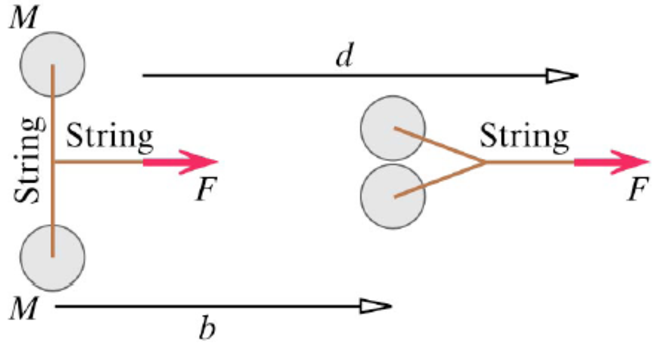
\includegraphics[width=0.6\textwidth]{figs/sliding_dumbells}

\item Santa Claus is skating on the magic ice near the North Pole, which is frictionless. A massless rope sticks out from the pole horizontally along a straight line. The rope's original length is $L_0$. Santa approaches the rope moving perpendicular to the direction of the rope and grabs the end of the rope. The diameter of the North Pole is $2a$. The rope then winds around the thin pole, $a<<L_0$, until Santa is half the original distance, $L_0/2$, from the pole. If Santa's original speed was $v_0$, what is his new speed? Assume there is no energy wasted in curving the rope around the pole. 

\item \label{Wcmproof}Prove that the work on the center of mass of a system of particles during a small time interval $\delta t$, which is defined by 
\[
\delta W_{\rm cm}\equiv \vec{F}_{\rm tot}\cdot \delta\vec{r}_{\rm cm},
\]
is equal to the change of the kinetic energy of the center of mass,
\[
T_{\rm cm}\equiv \frac{1}{2}M_{\rm tot}v_{\rm cm}^2, ~~~~~\delta T_{\rm cm}=M_{\rm tot}\vec{v}_{\rm cm}\cdot\delta\vec{v}_{\rm cm}.
\]
Use the following definitions:
\begin{eqnarray*}
\vec{F}_{\rm tot}&=&\sum_i \vec{F}_i,\\
M_{\rm tot}&=&\sum_i m_i,\\
\vec{r}_{cm}&=&\frac{1}{M_{\rm tot}}\sum_i m_i\vec{r}_i,\\
\vec{v}_{cm}&=&\frac{1}{M_{\rm tot}}\sum_i m_i\vec{v}_i.
\end{eqnarray*}

\end{enumerate} 


\newpage

\setcounter{examplecounter}{0}
% !TEX root = lectures.tex
\section{Oscillations}
\bigskip

\subsection{Harmonic Oscillator}

The harmonic oscillator is omnipresent in physics. Although students think of this as being related to springs, it, or an equivalent mathematical representation, appears in just about any problem where a mode is sitting near its potential energy minimum. At that point, $\partial_x V(x)=0$, and the first non-zero term (aside from a constant) in the potential energy is that of a harmonic oscillator. In a solid, sound modes (phonons) are built on a picture of coupled harmonic oscillators, and in relativistic field theory the fundamental interactions are also built on coupled oscillators positioned infinitesimally close to one another in space. The phenomena of a resonance of an oscillator driven at a fixed frequency plays out repeatedly in atomic, nuclear and high-energy physics, when quantum mechanically the evolution of a state oscillates according to $e^{-iEt}$ and exciting discrete quantum states has very similar mathematics as exciting discrete states of an oscillator.

The potential energy for a single particle as a function of its position $x$ can be written as a Taylor expansion about some point $x_0$
\begin{equation}
V(x)=V(x_0)+(x-x_0)\left.\partial_xV(x)\right|_{x_0}+\frac{1}{2}(x-x_0)^2\left.\partial_x^2V(x)\right|_{x_0}
+\frac{1}{3!}\left.\partial_x^3V(x)\right|_{x_0}+\cdots
\end{equation}
If the position $x_0$ is at the minimum of the resonance, the first two non-zero terms of the potential are
\begin{eqnarray}
V(x)&\approx& V(x_0)+\frac{1}{2}(x-x_0)^2\left.\partial_x^2V(x)\right|_{x_0},\\
\nonumber
&=&V(x_0)+\frac{1}{2}k(x-x_0)^2,~~~~k\equiv \left.\partial_x^2V(x)\right|_{x_0},\\
\nonumber
F&=&-\partial_xV(x)=-k(x-x_0).
\end{eqnarray}

Put into Newton's 2nd law (assuming $x_0=0$),
\begin{eqnarray}
m\ddot{x}&=&-kx,\\
x&=&A\cos(\omega_0 t-\phi),~~~\omega_0=\sqrt{k/m}.
\end{eqnarray}
Here $A$ and $\phi$ are arbitrary. Equivalently, one could have written this as $A\cos(\omega_0 t)+B\sin(\omega_0 t)$, or as the real part of $Ae^{i\omega_0 t}$. In this last case $A$ could be an arbitrary complex constant. Thus, there are 2 arbitrary constants (either $A$ and $B$ or $A$ and $\phi$, or the real and imaginary part of one complex constant. This is the expectation for a second order differential equation, and also agrees with the physical expectation that if you know a particle's initial velocity and position you should be able to define its future motion, and that those two arbitrary conditions should translate to two arbitrary constants.

A key feature of harmonic motion is that the system repeats itself after a time $T=1/f$, where $f$ is the frequency, and $\omega=2\pi f$ is the angular frequency. The period of the motion is independent of the amplitude. However, this independence is only exact when one can neglect higher terms of the potential, $x^3, x^4\cdots$. Once can neglect these terms for sufficiently small amplitudes, and for larger amplitudes the motion is no longer purely sinusoidal, and even though the motion repeats itself, the time for repeating the motion is no longer independent of the amplitude.

One can also calculate the velocity and the kinetic energy as a function of time,
\begin{eqnarray}
\dot{x}&=&-\omega_0A\sin(\omega_0 t-\phi),\\
\nonumber
T&=&\frac{1}{2}m\dot{x}^2=\frac{m\omega_0^2A^2}{2}\sin^2(\omega_0t-\phi),\\
\nonumber
&=&\frac{k}{2}A^2\sin^2(\omega_0t-\phi).
\end{eqnarray}
The total energy is then
\begin{equation}
E=T+U=\frac{1}{2}m\dot{x}^2+\frac{1}{2}kx^2=\frac{1}{2}kA^2.
\end{equation}
The total energy then goes as the square of the amplitude.

\example
A pendulum is an example of a harmonic oscillator. By expanding the kinetic and potential energies for small angles find the frequency for a pendulum of length $L$ with all the mass $m$ centered at the end by writing the eq.s of motion in the form of a harmonic oscillator.

{\bf Solution:} The potential energy and kinetic energies are (for $x$ being the displacement)
\begin{eqnarray*}
U&=&mgL(1-\cos\theta)\approx mgL\frac{x^2}{2L^2},\\
T&=&\frac{1}{2}mL^2\dot{\theta}^2\approx \frac{m}{2}\dot{x}^2.
\end{eqnarray*}
For small $x$ Newton's 2nd law becomes
\[
m\ddot{x}=-\frac{mg}{L}x,
\]
and the spring constant would appear to be $k=mg/L$, which makes the frequency equal to $\omega_0=\sqrt{g/L}$. Note that the frequency is independent of the mass.

\exampleend

\subsection{Damped Oscillators}

In this chapter we consider only the case where the damping force is proportional to the velocity. This is counter to dragging friction, where the force is proportional in strength to the normal force and independent of velocity, and is also inconsistent with wind resistance, where the magnitude of the drag force is proportional the square of the velocity. Rolling resistance does seem to be mainly proportional to the velocity. However, the main motivation for considering damping forces proportional to the velocity is that the math is more friendly. This is because the differential equation is linear, i.e. each term is of order $x$, $\dot{x}$, $\ddot{x}\cdots$, or even terms with no mention of $x$, and there are no terms such as $x^2$ or $x\ddot{x}$. The equations of motion for a spring with damping force $-b\dot{x}$ are
\begin{equation}
m\ddot{x}+b\dot{x}+kx=0.
\end{equation}
Just to make the solution a bit less messy, we rewrite this equation as
\begin{equation}
\label{eq:dampeddiffyq}
\ddot{x}+2\beta\dot{x}+\omega_0^2x=0,~~~~\beta\equiv b/2m,~\omega_0\equiv\sqrt{k/m}.
\end{equation}
Both $\beta$ and $\omega$ have dimensions of inverse time. To find solutions (see appendix C in the text) you must make an educated guess at the form of the solution. To do this, first realize that the solution will need an arbitrary normalization $A$ because the equation is linear. Secondly, realize that if the form is
\begin{equation}
x=Ae^{rt}
\end{equation}
that each derivative simply brings out an extra power of $r$. This means that the $Ae^{rt}$ factors out and one can simply solve for an equation for $r$. Plugging this form into Eq. (\ref{eq:dampeddiffyq}),
\begin{equation}
r^2+2\beta r+\omega_0^2=0.
\end{equation}
Because this is a quadratic equation there will be two solutions,
\begin{equation}
r=-\beta\pm\sqrt{\beta^2-\omega_0^2}.
\end{equation}
We refer to the two solutions as $r_1$ and $r_2$ corresponding to the $+$ and $-$ roots. As expected, there should be two arbitrary constants involved in the solution,
\begin{equation}
x=A_1e^{r_1t}+A_2e^{r_2t},
\end{equation}
where the coefficients $A_1$ and $A_2$ are determined by initial conditions.

The roots listed above, $\sqrt{\omega_0^2-\beta_0^2}$, will be imaginary if the damping  is small and $\beta<\omega_0$. In that case, $r$ is complex and the factor $e{rt}$ will have some oscillatory behavior. If the roots are real, there will only be exponentially decaying solutions. There are three cases:
\begin{enumerate}\itemsep 0pt
\item Underdamped: $\beta<\omega_0$
\begin{eqnarray}
x&=&A_1e^{-\beta t}e^{i\omega't}+A_2e^{-\beta t}e^{-i\omega't},~~\omega'\equiv\sqrt{\omega_0^2-\beta^2}\\
\nonumber
&=&(A_1+A_2)e^{-\beta t}\cos\omega't+i(A_1-A_2)e^{-\beta t}\sin\omega't.
\end{eqnarray}
Here we have made use of the identity $e^{i\omega't}=\cos\omega't+i\sin\omega't$. Because the constants are arbitrary, and because the real and imaginary parts are both solutions individually, we can simply consider the real part of the solution alone:
\begin{eqnarray}
\label{eq:homogsolution}
x&=&B_1e^{-\beta t}\cos\omega't+B_2e^{-\beta t}\sin\omega't,\\
\nonumber 
\omega'&\equiv&\sqrt{\omega_0^2-\beta^2}.
\end{eqnarray}

\item Critical dampling: $\beta=\omega_0$\\
In this case the two terms involving $r_1$ and $r_2$ are identical because $\omega'=0$. Because we need to arbitrary constants, there needs to be another solution. This is found by simply guessing, or by taking the limit of $\omega'\rightarrow 0$ from the underdamped solution. The solution is then
\begin{equation}
\label{eq:criticallydamped}
x=Ae^{-\beta t}+Bte^{-\beta t}.
\end{equation}
The critically damped solution is interesting because the solution approaches zero quickly, but does not oscillate. For a problem with zero initial velocity, the solution never crosses zero. This is a good choice for designing shock absorbers or swinging doors.
\item Overdamped: $\beta>\omega_0$
\begin{eqnarray}
x&=&A_1e^{-(\beta+\sqrt{\beta^2-\omega_0^2})t}+A_2e^{-(\beta-\sqrt{\beta^2-\omega_0^2})t}
\end{eqnarray}
This solution will also never pass the origin more than once, and then only if the initial velocity is strong and initially toward zero.
\end{enumerate}

\example
Given $b$, $m$ and $\omega_0$, find $x(t)$ for a particle whose initial position is $x=0$ and has initial velocity $v_0$ (assuming an underdamped solution).

{\bf Solution:} The solution is of the form,
\begin{eqnarray*}
x&=&e^{-\beta t}\left[A_1\cos(\omega' t)+A_2\sin\omega't\right],\\
\dot{x}&=&-\beta x+\omega'e^{-\beta t}\left[-A_1\sin\omega't+A_2\cos\omega't\right].\\
\omega'&\equiv&\sqrt{\omega_0^2-\beta^2},~~~\beta\equiv b/2m.
\end{eqnarray*}
From the initial conditions, $A_1=0$ because $x(0)=0$ and $\omega'A_2=v_0$. So 
\[
x=\frac{v_0}{\omega'}e^{-\beta t}\sin\omega't.
\]
\exampleend

\subsection{Sinusoidally Driven Oscillators}

Here, we consider the force
\begin{equation}
F=-kx-b\dot{x}+F_0\cos\omega t,
\end{equation}
which leads to the differential equation
\begin{equation}
\label{eq:drivenosc}
\ddot{x}+2\beta\dot{x}+\omega_0^2x=(F_0/m)\cos\omega t.
\end{equation}
Consider a single solution with no arbitrary constants, which we will call a {\it particular solution}, $x_p(t)$. It should be emphasized that this is {\bf A} particular solution, because there exists an infinite number of such solutions because the general solution should have two arbitrary constants. Now consider solutions to the same equation without the driving term, which include two arbitrary constants. These are called either {\it homogenous solutions} or {\it complementary solutions}, and were given in the previous section, e.g. Eq. (\ref{eq:homogsolution}) for the underdamped case. The homogenous solution already incorporates the two arbitrary constants, so any sum of a homogenous solution and a particular solution will represent the {\it general solution} of the equation. The general solution incorporates the two arbitrary constants $A$ and $B$ to accommodate the two initial conditions. One could have picked a different particular solution, i.e. the original particular solution plus any homogenous solution with the arbitrary constants $A_p$ and $B_p$ chosen at will. When one adds in the homogenous solution, which has adjustable constants with arbitrary constants $A'$ and $B'$, to the new particular solution, one can get the same general solution by simply adjusting the new constants such that $A'+A_p=A$ and $B'+B_p=B$. Thus, the choice of $A_p$ and $B_p$ are irrelevant, and when choosing the particular solution it is best to make the simplest choice possible.

To find a particular solution, one first guesses at the form,
\begin{equation}
\label{eq:partform}
x_p(t)=D\cos(\omega t-\delta),
\end{equation}
and rewrite the differential equation as
\begin{equation}
D\left\{-\omega^2\cos(\omega t-\delta)-2\beta\omega\sin(\omega t-\delta)+\omega_0^2\cos(\omega t-\delta)\right\}=\frac{F_0}{m}\cos(\omega t).
\end{equation}
One can now use angle addition formulas to get
\begin{eqnarray}
D\left\{(-\omega^2\cos\delta+2\beta\omega\sin\delta+\omega_0^2\cos\delta)\cos(\omega t)\right.\hspace*{36pt}&&\\
\nonumber
\left.+(-\omega^2\sin\delta-2\beta\omega\cos\delta+\omega_0^2\sin\delta)\sin(\omega t)\right\}
&=&\frac{F_0}{m}\cos(\omega t).
\end{eqnarray}
Both the $\cos$ and $\sin$ terms need to equate if the expression is to hold at all times. Thus, this becomes two equations
\begin{eqnarray}
D\left\{-\omega^2\cos\delta+2\beta\omega\sin\delta+\omega_0^2\cos\delta\right\}&=&\frac{F_0}{m}\\
\nonumber
-\omega^2\sin\delta-2\beta\omega\cos\delta+\omega_0^2\sin\delta&=&0.
\end{eqnarray}
After dividing by $\cos\delta$, the lower expression leads to
\begin{equation}
\tan\delta=\frac{2\beta\omega}{\omega_0^2-\omega^2}.
\end{equation}
Using the identities $\tan^2+1=\csc^2$ and $\sin^2+\cos\^2=1$, one can also express $\sin\delta$ and $\cos\delta$,
\begin{eqnarray}
\sin\delta&=&\frac{2\beta\omega}{\sqrt{(\omega_0^2-\omega^2)^2+4\omega^2\beta^2}},\\
\nonumber
\cos\delta&=&\frac{(\omega_0^2-\omega^2)}{\sqrt{(\omega_0^2-\omega^2)^2+4\omega^2\beta^2}}
\end{eqnarray}
Inserting the expressions for $\cos\delta$ and $\sin\delta$ into the expression for $D$,
\begin{equation}
\label{eq:Ddrive}
D=\frac{F_0/m}{\sqrt{(\omega_0^2-\omega^2)^2+4\omega^2\beta^2}}.
\end{equation}

For a given initial condition, e.g. initial displacement and velocity, one must add the homogenous solution then solve for the two arbitrary constants. However, because the homogenous solutions decay with time as $e^{-\beta t}$, the particular solution is all that remains at large times, and is therefore the steady state solution. Because the arbitrary constants are all in the homogenous solution, all memory of the initial conditions are lost at large times, $t>>1/\beta$.

The amplitude of the motion, $D$, is linearly proportional to the driving force ($F_0/m$), but also depends on the driving frequency $\omega$. For small $\beta$ the maximum will occur at $\omega=\omega_0$. This is referred to as a resonance. In the limit $\beta\rightarrow 0$ the amplitude at resonance approaches infinity. 

\subsection{Alternative Derivation for Driven Oscillators}

Here, we derive the same expressions as in Eq.s (\ref{eq:partform}-\ref{eq:Ddrive}) but express the driving forces as
\begin{eqnarray}
F(t)&=&F_0e^{i\omega t},
\end{eqnarray}
rather than as $F_0\cos\omega t$. The real part of $F$ is the same as before. For the differential equation,
\begin{eqnarray}
\label{eq:compdrive}
\ddot{x}+2\beta\dot{x}+\omega_0^2x&=&\frac{F_0}{m}e^{i\omega t},
\end{eqnarray}
one can treat $x(t)$ as an imaginary function. Because the operations $d^2/dt^2$ and $d/dt$ are real and thus do not mix the real and imaginary parts of $x(t)$, Eq. (\ref{eq:compdrive}) is effectively 2 equations. Because $e^{\omega t}=\cos\omega t+i\sin\omega t$, the real part of the solution for $x(t)$ gives the solution for a driving force $F_0\cos\omega t$, and the imaginary part of $x$ corresponds to the case where the driving force is $F_0\sin\omega t$. It is rather easy to solve for the complex $x$ in this case, and by taking the real part of the solution, one finds the answer for the $\cos\omega t$ driving force.

We assume a simple form for the particular solution
\begin{equation}
x_p=De^{i\omega t},
\end{equation}
where $D$ is a complex constant.

From Eq. (\ref{eq:compdrive}) one inserts the form for $x_p$ above to get
\begin{eqnarray}
D\left\{-\omega^2+2i\beta\omega+\omega_0^2\right\}e^{i\omega t}=(F_0/m)e^{i\omega t},\\
\nonumber
D=\frac{F_0/m}{(\omega_0^2-\omega^2)+2i\beta\omega}.
\end{eqnarray}
The norm and phase for $D=|D|e^{-i\delta}$ can be read by inspection,
\begin{equation}
|D|=\frac{F_0/m}{\sqrt{(\omega_0^2-\omega^2)^2+4\beta^2\omega^2}},~~~~\tan\delta=\frac{2\beta\omega}{\omega_0^2-\omega^2}.
\end{equation}
This is the same expression for $\delta$ as before. One then finds $x_p(t)$,
\begin{eqnarray}
\label{eq:fastdriven1}
x_p(t)&=&\Re\frac{(F_0/m)e^{i\omega t-i\delta}}{\sqrt{(\omega_0^2-\omega^2)^2+4\beta^2\omega^2}}\\
\nonumber
&=&\frac{(F_0/m)\cos(\omega t-\delta)}{\sqrt{(\omega_0^2-\omega^2)^2+4\beta^2\omega^2}}.
\end{eqnarray}
This is the same answer as before.
If one wished to solve for the case where $F(t)= F_0\sin\omega t$, the imaginary part of the solution would work
\begin{eqnarray}
\label{eq:fastdriven2}
x_p(t)&=&\Im\frac{(F_0/m)e^{i\omega t-i\delta}}{\sqrt{(\omega_0^2-\omega^2)^2+4\beta^2\omega^2}}\\
\nonumber
&=&\frac{(F_0/m)\sin(\omega t-\delta)}{\sqrt{(\omega_0^2-\omega^2)^2+4\beta^2\omega^2}}.
\end{eqnarray}

\example
Consider the damped and driven harmonic oscillator worked out above. Given $F_0, m,\beta$ and $\omega_0$, solve for the complete solution $x(t)$ for the case where $F=F_0\sin\omega t$ with initial conditions $x(t=0)=0$ and $v(t=0)=0$. Assume the underdamped case.

{\bf Solution:}
The general solution including the arbitrary constants includes both the homogenous and particular solutions,
\begin{eqnarray*}
x(t)&=&\frac{F_0}{m}\frac{\sin(\omega t-\delta)}{\sqrt{(\omega_0^2-\omega^2)^2+4\beta^2\omega^2}}
+A\cos\omega't e^{-\beta t}+B\sin\omega't e^{-\beta t}.
\end{eqnarray*}
The quantities $\delta$ and $\omega'$ are given earlier in the section, $\omega'=\sqrt{\omega_0^2-\beta^2}, \delta=\tan^{-1}(2\beta\omega/(\omega_0^2-\omega^2)$. Here, solving the problem means finding the arbitrary constants $A$ and $B$. Satisfying the initial conditions for the initial position and velocity:
\begin{eqnarray*}
x(t=0)=0&=&-\eta\sin\delta+A,\\
v(t=0)=0&=&\omega\eta\cos\delta-\beta A+\omega'B,\\
\eta&\equiv&\frac{F_0}{m}\frac{1}{\sqrt{(\omega_0^2-\omega^2)^2+4\beta^2\omega^2}}.
\end{eqnarray*}
The problem is now reduced to 2 equations and 2 unknowns, $A$ and $B$. The solution is
\begin{eqnarray}
A&=& \eta\sin\delta ,~~~B=\frac{-\omega\eta\cos\delta+\beta\eta\sin\delta}{\omega'}.
\end{eqnarray}

\exampleend

\subsection{Resonance Widths; the $Q$ factor}

From the previous two sections, the particular solution for a driving force, $F=F_0\cos\omega t$, is
\begin{eqnarray}
x_p(t)&=&\frac{F_0/m}{\sqrt{(\omega_0^2-\omega^2)^2+4\omega^2\beta^2}}\cos(\omega_t-\delta),\\
\nonumber
\delta&=&\tan^{-1}\left(\frac{2\beta\omega}{\omega_0^2-\omega^2}\right).
\end{eqnarray}
If one fixes the driving frequency $\omega$ and adjusts the fundamental frequency $\omega_0=\sqrt{k/m}$, the maximum amplitude occurs when $\omega_0=\omega$ because that is when the term from the denominator $(\omega_0^2-\omega^2)^2+4\omega^2\beta^2$ is at a minimum. This is akin to dialing into a radio station. However, if one fixes $\omega_0$ and adjusts the driving frequency one minimize with respect to $\omega$, e.g. set 
\begin{equation}
\frac{d}{d\omega}\left[(\omega_0^2-\omega^2)^2+4\omega^2\beta^2\right]=0,
\end{equation}
and one finds that the maximum amplitude occurs when $\omega=\sqrt{\omega_0^2-2\beta^2}$. If $\beta$ is small relative to $\omega_0$, one can simply state that the maximum amplitude is
\begin{equation}
x_{\rm max}\approx\frac{F_0}{2m\beta \omega_0}.
\end{equation}
\begin{figure}
\centerline{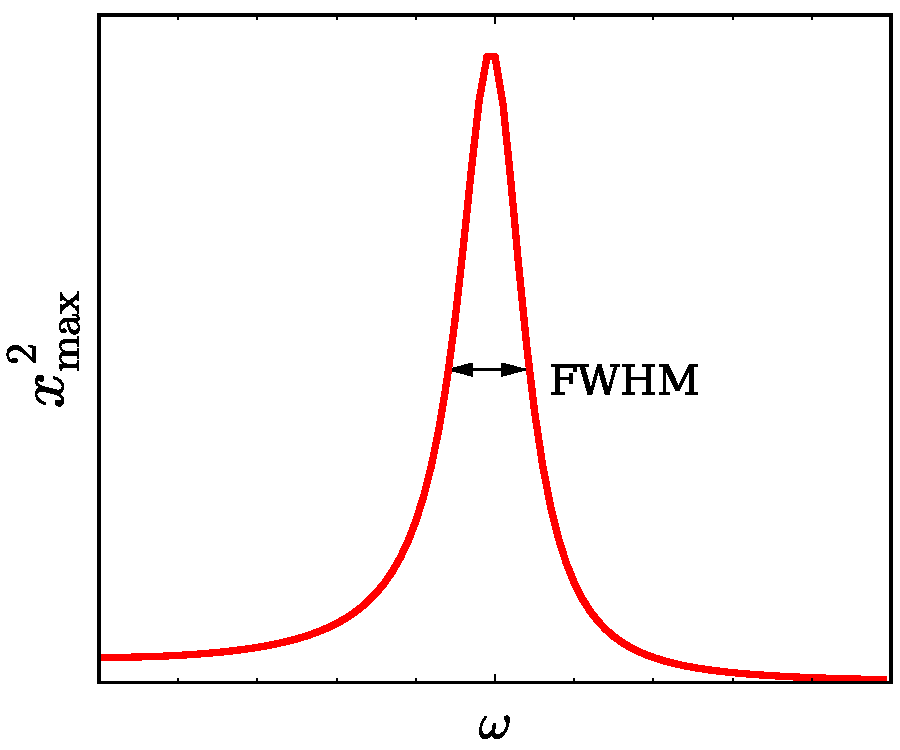
\includegraphics[width=0.32\textwidth]{figs/qfactor}}
\caption{\label{fig:qfactor}
The maximum amplitude squared of the steady-state motion of a sinusoidally driven harmonic oscillator is shown as a function of the driving frequency $\omega$. This peaks near the fundamental frequency $\omega_0$ and the full-width-half-maximum, $FWHM$, is given by the damping, $2\beta$.}
\end{figure}
Figure \ref{fig:qfactor} displays the maximum amplitude squared as a function of $\omega$, and  one can see the peak at $\omega\approx\omega_0$. The squared amplitude is usually more the quantity of interest than the amplitude because the power being absorbed by the oscillator is proportional to the square of the amplitude, not the amplitude. The width of the peak is quantified by the full-width-half-maximum, sometimes called $FWHM$ and can be found by finding the frequency difference, $\omega-\omega_0$, such that the maximum response falls by a factor of two,
\begin{eqnarray}
\frac{4\omega^2\beta^2}{(\omega_0^2-\omega^2)^2+4\omega^2\beta^2}=\frac{1}{2}.
\end{eqnarray}
For small damping this occurs when $\omega=\omega_0\pm \beta$, so the $FWHM\approx 2\beta$. For the purposes of tuning to a specific frequency, one wants the width to be as small as possible. The ratio of $\omega_0$ to $FWHM$ is known as the {\it quality} factor, or $Q$ factor,
\begin{equation}
Q\equiv \frac{\omega_0}{2\beta}.
\end{equation}

\subsection{Principal of Superposition and Periodic Forces (Fourier Transforms)}

If one has several driving forces, $F(t)=\sum_n F_n(t)$, one can find the particular solution to each $F_n$, $x_{pn}(t)$, and the particular solution for the entire driving force is 
\begin{equation}
x_p(t)=\sum_nx_{pn}(t).
\end{equation}
This is known as the principal of superposition. It only applies when the homogenous equation is linear. If there were an anharmonic term such as $x^3$ in the homogenous equation, then when one summed various solutions, $x=(\sum_n x_n)^2$, one would get cross terms. Superposition is especially useful when $F(t)$ can be written as a sum of sinusoidal terms, because the solutions for each sinusoidal term is analytic, and are given in the previous two subsections. 

Driving forces are often periodic, even when they are not sinusoidal. Periodicity implies that for some time $\tau$
\begin{eqnarray}
F(t+\tau)=F(t). 
\end{eqnarray}
One example of a non-sinusoidal periodic force is a square wave. Many components in electric circuits are non-linear, e.g. diodes, which makes many wave forms non-sinusoidal even when the circuits are being driven by purely sinusoidal sources.

For the sinusoidal example studied in the previous subsections the period is $\tau=2\pi/\omega$. However, higher harmonics can also satisfy the periodicity requirement. In general, any force that satisfies the periodicity requirement can be expressed as a sum over harmonics,
\begin{equation}
F(t)=\frac{f_0}{2}+\sum_{n>0} f_n\cos(2n\pi t/\tau)+g_n\sin(2n\pi t/\tau).
\end{equation}
From the previous subsection, one can write down the answer for $x_{pn}(t)$, by substituting $f_n/m$ or $g_n/m$ for $F_0/m$ into Eq.s (\ref{eq:fastdriven1}) or (\ref{eq:fastdriven2}) respectively. By writing each factor $2n\pi t/\tau$ as $n\omega t$, with $\omega\equiv 2\pi/\tau$,
\begin{equation}
\label{eq:fourierdef1}
F(t)=\frac{f_0}{2}+\sum_{n>0}f_n\cos(n\omega t)+g_n\sin(n\omega t).
\end{equation}
The solutions for $x(t)$ then come from replacing $\omega$ with $n\omega$ for each term in the particular solution in Eq.s (\ref{eq:partform}-\ref{eq:Ddrive}),
\begin{eqnarray}
x_p(t)&=&\frac{f_0}{2k}+\sum_{n>0} \alpha_n\cos(n\omega t-\delta_n)+\beta_n\sin(n\omega t-\delta_n),\\
\nonumber
\alpha_n&=&\frac{f_n/m}{\sqrt{((n\omega)^2-\omega_0^2)+4\beta^2n^2\omega^2}},\\
\nonumber
\beta_n&=&\frac{g_n/m}{\sqrt{((n\omega)^2-\omega_0^2)+4\beta^2n^2\omega^2}},\\
\nonumber
\delta_n&=&\tan^{-1}\left(\frac{2\beta n\omega}{\omega_0^2-n^2\omega^2}\right).
\end{eqnarray}
Because the forces have been applied for a long time, any non-zero damping eliminates the homogenous parts of the solution, so one need only consider the particular solution for each $n$.

The problem will considered solved if one can find expressions for the coefficients $f_n$ and $g_n$, even though the solutions are expressed as an infinite sum. The coefficients can be extracted from the function $F(t)$ by
\begin{eqnarray}
\label{eq:fourierdef2}
f_n&=&\frac{2}{\tau}\int_{-\tau/2}^{\tau/2} dt~F(t)\cos(2n\pi t/\tau),\\
\nonumber
g_n&=&\frac{2}{\tau}\int_{-\tau/2}^{\tau/2} dt~F(t)\sin(2n\pi t/\tau).
\end{eqnarray}

To check the consistency of these expressions and to verify Eq. (\ref{eq:fourierdef2}), one can insert the expansion of $F(t)$ in Eq. (\ref{eq:fourierdef1}) into the expression for the coefficients in Eq. (\ref{eq:fourierdef2}) and see whether
\begin{eqnarray}
f_n&=?&\frac{2}{\tau}\int_{-\tau/2}^{\tau/2} dt~\left\{
\frac{f_0}{2}+\sum_{m>0}f_m\cos(m\omega t)+g_m\sin(m\omega t)
\right\}\cos(n\omega t).
\end{eqnarray}
Immediately, one can throw away all the terms with $g_m$ because they convolute an even and an odd function. The term with $f_0/2$ disappears because $\cos(n\omega t)$ is equally positive and negative over the interval and will integrate to zero. For all the terms $f_m\cos(m\omega t)$ appearing in the sum, one can use angle addition formulas to see that $\cos(m\omega t)\cos(n\omega t)=(1/2)(\cos[(m+n)\omega t]+\cos[(m-n)\omega t]$. This will integrate to zero unless $m=n$. In that case the $m=n$ term gives
\begin{equation}
\int_{-\tau/2}^{\tau/2}dt~\cos^2(m\omega t)=\frac{\tau}{2},
\end{equation}
and
\begin{eqnarray}
f_n&=?&\frac{2}{\tau}\int_{-\tau/2}^{\tau/2} dt~f_n/2\\
\nonumber
&=&f_n~\checkmark.
\end{eqnarray}
The same method can be used to check for the consistency of $g_n$.

\example
Consider the driving force:
\begin{equation}
F(t)=At/\tau,~~-\tau/2<t<\tau/2,~~~F(t+\tau)=F(t).
\end{equation}
Find the Fourier coefficients $f_n$ and $g_n$ for all $n$ using Eq. (\ref{eq:fourierdef2}).

{\bf Solution:} Only the odd coefficients enter by symmetry, i.e. $f_n=0$. One can find $g_n$ integrating by parts,
\begin{eqnarray}
\label{eq:fouriersolution}
g_n&=&\frac{2}{\tau}\int_{-\tau/2}^{\tau/2}dt~\sin(n\omega t) \frac{At}{\tau}\\
\nonumber
u&=&t,~dv=\sin(n\omega t)dt,~v=-\cos(n\omega t)/(n\omega),\\
\nonumber
g_n&=&\frac{-2A}{n\omega \tau^2}\int_{-\tau/2}^{\tau/2}dt~\cos(n\omega t)
+\left.2A\frac{-t\cos(n\omega t)}{n\omega\tau^2}\right|_{-\tau/2}^{\tau/2}.
\end{eqnarray}
The first term is zero because $\cos(n\omega t)$ will be equally positive and negative over the interval. Using the fact that $\omega\tau=2\pi$,
\begin{eqnarray}
g_n&=&-\frac{2A}{2n\pi}\cos(n\omega\tau/2)\\
\nonumber
&=&-\frac{A}{n\pi}\cos(n\pi)\\
\nonumber
&=&\frac{A}{n\pi}(-1)^{n+1}.
\end{eqnarray}
The true function is compared to the expansion in Fig. \ref{fig:triangle} where the sum is cut off at finite $n$.
\begin{figure}
\centerline{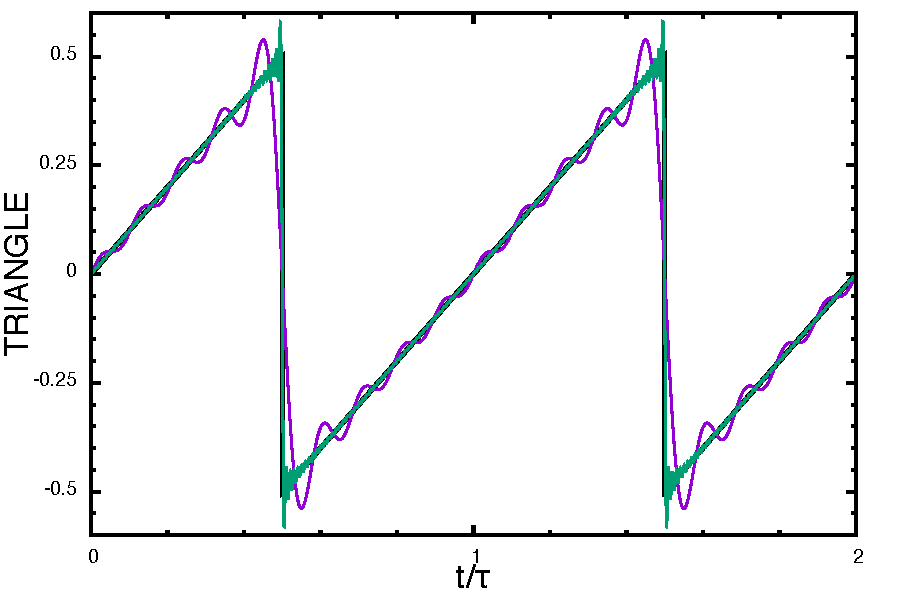
\includegraphics[width=0.6\textwidth]{figs/triangle}}
\caption{\label{fig:triangle}
The periodic function $F(t)=t/\tau, |t|<\tau/2$ (black) is compared to the Fourier expansion described in Eq. (\ref{eq:fouriersolution}) with 10 terms (red) or 100 terms (green).}
\end{figure}

\exampleend

\subsection{Response to Transient Force}

Consider a particle at rest in the bottom of an underdamped harmonic oscillator, that then feels a sudden impulse, or change in momentum, $I=F\Delta t$ at $t=0$. This increases the velocity immediately by an amount $v_0=I/m$ while not changing the position. One can then solve the trajectory by solving Eq. (\ref{eq:homogsolution}) with initial conditions $v_0=I/m$ and $x_0=0$. This gives
\begin{equation}
x(t)=\frac{I}{m\omega'}e^{-\beta t}\sin\omega't, ~~t>0.
\end{equation}
Here, $\omega'=\sqrt{\omega_0^2-\beta^2}$. For an impulse $I_i$ that occurs at time $t_i$ the trajectory would be
\begin{equation}
x(t)=\frac{I_i}{m\omega'}e^{-\beta (t-t_i)}\sin[\omega'(t-t_i)] \Theta(t-t_i),
\end{equation}
where $\Theta(t-t_i)$ is a step function, i.e. $\Theta(x)$ is zero for $x<0$ and unity for $x>0$. If there were several impulses linear superposition tells us that we can sum over each contribution,
\begin{equation}
x(t)=\sum_i\frac{I_i}{m\omega'}e^{-\beta(t-t_i)}\sin[\omega'(t-t_i)]\Theta(t-t_i)
\end{equation} 

Now one can consider a series of impulses at times separated by $\Delta t$, where each impulse is given by $F_i\Delta t$. The sum above now becomes an integral,
\begin{eqnarray}\label{eq:Greeny}
x(t)&=&\int_{-\infty}^\infty dt'~F(t')\frac{e^{-\beta(t-t')}\sin[\omega'(t-t')]}{m\omega'}\Theta(t-t')\\
\nonumber
&=&\int_{-\infty}^\infty dt'~F(t')G(t-t'),\\
\nonumber
G(\Delta t)&=&\frac{e^{-\beta\Delta t}\sin[\omega' \Delta t]}{m\omega'}\Theta(\Delta t)
\end{eqnarray}
The quantity $e^{-\beta(t-t')}\sin[\omega'(t-t')]/m\omega'\Theta(t-t')$ is called a Green's function, $G(t-t')$. It describes the response at $t$ due to a force applied at a time $t'$, and is a function of $t-t'$. The step function ensures that the response does not occur before the force is applied. One should remember that the form for $G$ would change if the oscillator were either critically- or over-damped.

When performing the integral in Eq. (\ref{eq:Greeny}) one can use angle addition formulas to factor out the part with the $t'$ dependence in the integrand,
\begin{eqnarray}
\label{eq:Greeny2}
x(t)&=&\frac{1}{m\omega'}e^{-\beta t}\left[I_c(t)\sin(\omega't)-I_s(t)\cos(\omega't)\right],\\
\nonumber
I_c(t)&\equiv&\int_{-\infty}^t dt'~F(t')e^{\beta t'}\cos(\omega't'),\\
\nonumber
I_s(t)&\equiv&\int_{-\infty}^t dt'~F(t')e^{\beta t'}\sin(\omega't').
\end{eqnarray}
If the time $t$ is beyond any time at which the force acts, $F(t'>t)=0$, the coefficients $I_c$ and $I_s$ become independent of $t$. 

\example
Consider an undamped oscillator ($\beta\rightarrow 0$), with characteristic frequency $\omega_0$ and mass $m$, that is at rest until it feels a force described by a Gaussian form,
\begin{eqnarray*}
F(t)&=&F_0 \exp\left\{\frac{-t^2}{2\tau^2}\right\}.
\end{eqnarray*}
For large times ($t>>\tau$), where the force has died off, find $x(t)$.\\
{\bf Solution:} Solve for the coefficients $I_c$ and $I_s$ in Eq. (\ref{eq:Greeny2}). Because the Gaussian is an even function, $I_s=0$, and one need only solve for $I_c$,
\begin{eqnarray*}
I_c&=&F_0\int_{-\infty}^\infty dt'~e^{-t^{\prime 2}/(2\tau^2)}\cos(\omega_0 t')\\
&=&\Re F_0 \int_{-\infty}^\infty dt'~e^{-t^{\prime 2}/(2\tau^2)}e^{i\omega_0 t'}\\
&=&\Re F_0 \int_{-\infty}^\infty dt'~e^{-(t'-i\omega_0\tau^2)^2/(2\tau^2)}e^{-\omega_0^2\tau^2/2}\\
&=&F_0\tau \sqrt{2\pi} e^{-\omega_0^2\tau^2/2}.
\end{eqnarray*}
The third step involved completing the square, and the final step used the fact that the integral
\begin{eqnarray*}
\int_{-\infty}^\infty dx~e^{-x^2/2}&=&\sqrt{2\pi}.
\end{eqnarray*}
To see that this integral is true, consider the square of the integral, which you can change to polar coordinates,
\begin{eqnarray*}
I&=&\int_{-\infty}^\infty dx~e^{-x^2/2}\\
I^2&=&\int_{-\infty}^\infty dxdy~e^{-(x^2+y^2)/2}\\
&=&2\pi\int_0^\infty rdr~e^{-r^2/2}\\
&=&2\pi.
\end{eqnarray*}
Finally, the expression for $x$ from Eq. (\ref{eq:Greeny2}) is
\begin{eqnarray*}
x(t>>\tau)&=&\frac{F_0\tau}{m\omega_0} \sqrt{2\pi} e^{-\omega_0^2\tau^2/2}\sin(\omega_0t).
\end{eqnarray*}


\exampleend

\subsection{Solving Equations of Motion Numerically}
%If one has a known force $F(t)$, and initial conditions $x(t=0)=x_0$ and $v(t=0)=v_0$, one can solve for the equations of motion numerically. First, one must choose a small time step $\Delta t$, smaller than any characteristic time scale of the problem. One can then define a mesh $x_n$, where $n=0$ so some maximum number of steps $N$. We will defines these values as
\begin{eqnarray}
x_n=x(n\Delta t).
\end{eqnarray}
Assume that one knows $x_n$ for all $i<\le j$. One can express the velocities and accelerations in Newton's equations of motion for a mass $m$ as:

\begin{eqnarray}
v_n&=&\frac{x_{n+1}-x_{n-1}}{2\Delta t},\\
\nonumber
a_n&=&\frac{v_{n+1/2}-v_{n-1/2}}{\Delta t}\\
\nonumber
&=&\frac{x_{n+1}-2x_n+x_{n-1}}{(\Delta t)^2}.
\end{eqnarray}
The equations of motion at $t_n=n\Delta t$ become
\begin{eqnarray}
F(x_n)&=&ma_n.
\end{eqnarray}
If one knows $x_{n-1}$ and $x_n$ the only unknown in the equation is $x_{n+1}$. One can solve for it, then move onto the next $n$. Note that to proceed one needs to know $x$ at two points. This can be tricky depending on how the initial conditions are specified. 

\example
Write a numerical program to solve the evolution of a particle of mass $m$ feeling a spring force, $-kx$ and a drag force, $-bv$. Assume there is also some external force, $F(t)=F_0\sin\omega t$. Let the initial conditions be $x(t=0)=0$ and $v(t=0)=v_0$.

{\bf Solution:} The differential equation,
\begin{eqnarray*}
m\ddot{x}+b\dot{x}+kx&=&0,\\
\end{eqnarray*}
becomes
\begin{eqnarray*}
\frac{m}{(\Delta t)^2}\left(x_{n+1}-2x_n+x_{n-1}\right)+\frac{b}{2\Delta t}\left(x_{n+1}-x_{n-1}\right)+kx_n&=&F(n\Delta t).
\end{eqnarray*}
Solving for $x_{n+1}$,
\begin{eqnarray*}
\left\{\frac{m}{(\Delta t)^2}+\frac{b}{2\Delta t}\right\}x_{n+1}&=&\left[\frac{2m}{(\Delta t)^2}-k\right]x_n+F(n\Delta t)
+\left[-\frac{m}{(\Delta t)^2}+\frac{b}{2\Delta t}\right]x_{n-1},\\
x_{n+1}&=&\frac{\left[\frac{2m}{(\Delta t)^2}-k\right]x_n+F(n\Delta t)
+\left[-\frac{m}{(\Delta t)^2}+\frac{b}{2\Delta t}\right]x_{n-1}}{\frac{m}{(\Delta t)^2}+\frac{b}{2\Delta t}}.
\end{eqnarray*}
In order to iterate forward to find $x_{n+1}$, one must know $x_{n-1}$ and $x_n$. However, to get started, one only knows one value of $x$, along with the velocity being zero. To get $x$ at two time steps, one must can use the above two pieces of information,
\begin{eqnarray*}
v_0&=&\frac{x_1-x_{-1}}{2\Delta t},\\
-bv_0-kx_0&=&m\frac{x_1-2x_0+x_{-1}}{\Delta t^2},
\end{eqnarray*}
then combine the equations to eliminate $x_{-1}$ to solve for $x_1$. The fact that $x_0=0$ makes the algebra simpler,
\begin{eqnarray*}
x_1&=&v_0\Delta t-\frac{bv_0\Delta t^2}{2m}.
\end{eqnarray*}



The program might read:
{\tt\begin{verbatim}
double F(double t){
   double F0=????,omega=????;
   return F0*sin(omega*t);
}
void main(){
   const int Ntsteps=???;
   double x[Ntsteps+1],dt=???,k=???,m=???,b=???,v0=???;
   x[0] = 0.0;
   x[1] = v0*dt-0.5*b*v0/m;
   for(int it=1;it<Ntsteps;it=it+1){
      x[it+1]=( (2.0*m/(dt*dt)) -k)*x[it] + F(it*dt)
      + (0.5*b/dt)*x[it-1] ) / ( (m/(dt*dt) + 0.5*b/dt );
   }
}
\end{verbatim}}
Question marks would be replaced by the given parameters of the problem.

\exampleend

\subsection{Exercises}

\begin{enumerate}

\item A floating body of uniform cross-sectional area $A$ and of mass density $\rho$ and at equilibrium displaces a volume $V$. Show that the period of small oscillations about the equilibrium position is given by 
\[
\tau=2\pi\sqrt{V/gA}
\]

\item Show that the critically damped solution, Eq. (\ref{eq:criticallydamped}), is indeed the solution to the differential equation.

\item Consider an over-damped harmonic oscillator with a mass of $m=2$ kg, a damping factor $b=20$ Ns/m, and a spring constant $k=32$ N/m. If the initial position is $x=0.125$ m, and if the initial velocity is $-2.0$ m/s, find and graph the motion as a function of time. Graphically, find the time at which the mass crosses the origin.

\item Consider a particle of mass $m$ moving in a one-dimensional potential,
\[
V(x)=-k\frac{x^2}{2}+\alpha\frac{x^4}{4}.
\]
\begin{enumerate}
\item What is the angular frequency for small vibrations about the minimum of the potential? What is the effective spring constant?
\item If you add a small force $F=F_0\cos(\omega t-\phi)$, and if the particle is initially at the minimum with zero initial velocity, find its position as a function of time.
\item If there is a small drag force $-bv$, repeat (b).
\end{enumerate}

\item Consider the periodic force, $F(t+\tau)=F(t)$,
\[
F(t)=\left\{\begin{array}{rl}
-A,&-\tau/2<t<0\\
+A,&0<t<\tau/2
\end{array}\right.
\]
Find the coefficients $f_n$ and $g_n$ defined in Eq. (\ref{eq:fourierdef2}).

\item A ``delta'' function is a function that is zero everywhere except where the argument is zero. At this point the function is infinite so that the area under the curve is unity. The delta function obeys the relations
\begin{eqnarray*}
\int_a^b dt'~ \delta(t'-t_0)&=&1,\\
\int_a^b dt'~ f(t')\delta(t'-t_0)&=&f(t_0),
\end{eqnarray*}
as long as the time $t_0$ lies between the limits $a$ and $b$. Otherwise, the integrals are zero.
\begin{enumerate}
\item Show that the following function
\[
\left.\frac{1}{\pi}\frac{\Lambda}{\Lambda^2+x^2}\right|_{\Lambda\rightarrow 0}=\delta(x).
\]
i.e. show that it is zero everywhere except the origin and that it integrates to unity.
\item A step function, $\Theta(t)$, a.k.a. the ``Theta'' function or the Heaviside function, is zero for negative arguments and is unity for positive arguments. Show that
\[
\frac{d}{dx}\Theta(x-x_0)=\delta(x-x_0).
\]
\item Using the definition of Fourier coefficients in Eq.s (\ref{eq:fourierdef1}) and (\ref{eq:fourierdef2}), show that
\[
\delta(t-t_0)=-\frac{1}{\tau}+\frac{2}{\tau}\sum_{n=0}^{\infty}\cos(\omega_n(t-t_0)),~~~\omega_n=2n\pi/\tau.
\]
\end{enumerate}

\item Consider the complex function in the interval $-\tau/2<t<\tau/2$,
\[
f(t)=-\frac{1}{\tau}+\frac{2}{\tau}\sum_{n=0}^\infty e^{in\omega(t-t_0)}, ~~~\omega=2\pi/\tau.
\]
\begin{enumerate}
\item Using the fact that if one integrates over the interval, $-\tau/2<t<\tau/2$, that $\int dt ~e^{in\omega t}=0$ for $n\ne 0$, show that
\[
\int dt f(t)=1.
\]
\item Using the fact that $\sum_n x^n=1/(1-x)$, show that 
\[
f(t)=-\frac{1}{\tau}+\frac{2/\tau}{1-e^{i\omega(t-t_0)}}.
\]
\item From the expression in (b), show that the real part of $f(t)$ obeys
\[
\Re f(t)=0,~~{\rm for}~t\ne t_0
\]
This shows that $\Re f$ is a delta function and validates the result of the previous problem.
\end{enumerate}

\item A particle of mass $m$ in an undamped harmonic oscillator with angular frequency $\omega_0$ is at rest in the bottom of the well, when it experiences a force
\[
F(t)=\left\{\begin{array}{rl}
0,&t<0\\
G,&0<t<\tau\\
0,&t>\tau\end{array}
\right.
\]
Find $x(t)$ for $t>\tau$ using Eq. (\ref{eq:Greeny2}).

\item Consider a particle of mass $m$ in a harmonic oscillator with angular frequency $\omega_0$ and no damping. It experiences an external force,
\[
F(t)=f_0\Theta(t)e^{-\gamma t}.
\]
A ``Theta'' function is a step function, and is zero for negative arguments and unity for positive arguments.
\begin{enumerate}
\item Find a particular solution, $x_p(t)$, assuming it is proportional to $e^{-\gamma t}$. 
\item For a particle initially at rest at the origin at $t=0$, find $x(t)$ by adding in the homogenous solutions and matching the BC, determine the arbitrary constants.
\item Use Eq. (\ref{eq:Greeny}) or Eq. (\ref{eq:Greeny2}) to find $x(t)$. Check that you get the same result as (b).
\end{enumerate}

\end{enumerate} 


\newpage

\setcounter{examplecounter}{0}
% !TEX root = lectures.tex
%!TEX encoding = UTF-8 Unicode
%% !TEX root =  lectures.tex
\documentclass[12pt]{article}
\usepackage{graphicx}
\usepackage[
	pdfencoding=auto,%
	pdftitle={PHY 321, Classical Mechanics I, Lecture Notes},%
	pdfauthor={Scott Pratt},%
	pdfstartview=FitV,%
	colorlinks=true,%
	linkcolor=blue,%
	citecolor=black, %
	urlcolor=blue]{hyperref}
%\usepackage{pdfsync}
\usepackage{amssymb}
\usepackage{amsmath}
\usepackage{bm}
\usepackage{bbold}
\numberwithin{equation}{section} 
\numberwithin{figure}{section} 
\usepackage[small,bf]{caption}

\usepackage{fontspec}
\usepackage{textcomp}
\usepackage{graphicx}
\usepackage{color}
\usepackage{fancyhdr}
\usepackage{bm}

\newcounter{examplecounter}
\setcounter{examplecounter}{0}
\newcommand{\example}{
\stepcounter{examplecounter}{\nopagebreak\noindent\rule{\textwidth}{1pt}\nopagebreak\\ \bf Example \nopagebreak \arabic{section}.\arabic{examplecounter}:\\ \nopagebreak}}

\newcommand{\exampleend}{
\begin{samepage}
\nopagebreak\noindent\rule{\textwidth}{1pt}
\end{samepage}}

%\usepackage[T1]{fontenc}
%\renewcommand*{\sfdefault}{Berenis}
%\renewcommand*{\rmdefault}{Berenis}
%\renewcommand*{\sfdefault}{phv} % helvetica
%\renewcommand*{\sfdefault}{ppl} % palatino
%\renewcommand*{\rmdefault}{ppl}
%\renewcommand*{\sfdefault}{Bookman}
%\renewcommand*{\rmdefault}{Bookman}

\defaultfontfeatures{Scale=MatchLowercase}
%\setmainfont[Mapping=tex-text,SmallCapsFont={CalifornianFB Expert}]{CalifornianFB}
%\setmainfont[Mapping=tex-text]{Minion Pro}
\setmainfont[Mapping=tex-text]{Palatino Bold}
\setmonofont[Mapping=tex-text]{Courier New Bold}
%\setsansfont[Mapping=tex-text]{Myriad Pro}
%\usepackage{xltxtra}
%\setromanfont{Palatino}
\setromanfont{Palatino Bold}


%\pagestyle{empty}
\textwidth 7.0in
\hoffset -0.8in
\textheight 9.4in
\voffset -1in

\pagestyle{fancy}             % page layout
\newcommand{\TheShortTitle}{}
\newcommand{\ShortTitle}[1]{\renewcommand{\TheShortTitle}{#1}}
\fancyhead[LO,RE]{\slshape \TheShortTitle}
\fancyhead[LE,RO]{\slshape \leftmark}

\usepackage{colortbl}
\newcommand{\cc}[1]{\cellcolor{#1}}
\definecolor{lightred}{rgb}{1,0.5,0.6}
\definecolor{lightblue}{rgb}{0.6,0.8,1.0}

\usepackage{comment}
\parskip 4pt
\parindent 0pt

%\newcommand{\bm}{\boldmath}
\boldmath

% for the banner across the tops of pages 2-
\ShortTitle{PHY 831}

\ShortTitle{PHY 321 Lecture Notes}

\section{Gravity and Central Forces}
\bigskip

\subsection{Gravity}

The gravitational potential energy and forces involving two masses $a$ and $b$ are
\begin{eqnarray}
U_{ab}&=&-\frac{Gm_am_b}{|\vec{r}_a-\vec{r}_b|},\\
\nonumber
F_{ba}&=&-\frac{Gm_am_b}{|\vec{r}_a-\vec{r}_b|^2}\hat{r}_{ab},\\
\nonumber
\hat{r}_{ab}&=&\frac{\vec{r}_b-\vec{r}_a}{|\vec{r}_a-\vec{r}_b|}.
\end{eqnarray}
Here $G=6.67\times 10^{-11}$ Nm$^2$/kg$^2$, and $F_{ba}$ is the force on $b$ due to $a$. By inspection, one can see that the force on $b$ due to $a$ and the force on $a$ due to $b$ are equal and opposite. The net potential energy for a large number of masses would be
\begin{equation}
U=\sum_{a<b}U_{ab}=\frac{1}{2}\sum_{a\ne b}U_{ab}.
\end{equation}
Just like electrodynamics, one can define "fields", which for a small additional mass $m$ are the force per mass and the additional potential energy per mass. The {\it gravitational field} related to the force has dimensions of force per mass, or acceleration, and can be labeled $\vec{g}(\vec{r})$. The potential energy per mass has dimensions of energy per mass. This is analogous to the electromagnetic potential, which is the potential energy per charge, and the electric field which is the force per charge.

Because the field $\vec{g}$ obeys the same inverse square law for a point mass as the electric field does for a point charge, the gravitational field also satisfies a version of Gauss's law,
\begin{equation}
\label{eq:GravGauss}
\oint d\vec{A}\cdot\vec{g}=-4\pi GM_{\rm inside}.
\end{equation}
Here, $M_{\rm inside}$ is the net mass inside a closed area.

Gauss's law can be understood by considering a nozzle that sprays paint in all directions uniformly from a point source. Let $B$ be the number of gallons per minute of paint leaving the nozzle. If the nozzle is at the center of a sphere of radius $r$, the paint per square meter per minute that is deposited on some part of the sphere is 
\begin{eqnarray}
F(r)&=&\frac{B}{4\pi r^2}.
\end{eqnarray}
Now, let $F$ also be assigned a direction, so that it becomes a vector pointing along the direction of the flying paint. For any surface that surrounds the nozzle, not necessarily a sphere, one can state that
\begin{eqnarray}
\label{eq:paint}
\oint \vec{dA}\cdot\vec{F}&=&B,
\end{eqnarray}
regardless of the shape of the surface. This follows because the rate at which paint is deposited on the surface should equal the rate at which it leaves the nozzle. The dot product ensures that only the component of $\vec{F}$ into the surface contributes to the deposition of paint. Similarly, if $\vec{F}$ is any radial inverse-square forces, that falls as $B/(4\pi r^2)$, then one can apply Eq. (\ref{eq:paint}). For gravitational fields, $B/(4\pi)$ is replaced by $GM$, and one quickly ``derives'' Gauss's law for gravity, Eq. (\ref{eq:GravGauss}).

\example
Consider Earth to have its mass $M$ uniformly distributed in a sphere of radius $R$. Find the magnitude of the gravitational acceleration as a function of the radius $r$ in terms of the acceleration of gravity at the surface $g(R)$. Assume $r<R$, i.e. you are inside the surface.

{\bf Solution}: Take the ratio of Eq. (\ref{eq:GravGauss}) for two radii, $R$ and $r<R$,
\begin{eqnarray*}
\frac{4\pi r^2 g(r)}{4\pi R^2 g(R)}&=&\frac{4\pi GM_{\rm inside~r}}{4\pi GM_{\rm inside~R}}\\
\nonumber
&=&\frac{r^3}{R^3}\\
\nonumber
g(r)&=&g(R)\frac{r}{R}~.
\end{eqnarray*}

The potential energy per mass is similar conceptually to the voltage, or electric potential energy per charge, that was studied in electromagnetism, if $V\equiv U/m$, $\vec{g}=-\nabla V$.

\exampleend

\subsection{Tidal Forces}

Consider a spherical planet of radius $r$ a distance $D$ from another body of mass $M$. The magnitude of the force due to $M$ on an small object of mass $\delta m$ on surface of the planet can be calculated by performing a Taylor expansion about the center of the spherical planet.
\begin{equation}
F=-\frac{GM\delta m}{D^2}+2\frac{GM\delta m}{D^3}\Delta D+\cdots
\end{equation}
If the $z$ direction points toward the large object, $\Delta D$ can be referred to as $z$. In the accelerating frame of an observer at the center of the planet,
\begin{equation}
\delta m\frac{d^2 z}{dt^2}=F-\delta ma'+{\rm other~forces~acting~on~} \delta m,
\end{equation}
where $a'$ is the acceleration of the observer. Because $\delta ma'$ equals the gravitational force on $\delta m$ if it were located at the planet's center, one can write
\begin{equation}
m\frac{d^2z}{dt^2}=2\frac{GM\delta m}{D^3}z+{\rm other~forces~acting~on~}\delta m.
\end{equation}
Here the other forces could represent the forces acting on $\delta m$ from the spherical planet such as the gravitational force or the contact force with the surface. If $\theta$ is the angle w.r.t. the $z$ axis, the effective force acting on $\delta m$ is
\begin{equation}
F_{\rm eff}\approx 2\frac{GM\delta m}{D^3}r\cos\theta\hat{z}+{\rm other~forces~acting~on~}\delta m.
\end{equation}
This first force is the "tidal" force. It pulls objects outward from the center of the object. If the object were covered with water, it would distort the objects shape so that the shape would be elliptical, stretched out along the axis pointing toward the large mass $M$. The force is always along (either parallel or antiparallel to) the $\hat{z}$ direction.

\begin{samepage}

\example
Consider the Earth to be a sphere of radius $R$ covered with water, with the gravitational acceleration at the surface noted by $g$. Now assume that a distant body provides an additional constant gravitational acceleration $\vec{a}$ pointed along the $z$ axis. Find the distortion of the radius as a function of $\theta$. Ignore planetary rotation and assume $a<<g$.

{\bf Solution}: Because Earth would then accelerate with $a$, the field $a$ would seem invisible in the accelerating frame. A tidal force would only appear if $a$ depended on position, i.e. $\nabla \vec{a}\ne 0$.
\end{samepage}

\example
Now consider that the field is no longer constant, but that instead $a=-kz$ with $|kR|<<g$.

{\bf Solution}: The surface of the planet needs to be at constant potential (if the planet is not accelerating). The force per mass, $-kz$ is like a spring, and the potential per mass is $kz^2/2$. Otherwise water would move to a point of lower potential. Thus, the potential energy for a sample mass $\delta m$ is 
\begin{eqnarray*}
V(R)+\delta m gh(\theta)-\frac{\delta m}{2}kr^2\cos^2\theta={\rm Constant}\\
V(R)+\delta mgh(\theta)-\frac{\delta m}{2}kR^2\cos^2\theta-\delta m kRh(\theta)\cos^2\theta-\frac{\delta m}{2}kh^2(\theta)\cos^2\theta={\rm Constant}.
\end{eqnarray*}
Here, the potential due to the external field is $(1/2)kz^2$ so that $-\nabla U=-kz$. One now needs to solve for $h(\theta)$. Absorbing all the constant terms from both sides of the equation into one constant $C$, and because both $h$ and $kR$ are small, we can through away terms of order $h^2$ or $kRh$. This gives
\begin{eqnarray*}
gh(\theta)-\frac{1}{2}kR^2\cos^2\theta&=&C,\\
h(\theta)&=&\frac{C}{g}+\frac{1}{2g}kR^2\cos^2\theta,\\
h(\theta)&=&\frac{1}{2g}kR^2(\cos^2\theta-1/3).
\end{eqnarray*}
The term with the factor of $1/3$ replaced the constant and was chosen so that the average height of the water would be zero.

\example
The Sun's mass is $27\times 10^6$ the Moon's mass, but the Sun is 390 times further away from Earth as the Sun. What is ratio of the tidal force of the Sun to that of the Moon.

{\bf Solution}: The gravitational force due to an object $M$ a distance $D$ away goes as $M/D^2$, but the tidal force is only the difference of that force over a distance $R$,
\[
F_{\rm tidal}\propto \frac{M}{D^3}R. 
\]
Therefore the ratio of force is
\begin{eqnarray*}
\frac{F_{\rm Sun's~tidal~force}}{F_{\rm Moon's~tidal~force}}
&=&\frac{M_{\rm sun}/D_{\rm sun}^3}{M_{\rm moon}/D_{\rm moon}^3}\\
&=&\frac{27\times 10^6}{390^3}=0.46.
\end{eqnarray*}
The Moon more strongly affects tides than the Sun.

\exampleend

\subsection{Deriving Elliptical Orbits}

Kepler's laws state that a gravitational orbit should be an ellipse with the source of the gravitational field at one focus. Deriving this is surprisingly messy. To do this, we first use angular momentum conservation to transform the equations of motion so that it is in terms of $r$ and $\theta$ instead of $r$ and $t$. The overall strategy is to
\begin{enumerate}\itemsep=0pt
\item Find equations of motion for $r$ and $t$ with no angle ($\theta$) mentioned, i.e. $d^2r/dt^2=\cdots$. Angular momentum conservation will be used, and the equation will involve the angular momentum $L$.
\item Use angular momentum conservation to find an expression for $\dot{\theta}$ in terms of $r$.
\item Use the chain rule to convert the equations of motions for $r$, an expression involving $r,\dot{r}$ and $\ddot{r}$, to one involving $r,dr/d\theta$ and $d^2r/d\theta^2$. This is quitecomplicated because the expressions will also involve a substitution $u=1/r$ so that one finds an expression in terms of $u$ and $\theta$.
\item Once $u(\theta)$ is found, you need to show that this can be converted to the familiar form for an ellipse.
\end{enumerate}

The equations of motion give
\begin{eqnarray}
\label{eq:radialeqofmotion}
\frac{d}{dt}r^2&=&\frac{d}{dt}(x^2+y^2)=2x\dot{x}+2y\dot{y}=2r\dot{r},\\
\nonumber
\dot{r}&=&\frac{x}{r}\dot{x}+\frac{y}{r}\dot{y},\\
\nonumber
\ddot{r}&=&\frac{x}{r}\ddot{x}+\frac{y}{r}\ddot{y}
+\frac{\dot{x}^2+\dot{y}^2}{r}
-\frac{\dot{r}^2}{r}.
\end{eqnarray}
Recognizing that the numerator of the third term is the velocity squared, and that it can be written in polar coordinates, 
\begin{equation}
v^2=\dot{x}^2+\dot{y}^2=\dot{r}^2+r^2\dot{\theta}^2,
\end{equation}
one can write $\ddot{r}$ as
\begin{eqnarray}
\label{eq:radialeqofmotion2}
\ddot{r}&=&\frac{F_x\cos\theta+F_y\sin\theta}{m}+\frac{\dot{r}^2+r^2\dot{\theta}^2}{r}-\frac{\dot{r}^2}{r}\\
\nonumber
&=&\frac{F}{m}+\frac{r^2\dot{\theta}^2}{r}\\
\nonumber
m\ddot{r}&=&F+\frac{L^2}{mr^3}.
\end{eqnarray}
This derivation used the fact that the force was radial, $F=F_r=F_x\cos\theta+F_y\sin\theta$, and that angular momentum is $L=mrv_{\theta}=mr^2\dot{\theta}$. The term $L^2/mr^3=mv^2/r$ behaves like an additional force. Sometimes this is referred to as a centrifugal force, but it is not a force. Instead, it is the consequence of considering the motion in a rotating (and therefore accelerating) frame.

Now, we switch to the particular case of an attractive inverse square force, $F=-\alpha/r^2$, and show that the trajectory, $r(\theta)$, is an ellipse. To do this we transform derivatives w.r.t. time to derivatives w.r.t. $\theta$ using the chain rule combined with angular momentum conservation, $\dot{\theta}=L/mr^2$.
\begin{eqnarray}
\label{eq:rtotheta}
\dot{r}&=&\frac{dr}{d\theta}\dot{\theta}=\frac{dr}{d\theta}\frac{L}{mr^2},\\
\nonumber
\ddot{r}&=&\frac{d^2r}{d\theta^2}\dot{\theta}^2
+\frac{dr}{d\theta}\left(\frac{d}{dr}\frac{L}{mr^2}\right)\dot{r}\\
\nonumber
&=&\frac{d^2r}{d\theta^2}\left(\frac{L}{mr^2}\right)^2
-2\frac{dr}{d\theta}\frac{L}{mr^3}\dot{r}\\
\nonumber
&=&\frac{d^2r}{d\theta^2}\left(\frac{L}{mr^2}\right)^2
-\frac{2}{r}\left(\frac{dr}{d\theta}\right)^2\left(\frac{L}{mr^2}\right)^2
\end{eqnarray}
Equating the two expressions for $\ddot{r}$ in Eq.s (\ref{eq:radialeqofmotion2}) and (\ref{eq:rtotheta}) eliminates all the derivatives w.r.t. time, and provides a differential equation with only derivatives w.r.t. $\theta$,
\begin{equation}
\label{eq:rdotdot}
\frac{d^2r}{d\theta^2}\left(\frac{L}{mr^2}\right)^2
-\frac{2}{r}\left(\frac{dr}{d\theta}\right)^2\left(\frac{L}{mr^2}\right)^2
=\frac{F}{m}+\frac{L^2}{m^2r^3},
\end{equation}
that when solved yields the trajectory, i.e. $r(\theta)$. Up to this point the expressions work for any radial force, not just forces that fall as $1/r^2$.

The trick to simplifying this differential equation for the inverse square problems is to make a substitution, $u\equiv 1/r$, and rewrite the differential equation for $u(\theta)$.
\begin{eqnarray}
r&=&1/u,\\
\nonumber
\frac{dr}{d\theta}&=&-\frac{1}{u^2}\frac{du}{d\theta},\\
\nonumber
\frac{d^2r}{d\theta^2}&=&\frac{2}{u^3}\left(\frac{du}{d\theta}\right)^2-\frac{1}{u^2}\frac{d^2u}{d\theta^2}.
\end{eqnarray}
Plugging these expressions into Eq. (\ref{eq:rdotdot}) gives an expression in terms of $u$, $du/d\theta$, and $d^2u/d\theta^2$. After some tedious algebra,
\begin{equation}
\frac{d^2u}{d\theta^2}=-u-\frac{F m}{L^2u^2}.
\end{equation}
For the attractive inverse square law force, $F=-\alpha u^2$,
\begin{equation}
\frac{d^2u}{d\theta^2}=-u+\frac{m\alpha}{L^2}.
\end{equation}
The solution has two arbitrary constants, $A$ and $\theta_0$,
\begin{eqnarray}
\label{eq:Ctrajectory}
u&=&\frac{m\alpha}{L^2}+A\cos(\theta-\theta_0),\\
\nonumber
r&=&\frac{1}{(m\alpha/L^2)+A\cos(\theta-\theta_0)}.
\end{eqnarray}
The radius will be at a minimum when $\theta=\theta_0$ and at a maximum when $\theta=\theta_0+\pi$. The constant $A$ is related to the eccentricity of the orbit. When $A=0$ the radius is a constant $r=L^2/(m\alpha)$, and the motion is circular. If one solved the expression $mv^2/r=-\alpha/r^2$ for a circular orbit, using the substitution $v=L/(mr)$, one would reproduce the expression $r=L^2/(m\alpha)$.

The form describing the elliptical trajectory in Eq. (\ref{eq:Ctrajectory}) can be identified as an ellipse with one focus being the center of the ellipse by considering the definition of an ellipse as being the points such that the sum of the two distances between the two foci are a constant. Making that distance $2D$, the distance between the two foci as $2a$, and putting one focus at the origin,
\begin{eqnarray}
2D&=&r+\sqrt{(r\cos\theta-2a)^2+r^2\sin^2\theta},\\
\nonumber
4D^2+r^2-4Dr&=&r^2+4a^2-4ar\cos\theta,\\
\nonumber
r&=&\frac{D^2-a^2}{D+a\cos\theta}=\frac{1}{D/(D^2-a^2)-a\cos\theta/(D^2-a^2)}.
\end{eqnarray}
By inspection, this is the same form as Eq. (\ref{eq:Ctrajectory}) with $D/(D^2-a^2)=m\alpha/L^2$ and $a/(D^2-a^2)=A$.

\subsection{Effective or Centrifugal Potential}

The total energy of a particle is 
\begin{eqnarray}
E&=&U(r)+\frac{1}{2}mv_\theta^2+\frac{1}{2}m\dot{r}^2\\
\nonumber
&=&U(r)+\frac{1}{2}mr^2\dot{\theta}^2+\frac{1}{2}m\dot{r}^2\\
\nonumber
&=&U(r)+\frac{L^2}{2mr^2}+\frac{1}{2}m\dot{r}^2.
\end{eqnarray}
The second term then contributes to the energy like an additional repulsive potential. The term is sometimes referred to as the "centrifugal" potential, even though it is actually the kinetic energy of the angular motion. Combined with $U(r)$, it is sometimes referred to as the "effective" potential,
\begin{eqnarray}
U_{\rm eff}(r)&=&U(r)+\frac{L^2}{2mr^2}.
\end{eqnarray}
Note that if one treats the effective potential like a real potential, one would expect to be able to generate an effective force,
\begin{eqnarray}
F_{\rm eff}&=&-\frac{d}{dr}U(r) -\frac{d}{dr}\frac{L^2}{2mr^2}\\
\nonumber
&=&F(r)+\frac{L^2}{mr^3}=F(r)+m\frac{v_\perp^2}{r},
\end{eqnarray}
which is indeed matches the form for $m\ddot{r}$ in Eq. (\ref{eq:radialeqofmotion2}), which included the ``centrifugal'' force.

\example
Consider a particle of mass $m$ in a 2-dimensional harmonic oscillator with potential
\[
U=\frac{1}{2}kr^2=\frac{1}{2}k(x^2+y^2).
\]
If the orbit has angular momentum $L$, find\\
a) the radius and angular velocity of the circular orbit\\
b) the angular frequency of small radial perturbations

{\bf Solution}:\\
a) Consider the effective potential. The radius of a circular orbit is at the minimum of the potential (where the effective force is zero).
\begin{eqnarray*}
U_{\rm eff}&=&\frac{1}{2}kr^2+\frac{L^2}{2mr^2}
\end{eqnarray*}
The effective potential looks like that of a harmonic oscillator for large $r$, but for small $r$, the centrifugal potential repels the particle from the origin. The combination of the two potentials has a minimum for at some radius $r_{\rm min}$.
\begin{eqnarray*}
0&=&kr_{\rm min}-\frac{L^2}{mr_{\rm min}^3},\\
r_{\rm min}&=&\left(\frac{L^2}{mk}\right)^{1/4},\\
\dot{\theta}&=&\frac{L}{mr_{\rm min}^2}=\sqrt{k/m}.
\end{eqnarray*}
For particles at $r_{\rm min}$ with $\dot{r}=0$, the particle does not accelerate and $r$ stays constant, i.e. a circular orbit. The radius of the circular orbit can be adjusted by changing the angular momentum $L$.

b) Now consider small vibrations about $r_{\rm min}$. The effective spring constant is the curvature of the effective potential.
\begin{eqnarray*}
k_{\rm eff}&=&\left.\frac{d^2}{dr^2}U_{\rm eff}(r)\right|_{r=r_{\rm min}}=k+\frac{3L^2}{mr_{\rm min}^4}\\
&=&4k,\\
\omega&=&\sqrt{k_{\rm eff}/m}=2\sqrt{k/m}=2\dot{\theta}.
\end{eqnarray*}
Here, the second step used the result of the last step from part (a). Because the radius oscillates with twice the angular frequency, the orbit has two places where $r$ reaches a minimum in one cycle. This differs from the inverse-square force where there is one minimum in an orbit. One can show that the orbit for the harmonic oscillator is also elliptical, but in this case the center of the potential is at the center of the ellipse, not at one of the foci.

The solution is also simple to write down exactly in Cartesian coordinates. The $x$ and $y$ equations of motion separate,
\begin{eqnarray*}
\ddot{x}&=&-kx,\\
\ddot{y}&=&-ky.
\end{eqnarray*}
So the general solution can be expressed as
\begin{eqnarray*}
x&=&A\cos\omega_0 t+B\sin\omega_0 t,\\
y&=&C\cos\omega_0 t+D\sin\omega_0 t.
\end{eqnarray*}
With some work using double angle formulas, one can calculate
\begin{eqnarray*}
r^2&=&x^2+y^2\\
\nonumber
&=&(A^2+C^2)\cos^2(\omega_0t)+(B^2+D^2)\sin^2\omega_0t+(AB+CD)\cos(\omega_0t)\sin(\omega_0t)\\
\nonumber
&=&\alpha+\beta\cos 2\omega_0 t+\gamma\sin 2\omega_0 t,\\
\alpha&=&\frac{A^2+B^2+C^2+D^2}{2},~~\beta=\frac{A^2-B^2+C^2-D^2}{2},~~\gamma=AB+CD,\\
r^2&=&\alpha+(\beta^2+\gamma^2)^{1/2}\cos(2\omega_0 t-\delta),~~~\delta=\arctan(\gamma/\beta),
\end{eqnarray*}
and see that the radius oscillates with frequency $2\omega_0$. The factor of two comes because the oscillation $x=A\cos\omega_0t$ has two maxima for $x^2$, one at $t=0$ and one a half period later.

\exampleend

\subsection{Stability of Orbits}

The effective force can be extracted from the effective potential, $U_{\rm eff}$. Beginning from the equations of motion, Eq. (\ref{eq:radialeqofmotion}), for $r$,
\begin{eqnarray}
m\ddot{r}&=&F+\frac{L^2}{mr^3}\\
\nonumber
&=&F_{\rm eff}\\
\nonumber
&=&-\partial_rU_{\rm eff},\\
\nonumber
F_{\rm eff}&=&-\partial_r\left[U(r)+(L^2/2mr^2)\right].
\end{eqnarray}
For a circular orbit, the radius must be fixed as a function of time, so one must be at a maximum or a minimum of the effective potential. However, if one is at a maximum of the effective potential the radius will be unstable. For the attractive Coulomb force the effective potential will be dominated by the $-\alpha/r$ term for large $r$ because the centrifugal part falls off more quickly, $\sim 1/r^2$. At low $r$ the centrifugal piece wins and the effective potential is repulsive. Thus, the potential must have a minimum somewhere with negative potential. The circular orbits are then stable to perturbation.

\begin{figure}
\centerline{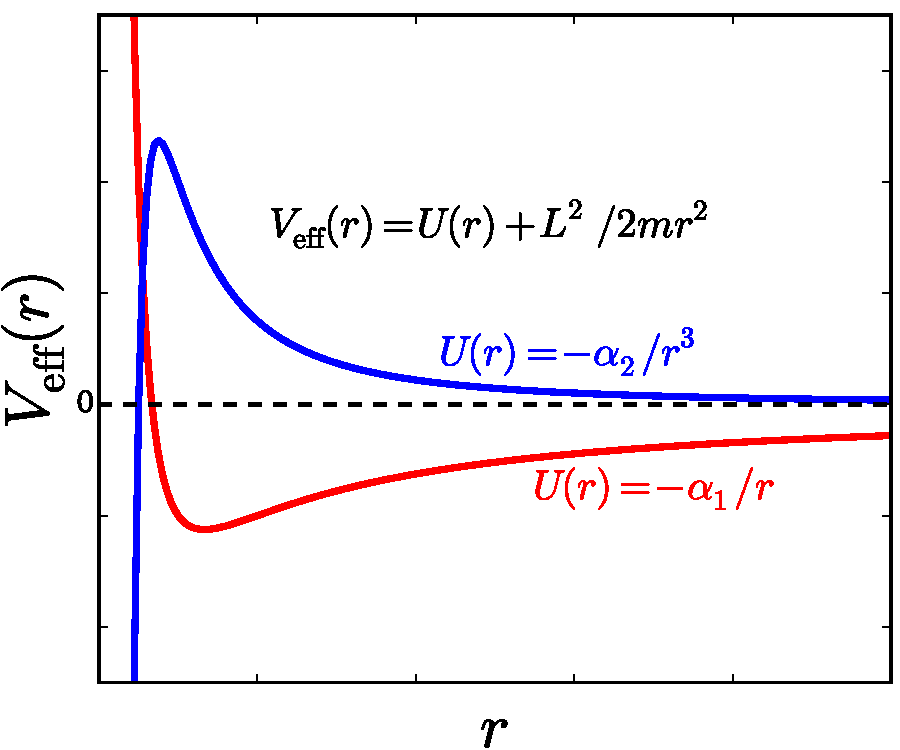
\includegraphics[width=0.45\textwidth]{figs/Veff}}
\caption{\label{fig:Veff}The effective potential is sketched for two cases, a $1/r$ attractive potential and a $1/r^3$ attractive potential. The $1/r$ case has a stable minimum, whereas the circular orbit in the $1/r^3$ case is unstable. 
}
\end{figure}
If one considers a potential that falls as $1/r^3$, the situation is reversed and the point where $\partial_rU$ disappears will be a local maximum rather than a local minimum -- see Fig. \ref{fig:Veff}. The repulsive centrifugal piece dominates at large $r$ and the attractive Coulomb piece wins out at small $r$. The circular orbit is then at a maximum of the effective potential and the orbits are unstable. It is the clear that for potentials that fall as $r^n$, that one must have $n>-2$ for the orbits to be stable.

\example
Consider a potential $U(r)=\beta r$. For a particle of mass $m$ with angular momentum $L$, find the angular frequency of a circular orbit. Then find the angular frequency for small radial perturbations.

{\bf Solution}:\\
For the circular orbit you search for the position $r_{\rm min}$ where the effective potential is minimized,
\begin{eqnarray*}
\partial_r\left\{\beta r+\frac{L^2}{2mr^2}\right\}&=&0,\\
\beta&=&\frac{L^2}{mr_{\rm min}^3},\\
r_{\rm min}&=&\left(\frac{L^2}{\beta m}\right)^{1/3},\\
\dot{\theta}&=&\frac{L}{mr_{\rm min}^2}=\frac{\beta^{2/3}}{(mL)^{1/3}}
\end{eqnarray*}
Now, we can find the angular frequency of small perturbations about the circular orbit. To do this we find the effective spring constant for the effective potential,
\begin{eqnarray*}
k_{\rm eff}&=&\partial_r^2 \left.U_{\rm eff}\right|_{r_{\rm min}}\\
&=&\frac{3L^2}{mr_{\rm min}^4},\\
\omega&=&\sqrt{\frac{k_{\rm eff}}{m}}\\
&=&\frac{\beta^{2/3}}{(mL)^{1/3}}\sqrt{3}.
\end{eqnarray*}
If the two frequencies, $\dot{\theta}$ and $\omega$, differ by an integer factor, the orbit's trajectory will repeat itself each time around. This is the case for the inverse-square force, $\omega=\dot{\theta}$, and for the harmonic oscillator, $\omega=2\dot{\theta}$. In this case, $\omega=\sqrt{3}\dot{\theta}$, and the angles at which the maxima and minima occur change with each orbit.
 
\exampleend

\subsection{Scattering and Cross Sections}

Scattering experiments don't measure entire trajectories. For elastic collisions, they measure the distribution of final scattering angles at best. Most experiments use targets thin enough so that the number of scatterings is typically zero or one. The cross section, $\sigma$, describes the cross-sectional area for particles to scatter with an individual target atom or nucleus. Cross section measurements form the basis for MANY fields of physics. BThe cross section, and the differential cross section, encapsulates everything measurable for a collision where all that is measured is the final state, e.g. the outgoing particle had momentum $\vec{p}_f$. y studying cross sections, one can infer information about the potential interaction between the two particles. Inferring, or constraining, the potential from the cross section is a classic {\it inverse} problem. Collisions are either elastic or inelastic. Elastic collisions are those for which the two bodies are in the same internal state before and after the collision. If the collision excites one of the participants into a higher state, or transforms the particles into different species, or creates additional particles, the collision is inelastic. Here, we consider only elastic collisions.

For Coulomb forces, the cross section is infinite because the range of the Coulomb force is infinite, but for interactions such as the strong interaction in nuclear or particle physics, there is no long-range force and cross-sections are finite. Even for Coulomb forces, the part of the cross section that corresponds to a specific scattering angle, $d\sigma/d\Omega$, which is a function of the scattering angle $\theta_s$ is still finite.

If a particle travels through a thin target, the chance the particle scatters is $P_{\rm scatt}=\sigma dN/dA$, where $dN/dA$ is the number of scattering centers per area the particle encounters. If the density of the target is $\rho$ particles per volume, and if the thickness of the target is $t$, the areal density (number of target scatterers per area) is $dN/dA=\rho t$. Because one wishes to quantify the collisions independently of the target, experimentalists measure scattering probabilities, then divide by the areal density to obtain cross-sections,
\begin{eqnarray}
\sigma=\frac{P_{\rm scatt}}{dN/dA}.
\end{eqnarray}
Instead of merely stating that a particle collided, one can measure the probability the particle scattered by a given angle. The scattering angle $\theta_s$ is defined so that at zero the particle is unscattered and at $\theta_s=\pi$ the particle is scattered directly backward. Scattering angles are often described in the center-of-mass frame, but that is a detail we will neglect for this first discussion, where we will consider the scattering of particles moving classically under the influence of fixed potentials $U(\vec{r})$. Because the distribution of scattering angles can be measured, one expresses the differential cross section,
\begin{equation}
\frac{d^2\sigma}{d\cos\theta_s~d\phi}.
\end{equation}
Usually, the literatures expresses differential cross sections as
\begin{equation}
d\sigma/d\Omega=\frac{d\sigma}{d\cos\theta d\phi}=\frac{1}{2\pi}\frac{d\sigma}{d\cos\theta},
\end{equation}
where the last equivalency is true when the scattering does not depend on the azimuthal angle $\phi$, as is the case for spherically symmetric potentials. 

The differential solid angle $d\Omega$ can be thought of as the area subtended by a measurement, $dA_d$, divided by $r^2$, where $r$ is the distance to the detector,
\begin{eqnarray}
dA_d=r^2 d\Omega.
\end{eqnarray}
With this definition $d\sigma/d\Omega$ is independent of the distance from which one places the detector, or the size of the detector (as long as it is small).

Differential scattering cross sections are calculated by assuming a random distribution of impact parameters $b$. These represent the distance in the $xy$ plane for particles moving in the $z$ direction relative to the scattering center. An impact parameter $b=0$ refers to being aimed directly at the target's center. The impact parameter describes the transverse distance from the $z=0$ axis for the trajectory when it is still far away from the scattering center and has not yet passed it. The differential cross section can be expressed in terms of the impact parameter,
\begin{equation}
d\sigma=2\pi bdb,
\end{equation}
which is the area of a thin ring of radius $b$ and thickness $db$. In classical physics, one can calculate the trajectory given the incoming kinetic energy $E$ and the impact parameter if one knows the mass and potential. From the trajectory, one then finds the scattering angle $\theta_s(b)$. The differential cross section is then
\begin{equation}
\frac{d\sigma}{d\Omega}=\frac{1}{2\pi}\frac{d\sigma}{d\cos\theta_s}=b\frac{db}{d\cos\theta_s}=\frac{b}{(d/db)\cos\theta_s(b)}.
\end{equation}
Typically, one would calculate $\cos\theta_s$ and $(d/db)\cos\theta_s$ as functions of $b$. This is sufficient to plot the differential cross section as a function of $\theta_s$.

The total cross section is 
\begin{equation}
\sigma_{\rm tot}=\int d\Omega\frac{d\sigma}{d\Omega}=2\pi\int d\cos\theta_s~\frac{d\sigma}{d\Omega}. 
\end{equation}
Even if the total cross section is infinite, e.g. Coulomb forces, one can still have a finite differential cross section as we will see later on.

\example
An asteroid of mass $m$ and kinetic energy $E$ approaches a planet of radius $R$ and mass $M$. What is the cross section for the asteroid to impact the planet?

{\bf Solution}:\\
Calculate the maximum impact parameter, $b_{\rm max}$, for which the asteroid will hit the planet. The total cross  section for impact is $\sigma_{\rm impact}=\pi b_{\rm max}^2$. The maximum cross-section can be found with the help of angular momentum conservation. The asteroid's incoming momentum is $p_0=\sqrt{2mE}$ and the angular momentum is $L=p_0b$. If the asteroid just grazes the planet, it is moving with zero radial kinetic energy at impact. Combining energy and angular momentum conservation and having $p_f$ refer to the momentum of the asteroid at a distance $R$,
\begin{eqnarray*}
\frac{p_f^2}{2m}-\frac{GMm}{R}&=&E,\\
p_fR&=&p_0b_{\rm max},
\end{eqnarray*}
allows one to solve for $b_{\rm max}$,
\begin{eqnarray*}
b_{\rm max}&=&R\frac{p_f}{p_0}\\
&=&R\frac{\sqrt{2m(E+GMm/R)}}{\sqrt{2mE}}\\
\sigma_{\rm impact}&=&\pi R^2\frac{E+GMm/R}{E}.
\end{eqnarray*}
\exampleend

\subsection{Center-of-Mass Coordinates}

Thus far, we have considered the trajectory as if the force is centered around a fixed point. For two bodies interacting only with one another, both masses circulate around the center of mass. One might think that solutions would become more complex when both particles move, but we will see here that the problem can be reduced to one with a single body moving according to a fixed force by expressing the trajectories for $\vec{r}_1$ and $\vec{r}_2$ into the center-of-mass coordinate $\vec{R}_{\rm cm}$ and the relative coordinate $\vec{r}$,
\begin{eqnarray}
\vec{R}_{\rm cm}&\equiv&\frac{m_1\vec{r}_1+m_2\vec{r}_2}{m_1+m_2},\\
\nonumber
\vec{r}&\equiv&\vec{r}_1-\vec{r_2}.
\end{eqnarray}
Here, we assume the two particles interact only with one another, so $\vec{F}_{12}=-\vec{F}_{21}$ (where $\vec{F}_{ij}$ is the force on $i$ due to $j$. The equations of motion then become
\begin{eqnarray}
\ddot{\vec{R}}_{\rm cm}&=&\frac{1}{m_1+m_2}\left\{m_1\ddot{\vec{r}}_1+m_2\ddot{\vec{r}}_2\right\}\\
\nonumber
&=&\frac{1}{m_1+m_2}\left\{\vec{F}_{12}+\vec{F}_{21}\right\}=0.\\
\ddot{\vec{r}}&=&\ddot{\vec{r}}_1-\ddot{\vec{r}}_2=\left(\frac{\vec{F}_{12}}{m_1}-\frac{\vec{F}_{21}}{m_2}\right)\\
\nonumber
&=&\left(\frac{1}{m_1}+\frac{1}{m_2}\right)\vec{F}_{12}.
\end{eqnarray}
The first expression simply states that the center of mass coordinate $\vec{R}_{\rm cm}$ moves at a fixed velocity. The second expression can be rewritten in terms of the reduced mass $\mu$.
\begin{eqnarray}
\mu \ddot{\vec{r}}&=&\vec{F}_{12},\\
\frac{1}{\mu}&=&\frac{1}{m_1}+\frac{1}{m_2},~~~~\mu=\frac{m_1m_2}{m_1+m_2}.
\end{eqnarray}
Thus, one can treat the trajectory as a one-body problem where the reduced mass is $\mu$, and a second trivial problem for the center of mass. The reduced mass is especially convenient when one is considering gravitational problems because then
\begin{eqnarray}
\mu \ddot{r}&=&-\frac{Gm_1m_2}{r^2}\hat{r}\\
\nonumber
&=&-\frac{GM\mu}{r^2}\hat{r},~~~M\equiv m_1+m_2.
\end{eqnarray}
For the gravitational problem, the reduced mass then falls out and the trajectory depends only on the total mass $M$.

The kinetic energy and momenta also have analogues in center-of-mass coordinates. The total and relative momenta are
\begin{eqnarray}
\vec{P}&\equiv&\vec{p}_1+\vec{p}_2=M\dot{\vec{R}}_{\rm cm},\\
\nonumber
\vec{q}&\equiv&\mu\dot{\vec{r}}.
\end{eqnarray}
With these definitions, a little algebra shows that the kinetic energy becomes
\begin{eqnarray}
T&=&\frac{1}{2}m_1|\vec{v}_1|^2+\frac{1}{2}m_2|\vec{v}_2|^2\\
\nonumber
&=&\frac{1}{2}M|\dot{\vec{R}}_{\rm cm}|^2
+\frac{1}{2}\mu|\dot{\vec{r}}|^2\\
\nonumber
&=&\frac{P^2}{2M}+\frac{q^2}{2\mu}.
\end{eqnarray}
The standard strategy is to transform into the center of mass frame, then treat the problem as one of a single particle of mass $\mu$ undergoing a force $\vec{F}_{12}$. Scattering angles can also be expressed in this frame, then transformed into the lab frame. In practice, one sees examples in the literature where $d\sigma/d\Omega$ expressed in both the ``center-of-mass'' and in the ``laboratory'' frame. 

\subsection{Rutherford Scattering}

This refers to the calculation of $d\sigma/d\Omega$ due to an inverse square force, $F_{12}=\pm\alpha/r^2$ for repulsive/attractive interaction. Rutherford compared the scattering of $\alpha$ particles ($^4$He nuclei) off of a nucleus and found the scattering angle at which the formula began to fail. This corresponded to the impact parameter for which the trajectories would strike the nucleus. This provided the first measure of the size of the atomic nucleus. At the time, the distribution of the positive charge (the protons) was considered to be just as spread out amongst the atomic volume as the electrons. After Rutherford's experiment, it was clear that the radius of the nucleus tended to be roughly 4 orders of magnitude smaller than that of the atom, which is less than the size of a football relative to Spartan Stadium.

\begin{figure}[!htb]
\centerline{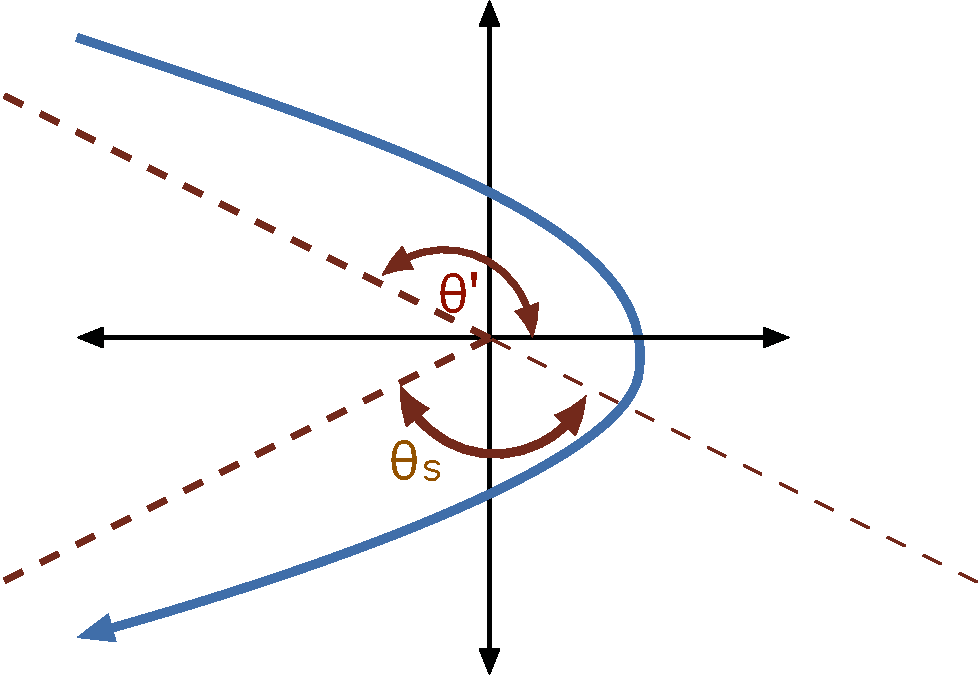
\includegraphics[width=0.6\textwidth]{figs/rutherford}}
\caption{\label{fig:rutherford}
The incoming and outgoing angles of the trajectory are at $\pm\theta'$. They are related to the scattering angle by $2\theta'=\pi+\theta_s$.}
\end{figure}
In order to calculate differential cross section, we must find how the impact parameter is related to the scattering angle. This requires analysis of the trajectory. We consider our previous expression for the trajectory where we derived the elliptic form for the trajectory, Eq. (\ref{eq:Ctrajectory}). For that case we considered an attractive force with the particle's energy being negative, i.e. it was bound. However, the same form will work for positive energy, and repulsive forces can be considered by simple flipping the sign of $\alpha$. For positive energies, the trajectories will be hyperbolas, rather than ellipses, with the asymptotes of the trajectories representing the directions of the incoming and outgoing tracks. Rewriting Eq. (\ref{eq:Ctrajectory}),
\begin{equation}\label{eq:ruthtraj}
r=\frac{1}{\frac{m\alpha}{L^2}+A\cos\theta}.
\end{equation}
Once $A$ is large enough, which will happen when the energy is positive, the denominator will become negative for a range of $\theta$. This is because the scattered particle will never reach certain angles. The asymptotic angles $\theta'$ are those for which the denominator goes to zero,
\begin{equation}
\cos\theta'=-\frac{m\alpha}{AL^2}.
\end{equation}
The trajectory's point of closest approach is at $\theta=0$ and the two angles $\theta'$, which have this value of $\cos\theta'$, are the angles of the incoming and outgoing particles. From Fig. \ref{fig:rutherford}, one can see that the scattering angle $\theta_s$ is given by,
\begin{eqnarray}
\label{eq:sthetover2}
2\theta'-\pi&=&\theta_s,~~~\theta'=\frac{\pi}{2}+\frac{\theta_s}{2},\\
\nonumber
\sin(\theta_s/2)&=&-\cos\theta'\\
\nonumber
&=&\frac{m\alpha}{AL^2}.
\end{eqnarray}
Now that we have $\theta_s$ in terms of $m,\alpha,L$ and $A$, we wish to re-express $L$ and $A$ in terms of the impact parameter $b$ and the energy $E$. This will set us up to calculate the differential cross section, which requires knowing $db/d\theta_s$. It is easy to write the angular momentum as
\begin{equation}
L^2=p_0^2b^2=2mEb^2.
\end{equation}
Finding $A$ is more complicated. To accomplish this we realize that the point of closest approach occurs at $\theta=0$, so from Eq. (\ref{eq:ruthtraj})
\begin{eqnarray}
\label{eq:rminofA}
\frac{1}{r_{\rm min}}&=&\frac{m\alpha}{L^2}+A,\\
\nonumber
A&=&\frac{1}{r_{\rm min}}-\frac{m\alpha}{L^2}.
\end{eqnarray}
Next, $r_{\rm min}$ can be found in terms of the energy because at the point of closest approach the kinetic energy is due purely to the motion perpendicular to $\hat{r}$ and 
\begin{equation}
E=-\frac{\alpha}{r_{\rm min}}+\frac{L^2}{2mr_{\rm min}^2}.
\end{equation}
One can solve the quadratic equation for $1/r_{\rm min}$,
\begin{equation}
\frac{1}{r_{\rm min}}=\frac{m\alpha}{L^2}+\sqrt{(m\alpha/L^2)^2+2mE/L^2}.
\end{equation}
We can plug the expression for $r_{\rm min}$ into the expression for $A$, Eq. (\ref{eq:rminofA}),
\begin{equation}
A=\sqrt{(m\alpha/L^2)^2+2mE/L^2}=\sqrt{(\alpha^2/(4E^2b^4)+1/b^2}
\end{equation}
Finally, we insert the expression for $A$ into that for the scattering angle, Eq. (\ref{eq:sthetover2}),
\begin{eqnarray}
\label{eq:scattangle}
\sin(\theta_s/2)&=&\frac{m\alpha}{AL^2}\\
\nonumber
&=&\frac{a}{\sqrt{a^2+b^2}}, ~~a\equiv \frac{\alpha}{2E}
\end{eqnarray}
The differential cross section can now be found by differentiating the expression for $\theta_s$ with $b$,
\begin{eqnarray}
\label{eq:rutherford}
\frac{1}{2}\cos(\theta_s/2)d\theta_s&=&\frac{ab~db}{(a^2+b^2)^{3/2}}=\frac{bdb}{a^2}\sin^3(\theta_s/2),\\
\nonumber
d\sigma&=&2\pi bdb=\frac{\pi a^2}{\sin^3(\theta_s/2)}\cos(\theta_s/2)d\theta_s\\
\nonumber
&=&\frac{\pi a^2}{2\sin^4(\theta_s/2)}\sin\theta_s d\theta_s\\
\nonumber
\frac{d\sigma}{d\cos\theta_s}&=&\frac{\pi a^2}{2\sin^4(\theta_s/2)},\\
\nonumber
\frac{d\sigma}{d\Omega}&=&\frac{a^2}{4\sin^4(\theta_s/2)}.
\end{eqnarray}
where $a= \alpha/2E$. This the Rutherford formula for the differential cross section. It diverges as $\theta_s\rightarrow 0$ because scatterings with arbitrarily large impact parameters still scatter to arbitrarily small scattering angles. The expression for $d\sigma/d\Omega$ is the same whether the interaction is positive or negative. 

\example
Consider a particle of mass $m$ and charge $z$ with kinetic energy $E$ (Let it be the center-of-mass energy) incident on a heavy nucleus of mass $M$ and charge $Z$ and radius $R$. Find the angle at which the Rutherford scattering formula breaks down.

{\bf Solution}:\\
Let $\alpha=Zze^2/(4\pi\epsilon_0)$. The scattering angle in Eq. (\ref{eq:scattangle}) is 
\[
\sin(\theta_s/2)=\frac{a}{\sqrt{a^2+b^2}}, ~~a\equiv \frac{\alpha}{2E}.
\]
The impact parameter $b$ for which the point of closest approach equals $R$ can be found by using angular momentum conservation,
\begin{eqnarray*}
p_0b&=&b\sqrt{2mE}=Rp_f=R\sqrt{2m(E-\alpha/R)},\\
b&=&R\frac{\sqrt{2m(E-\alpha/R)}}{\sqrt{2mE}}\\
&=&R\sqrt{1-\frac{\alpha}{ER}}.
\end{eqnarray*}
Putting these together
\[
\theta_s=2\sin^{-1}\left\{
\frac{a}{\sqrt{a^2+R^2(1-\alpha/(RE))}}
\right\},~~~a=\frac{\alpha}{2E}.
\]
It was from this departure of the experimentally measured $d\sigma/d\Omega$ from the Rutherford formula that allowed Rutherford to infer the radius of the gold nucleus, $R$.

\exampleend

\subsection{Exercises}

\begin{enumerate}

\item Approximate Earth as a solid sphere of uniform density and radius $R=6360$ km. Suppose you drill a tunnel from the north pole directly to another point on the surface described by a polar angle $\theta$ relative to the north pole. Drop a mass into the hole and let it slide through tunnel without friction. Find the frequency $f$ with which the mass oscillates back and forth. Ignore Earth's rotation. Compare this to the frequency of a low-lying circular orbit.

\item Consider the gravitational field of the moon acting on the Earth.
\begin{enumerate}
\item Calculate the term $k$ in the expansion
\[
g_{\rm moon}=g_0+kz+\cdots,
\]
where $z$ is measured relative to Earth's center and is measured along the axis connecting the Earth and moon. Give your answer in terms of the distance between the moon and the earth, $R_{m}$ and the mass of the moon $M_m$. 
\item Calculate the difference between the height of the oceans at maximum and minimum tides. Express your answer in terms of the quantities above, plus Earth's radius, $R_e$. Then give you answer in meters.
\end{enumerate}

\item Consider an ellipse defined by the sum of the distances from the two foci being $2D$, which expressed in a Cartesian coordinates with the middle of the ellipse being at the origin becomes
\[
\sqrt{(x-a)^2+y^2}+\sqrt{(x+a)^2+y^2}=2D.
\]
Here the two foci are at $(a,0)$ and $(-a,0)$. Show that this form is can be written as
\[
\frac{x^2}{D^2}+\frac{y^2}{D^2-a^2}=1.
\]

\item Consider a particle in an attractive inverse-square potential, $U(r)=-\alpha/r$, where the point of closest approach is $r_{\rm min}$ and the total energy of the particle is $E$. Find the parameter $A$ describing the trajectory in Eq. (\ref{eq:Ctrajectory}). Hint: Use the fact that at $r_{\rm min}$ there is no radial kinetic energy and $E=-\alpha/r_{\rm min}+L^2/2mr_{\rm min}^2$.

\item Consider the effective potential for an attractive inverse-square-law force, $F=-\alpha/r^2$. Consider a particle of mass $m$ with angular momentum $L$.
\begin{enumerate}
\item Find the radius of a circular orbit by solving for the position of the minimum of the effective potential. 
\item What is the angular frequency, $\dot{\theta}$, of the orbit? Solve this by setting $F=m\dot{\theta}^2r$.
\item Find the effective spring constant for the particle at the minimum.
\item What is the angular frequency for small vibrations about the minimum? How does this compare with the answer to (b)?
\end{enumerate}

\item Consider a particle of mass $m$ moving in a potential
\[
U=\alpha\ln(r/a).
\]
\begin{enumerate}
\item If the particle is moving in a circular orbit of radius $R$, find the angular frequency $\dot{\theta}$. Solve this by setting $F=-m\dot{\theta}^2r$ (force and acceleration point inward).
\item Express the angular momentum $L$ in terms of $\alpha$, $m$ and $R$. Also express $R$ in terms of $L$, $\alpha$ and $m$.
\item Sketch the effective radial potential, $V_{\rm eff}(r)$, for a particle with angular momentum $L$. (No longer necessarily moving in a circular orbit.)
\item Find the position of the minimum of $V_{\rm eff}$ in terms of $L$, $\alpha$ and $m$, then compare to the result of (b).
\item What is the effective spring constant for a particle at the minimum of $V_{\rm eff}$? Express your answer in terms of $L$, $m$ and $\alpha$. 
\item What is the angular frequency, $\omega$, for small oscillations of $r$ about the $R_{\rm min}$?  Express your answer in terms of $\dot{\theta}$ from part (a).
\end{enumerate}

\item Consider a particle of mass $m$ in an attractive potential, $U(r)=-\alpha/r$, with angular momentum $L$ with just the right energy so that
\[
A=m\alpha/L^2
\]
where $A$ comes from the expression
\[
r=\frac{1}{(m\alpha/L^2)+A\cos\theta}.
\]
The trajectory can then be rewritten as
\[
r=\frac{2r_0}{1+\cos\theta},~~~r_0=\frac{L^2}{2m\alpha}.
\]
\begin{enumerate}
\item Show that for this case the total energy $E$ approaches zero.
\item Write this trajectory in a more recognizable parabolic form,
\[
x=x_0-\frac{y^2}{R}.
\]
I.e., express $x_0$ and $R$ in terms of $r_0$.
\item Explain how a particle with zero energy can have its trajectory not go through the origin.
\item What is the scattering angle for this trajectory?
\end{enumerate}

\item Show that if one transforms to a reference frame where the total momentum is zero, $\vec{p}_1=-\vec{p}_2$, that the relative momentum $\vec{q}$ corresponds to either $\vec{p}_1$ or $-\vec{p}_2$. This means that in this frame the magnitude of $\vec{q}$ is one half the magnitude of $\vec{p}_1-\vec{p}_2$.

\item Given the center of mass coordinates $\vec{R}$ and $\vec{r}$ for particles of mass $m_1$ and $m_2$, find the coordinates $\vec{r}_1$ and $\vec{r}_2$ in terms of the masses, $\vec{R}$ and $\vec{r}$.

\item Consider two particles of identical mass scattering at an angle $\theta_{\rm cm}$ in the center of mass.
\begin{enumerate}
\item In a frame where one is the target (initially at rest) and one is the projectile, find the scattering angle in the lab frame, $\theta$, in terms of $\theta_{\rm cm}$.
\item Express $d\sigma/d\cos\theta$ in terms of $d\sigma/d\cos\theta_{\rm cm}$. I.e., find the Jacobian, $d\cos\theta_{\rm cm}/d\cos\theta$.
\end{enumerate}

\item Assume you are scattering alpha particles (He-4 nuclei $Z=2, A=4$) off of a gold target ($Z=79, A=197$). If the radius of the nucleus is $7.5\times 10^{-15}$ meters, and if the energy of the beam is 38 MeV,
\begin{enumerate}
\item What is the total cross section for having a nuclear collision? Give the answer in millibarns, 1 mb$=10^{-31}$ m$^2$.
\item Find the scattering angle (in degrees) at which the Rutherford differential cross section formula breaks down?

\end{enumerate}
\end{enumerate}
%\end{document}

\newpage

\setcounter{examplecounter}{0}
% !TEX root = lectures.tex
%% !TEX root =  lectures.tex
\documentclass[12pt]{article}
\usepackage{graphicx}
\usepackage[
	pdfencoding=auto,%
	pdftitle={PHY 321, Classical Mechanics I, Lecture Notes},%
	pdfauthor={Scott Pratt},%
	pdfstartview=FitV,%
	colorlinks=true,%
	linkcolor=blue,%
	citecolor=black, %
	urlcolor=blue]{hyperref}
%\usepackage{pdfsync}
\usepackage{amssymb}
\usepackage{amsmath}
\usepackage{bm}
\usepackage{bbold}
\numberwithin{equation}{section} 
\numberwithin{figure}{section} 
\usepackage[small,bf]{caption}

\usepackage{fontspec}
\usepackage{textcomp}
\usepackage{graphicx}
\usepackage{color}
\usepackage{fancyhdr}
\usepackage{bm}

\newcounter{examplecounter}
\setcounter{examplecounter}{0}
\newcommand{\example}{
\stepcounter{examplecounter}{\nopagebreak\noindent\rule{\textwidth}{1pt}\nopagebreak\\ \bf Example \nopagebreak \arabic{section}.\arabic{examplecounter}:\\ \nopagebreak}}

\newcommand{\exampleend}{
\begin{samepage}
\nopagebreak\noindent\rule{\textwidth}{1pt}
\end{samepage}}

%\usepackage[T1]{fontenc}
%\renewcommand*{\sfdefault}{Berenis}
%\renewcommand*{\rmdefault}{Berenis}
%\renewcommand*{\sfdefault}{phv} % helvetica
%\renewcommand*{\sfdefault}{ppl} % palatino
%\renewcommand*{\rmdefault}{ppl}
%\renewcommand*{\sfdefault}{Bookman}
%\renewcommand*{\rmdefault}{Bookman}

\defaultfontfeatures{Scale=MatchLowercase}
%\setmainfont[Mapping=tex-text,SmallCapsFont={CalifornianFB Expert}]{CalifornianFB}
%\setmainfont[Mapping=tex-text]{Minion Pro}
\setmainfont[Mapping=tex-text]{Palatino Bold}
\setmonofont[Mapping=tex-text]{Courier New Bold}
%\setsansfont[Mapping=tex-text]{Myriad Pro}
%\usepackage{xltxtra}
%\setromanfont{Palatino}
\setromanfont{Palatino Bold}


%\pagestyle{empty}
\textwidth 7.0in
\hoffset -0.8in
\textheight 9.4in
\voffset -1in

\pagestyle{fancy}             % page layout
\newcommand{\TheShortTitle}{}
\newcommand{\ShortTitle}[1]{\renewcommand{\TheShortTitle}{#1}}
\fancyhead[LO,RE]{\slshape \TheShortTitle}
\fancyhead[LE,RO]{\slshape \leftmark}

\usepackage{colortbl}
\newcommand{\cc}[1]{\cellcolor{#1}}
\definecolor{lightred}{rgb}{1,0.5,0.6}
\definecolor{lightblue}{rgb}{0.6,0.8,1.0}

\usepackage{comment}
\parskip 4pt
\parindent 0pt

%\newcommand{\bm}{\boldmath}
\boldmath

% for the banner across the tops of pages 2-
\ShortTitle{PHY 831}

\ShortTitle{PHY 321 Lecture Notes}

\section{Rotating Coordinate Systems}
\bigskip

\subsection{Accelerating Frames}

Here we again consider the effect of uniformly accelerating reference frames. If a particle is observed in an inertial reference frame, which we will denote with a prime, Newton's third law applies
\begin{equation}
m\frac{d^2\vec{r}'}{dt^2}=\vec{F}.
\end{equation}
Now, if we have a second coordinate system,
\begin{equation}
\vec{r}=\vec{r}'-\vec{r}_0,~~~~\vec{r_0}=\frac{1}{2}\vec{a}_0t^2.
\end{equation}
We would see that
\begin{equation}
m\frac{d^2\vec{r}}{dt^2}=\vec{F}-m\vec{a}_0.
\end{equation}
Here $\vec{a}_0$ is the acceleration of the coordinate system. The last term acts like an additional apparent force. In fact, it acts like a contribution to the gravitational force which alters the acceleration of gravity by $\delta\vec{g}=-\vec{a}_0$.

\subsection{Rotating Frames}
If you are on Earth's surface and if your reference frame is fixed with the surface, this is an example of an accelerating frame, where the acceleration is $\omega^2 r_{\perp}$, where $r_{\perp}\equiv\sqrt{x^2+y^2}$, and $\omega$ is the angular velocity of Earth's rotation. The acceleration is inward toward the axis of rotation, so the additional contribution to the apparent acceleration of gravity is outward in the $x-y$ plane. In contrast the usual $\vec{g}$ is radially inward pointing toward the origin. 

In the rotating coordinate system (not an inertial frame), motion is determined by the apparent force and one can define effective potentials. In addition to the normal gravitational potential energy, there is a contribution to the effective potential,
\begin{equation}
\delta U_{\rm eff}=-\frac{m}{2}\omega^2r_\perp^2=-\frac{m}{2}r^2\omega^2\sin^2\theta,
\end{equation}
where $\theta$ is the polar angle, measured from the north pole. If the true gravitational force can be considered as originating from a point in Earth's center, the net effective potential for a mass $m$ near Earth's surface could be 
\begin{equation}
U_{\rm eff}=mgh-m\frac{1}{2}\omega^2(R+h)^2\sin^2\theta.
\end{equation}

\example
How much wider is Earth at the equator than the north-south distance between the poles assuming that the gravitational field above the surface can be approximated by that of a point mass at Earth's center.

{\bf Solution}: 
The surface of the ocean must be at constant effective potential for a sample mass $m$. This means that if $h$ now refers to the height of the water
\[
m g[h(\theta=\pi/2)-h(\theta=0)]=\frac{m}{2}\omega^2(R+h)^2.
\]
Because $R>>h$, one can approximate $R+h\rightarrow R$ on the right-hand side, thus
\[
h(\theta=\pi)-h(\theta=0)=\frac{\omega^2R^2}{2g}.
\]
This come out a bit less than 11 km, or a difference of near 22 km for the diameter of the Earth in the equatorial plane compared to a diameter between the poles. In reality, the difference is approximately 41 km. The discrepancy comes from the assumption that the true gravitational force can be treated as if it came from a point at Earth's center. This would be true if the distribution of mass was radially symmetric. However, Earth's center is molten and the rotation distorts the mass distribution. Remarkably this effect nearly doubles the elliptic distortion of Earth's shape. Due to this distortion, the top of Mount Everest is not the furthest point from the center of the Earth. That belongs to the top of a volcano, Chimborazo, in Equador, which is one degree in latitude below the Equator. Chimborazo is about 8500 ft lower than Everest when measured relative to sea level, but is 7700 feet further from the center of the Earth.

\exampleend

\subsection{Coriolis Force}

Consider some vector $\vec{A}$ according to an observer in a frame rotating about the $z$ axis with angular velocity $\vec{\omega}=\omega\hat{z}$. To an observer in the laboratory frame (the primed frame) the vector will change even if the vector appears fixed to the rotating observer. For a rotation of $\Delta\theta=\omega\Delta t$, the change of the vector due to the rotation is
\begin{eqnarray}
\Delta\vec{A}'=\vec{\omega}\times\vec{A}\Delta t.
\end{eqnarray}
If one includes the fact that $A$, the vector measured in the rotating frame, might be changing as a function of time,
\begin{eqnarray}
\label{eq:dAdtrot}
\Delta\vec{A}'&=&\Delta\vec{A}+\vec{\omega}\times\vec{A}\Delta t,\\
\nonumber
\frac{d}{dt}\vec{A}'&=&\frac{d}{dt}\vec{A}+\vec{\omega}\times\vec{A}.
\end{eqnarray}
If the vector happens to be the position $\vec{r}$,
\begin{eqnarray}
\dot{\vec{r}}'&=&\vec{v}'=\vec{v}+\vec{\omega}\times\vec{r}.
\end{eqnarray}
Here, the first term on the r.h.s. corresponds to the vector $\vec{r}$ not being fixed, but changing with time, $\dot{\vec{r}}=\vec{v}$. One can now use $\vec{v}'=\vec{v}+\vec{\omega}\times\vec{r}$ in place of $\vec{A}$ in Eq. (\ref{eq:dAdtrot}), and see
\begin{eqnarray}
\dot{\vec{v}}'&=&\frac{d}{dt}(\vec{v}+\vec{\omega}\times\vec{r})+\vec{\omega}\times(\vec{v}+\vec{\omega}\times\vec{r})\\
\nonumber
&=&\dot{\vec{v}}+\vec{\omega}\times\dot\vec{r}+\vec{\omega}\times\left(\vec{v}+\vec{\omega}\times\vec{r}\right)\\
\nonumber
&=&\dot{\vec{v}}+2\vec{\omega}\times\vec{v}+\vec{\omega}\times(\vec{\omega}\times\vec{r}).
\end{eqnarray}
Because $\dot{\vec{v}}'$ is $\vec{F}/m$,
\begin{eqnarray}
\label{eq:FmaRotatingFrame}
\vec{F}&=&m\left\{\vec{a}+2\vec{\omega}\times\vec{v}+\vec{\omega}\times(\vec{\omega}\times\vec{r})\right\},\\
\nonumber
m\vec{a}&=&\vec{F}-2m\vec{\omega}\times\vec{v}-m\vec{\omega}\times(\vec{\omega}\times\vec{r}).
\end{eqnarray}
The extra terms on the right behave like additional forces. Like gravitational forces, they are proportional to the mass, so the mass cancels for many problems. 

The last term, $-m\vec{\omega}\times(\vec{\omega}\times\vec{r})$, represents the centrifugal force. Using the vector identity, 
$\vec{A}\times(\vec{B}\times\vec{C})=\vec{B}(\vec{A}\cdot{\vec{C}})-\vec{C}(\vec{A}\cdot\vec{B})$,
\begin{equation}
-\vec{\omega}\times(\vec{\omega}\times\vec{r})=\omega^2\vec{r}+(\omega\cdot\vec{r})\vec{\omega}.
\end{equation}
If $\vec{\omega}$ is in the $z$ direction,
\begin{equation}
-\vec{\omega}\times(\vec{\omega}\times\vec{r})=\omega^2(x\hat{x}+y\hat{y}).
\end{equation}
The centrifugal force points outward in the $x-y$ plane, and its magnitude is $m\omega^2r_{\rm\perp}$, where $r_{\rm\perp}=\sqrt{x^2+y^2}$.

The second term is Eq. (\ref{eq:FmaRotatingFrame}) represents the Coriolis force. It does not enter problems like the shape of the Earth above because in that case the water was not moving relative to the rotating frame. Once an object is moving in a rotating frame, the particle is no longer being described in a single accelerating frame because at each point the acceleration is $-\omega^2\vec{r}$. 

\example
A ball is dropped from a height $h=500$m above Minneapolis. Due to the Coriolis force, it is deflected by an amount $\delta x$ and $\delta y$. Find the deflection. Ignore the centrifugal terms.

{\bf Solution}: The equations of motion are:
\begin{eqnarray*}
\frac{dv_x}{dt}&=&-2(\omega_yv_z-\omega_zv_y),\\
\frac{dv_y}{dt}&=&-2(\omega_zv_x-\omega_xv_z),\\
\frac{dv_z}{dt}&=&-g-2(\omega_xv_y-\omega_yv_x),\\
\omega_z&=&\omega\cos\theta,~~~\omega_y=\omega\sin\theta,~~~\omega_x=0.
\end{eqnarray*}
Here the coordinate system is $\hat{x}$ points east, $\hat{y}$ points north and $\hat{z}$ points upward.

One can now ignore all the Coriolis terms on the right-hand sides except for those with $v_z$. The other terms will all be doubly small. One can also throw out terms with $\omega_x$. This gives
\begin{eqnarray*}
\frac{dv_x}{dt}&\approx& -2\omega v_z\sin\theta,\\
\frac{dv_y}{dt}&\approx& 0,\\
\frac{dv_z}{dt}&\approx& -g.
\end{eqnarray*}
There will be no significant deflection in the $y$ direction, $\delta y=0$, but in the $x$ direction one can substitute $v_z=-gt$ above,
\begin{eqnarray*}
v_x&\approx&\int_0^t dt'~2\omega gt'\sin\theta=\omega gt^2\sin\theta,\\
\delta x&\approx& \int_0^t dt'~v_x(t')=\frac{g\omega\sin\theta t^3}{3}.
\end{eqnarray*}
One can find the deflections by using $h=\frac{1}{2}gt^2$, to find the time, and using the all-knowing internet to see that the latitude of Minneapolis is $44.6^\circ$ or $\theta=45.4^\circ$.
\begin{eqnarray*}
t&=&\sqrt{2h/g}=10.1~{\rm s},\\
\omega&=&\frac{2\pi}{3600\cdot 24~{\rm s}}=7.27\times 10^{-5}~{\rm s}^{-1},\\
\delta x&=&17.4~{\rm cm}~~{\rm(east)}.
\end{eqnarray*}

\exampleend


\subsection{The Foucault Pendulum}
The Foucault Pendulum is simply a regular pendulum moving in both horizontal directions, and with the Coriolis force included. In this case,
\begin{eqnarray*}
m\ddot{\vec{r}}&=&\vec{T}+m\vec{g}-2m\vec{\Omega}\times\vec{v},
\end{eqnarray*}
as the centrifugal force term is absorbed into the definition of $\vec{g}$. The magnitude of the tension, $\vec{T}$, is considered constant because we consider only small oscillations. Then $T\approx mg$, and the components, using $\hat{x},\hat{y}$ to correspond to east and north respectively, are
\begin{eqnarray*}
T_x=-mgx/L,~~~T_y=-mgy/L. 
\end{eqnarray*}
If $\Omega$ is the rotation of the earth, and if $\theta$ is the polar angle, $\pi-$lattitude, 
\begin{eqnarray*}
\ddot{x}&=&-gx/L+2\dot{y}\Omega_z,\\
\ddot{y}&=&-gy/L-2\dot{x}\Omega_z.
\end{eqnarray*}
Here we have used the fact that the oscillations are sufficiently small so we can ignore $v_z$. Using $\omega_0\equiv\sqrt{k/m}$,
\begin{eqnarray*}
\ddot{x}-2\Omega_z\dot{y}+\omega_0^2x&=&0\\
\ddot{y}+2\Omega_z\dot{x}+\omega_0^2y&=&0,
\end{eqnarray*}
where $\Omega_z=|\vec{\Omega}|\cos\theta$, with $\theta$ being the polar angle (zero at the north pole). The terms linear in time derivatives are what make life difficult. This will be solved with a trick. We will incorporate both differential equations into a single complex equation where the first/second are the real/imaginary parts.
\begin{eqnarray*}
\eta\equiv x+iy,\\
\ddot{\eta}+2i\Omega_z\dot{\eta}+\omega_0^2\eta&=&0. 
\end{eqnarray*}

Now, we guess at a form for the solutions, $\eta(t)=e^{-i\alpha t}$, which turns the differential equation into
\begin{eqnarray*}
-\alpha^2+2\Omega_z\alpha+\omega_0^2&=&0,\\
\alpha&=&\Omega_z\pm \sqrt{\Omega_z^2+\omega_0^2},\\
&\approx&\Omega_z\pm \omega_0.
\end{eqnarray*}
The solution with two arbitrary constants is then
\begin{eqnarray*}
\eta&=&e^{-i\Omega_zt}\left[C_1e^{i\omega_0t}+C_2e^{-i\omega_0t}\right].
\end{eqnarray*}
Here, $C_1$ and $C_2$ are complex, so they actually represent four arbitrary numbers. These four numbers should be fixed by the four initial conditions, i.e. $x(t=0), \dot{x}(t=0), y(t=0)$ and $\dot{y}(t=0)$. With some lengthy algebra, one can rewrite the expression as
\begin{eqnarray*}
\label{eq:precmess}
\eta&=&e^{-i\Omega_zt}\left[A\cos(\omega_0t+\phi_A)+iB\cos(\omega_0t+\phi_B)\right].
\end{eqnarray*}
Here, the four coefficients are represented by the two real arbitrary real amplitudes, $A$ and $B$, and two arbitrary phases, $\phi_A$ and $\phi_B$. For an initial condition where $y=0$ at $t=0$, one can see that $B=0$. This then gives
\begin{eqnarray*}
\eta(t)&=&Ae^{-i\Omega_zt}\cos(\omega_0t+\gamma)\\
\nonumber
&=&A\cos\Omega_zt\cos(\omega_0t+\gamma)+iA\sin\Omega_zt\cos(\omega_0t+\gamma).
\end{eqnarray*}
Translating into $x$ and $y$,
\begin{eqnarray}
x&=&A\cos\Omega_zt\cos(\omega_0t+\gamma),\\
\nonumber
y&=&A\sin\Omega_zt\cos(\omega_0t+\gamma).
\end{eqnarray}
Assuming the pendulum's frequency is much higher than Earth's rotational frequency, $\omega_0>>\Omega_z$, one can see that the plane of the pendulum simply precesses with angular velocity $\Omega_z$. This means that in this limit the pendulum oscillates only in the $x$-direction with frequency many times before the phase $\Omega_zt$ becomes noticeable. Eventually, when $\Omega_zt=\pi/2$, the motion is along the $y$-direction. If you were at the north pole, the motion would switch from the $x$-direction to the $y$ direction every 6 hours. Away from the north pole, $\Omega_z\ne|\vec{\Omega}|$ and the precession frequency is less.  At the equator it does not precess at all. If one were to repeat for the solutions where $A=0$ and $B\ne 0$ in Eq. (\ref{eq:precmess}), one would look at motions that started in the $y$-direction, then precessed toward the $-x$ direction. Linear combinations of the two sets of solutions give pendulum motions that resemble ellipses rather than simple back-and-forth motion.

\subsection{Exercises}

\begin{enumerate}

\item Consider a pail of water spinning about a vertical axis at the center of the pail with frequency $\omega$. Find the height of the water (within a constant) as a function the radius $r_\perp$ from the axis of rotation. Use the concept of a centrifugal potential in the rotating frame.

\item A high-speed cannon shoots a projectile with an initial velocity
  of 1000 m/s in the east direction. The cannon is situated in
  Minneapolis (latitude of 45 degrees) The projectile velocity is
  nearly horizontal and it hits the ground after a distance $x=3000$
  m. Find the alteration of the point of impact in the north-south
  ($y$) direction due to the Coriolis force. Assume the effect is
  small so that you can approximate the eastward ($x$) component of
  the velocity as being constant. Be sure to indicate whether the
  deflection is north or south.

\item Someone wishes to use a Foucault pendulum as a crude clock. If the person lives in Minneapolis (latitude of $45^\circ$), how much time will pass between having the pendulum swinging in the east-west direction until it swings in the north-south direction.

\end{enumerate}
%\end{document}

\newpage

\setcounter{examplecounter}{0}
% !TEX root = lectures.tex
%!TEX encoding = UTF-8 Unicode
%% !TEX root =  lectures.tex
\documentclass[12pt]{article}
\usepackage{graphicx}
\usepackage[
	pdfencoding=auto,%
	pdftitle={PHY 321, Classical Mechanics I, Lecture Notes},%
	pdfauthor={Scott Pratt},%
	pdfstartview=FitV,%
	colorlinks=true,%
	linkcolor=blue,%
	citecolor=black, %
	urlcolor=blue]{hyperref}
%\usepackage{pdfsync}
\usepackage{amssymb}
\usepackage{amsmath}
\usepackage{bm}
\usepackage{bbold}
\numberwithin{equation}{section} 
\numberwithin{figure}{section} 
\usepackage[small,bf]{caption}

\usepackage{fontspec}
\usepackage{textcomp}
\usepackage{graphicx}
\usepackage{color}
\usepackage{fancyhdr}
\usepackage{bm}

\newcounter{examplecounter}
\setcounter{examplecounter}{0}
\newcommand{\example}{
\stepcounter{examplecounter}{\nopagebreak\noindent\rule{\textwidth}{1pt}\nopagebreak\\ \bf Example \nopagebreak \arabic{section}.\arabic{examplecounter}:\\ \nopagebreak}}

\newcommand{\exampleend}{
\begin{samepage}
\nopagebreak\noindent\rule{\textwidth}{1pt}
\end{samepage}}

%\usepackage[T1]{fontenc}
%\renewcommand*{\sfdefault}{Berenis}
%\renewcommand*{\rmdefault}{Berenis}
%\renewcommand*{\sfdefault}{phv} % helvetica
%\renewcommand*{\sfdefault}{ppl} % palatino
%\renewcommand*{\rmdefault}{ppl}
%\renewcommand*{\sfdefault}{Bookman}
%\renewcommand*{\rmdefault}{Bookman}

\defaultfontfeatures{Scale=MatchLowercase}
%\setmainfont[Mapping=tex-text,SmallCapsFont={CalifornianFB Expert}]{CalifornianFB}
%\setmainfont[Mapping=tex-text]{Minion Pro}
\setmainfont[Mapping=tex-text]{Palatino Bold}
\setmonofont[Mapping=tex-text]{Courier New Bold}
%\setsansfont[Mapping=tex-text]{Myriad Pro}
%\usepackage{xltxtra}
%\setromanfont{Palatino}
\setromanfont{Palatino Bold}


%\pagestyle{empty}
\textwidth 7.0in
\hoffset -0.8in
\textheight 9.4in
\voffset -1in

\pagestyle{fancy}             % page layout
\newcommand{\TheShortTitle}{}
\newcommand{\ShortTitle}[1]{\renewcommand{\TheShortTitle}{#1}}
\fancyhead[LO,RE]{\slshape \TheShortTitle}
\fancyhead[LE,RO]{\slshape \leftmark}

\usepackage{colortbl}
\newcommand{\cc}[1]{\cellcolor{#1}}
\definecolor{lightred}{rgb}{1,0.5,0.6}
\definecolor{lightblue}{rgb}{0.6,0.8,1.0}

\usepackage{comment}
\parskip 4pt
\parindent 0pt

%\newcommand{\bm}{\boldmath}
\boldmath

% for the banner across the tops of pages 2-
\ShortTitle{PHY 831}

\ShortTitle{PHY 321 Lecture Notes}

\section{Lagrangians and the Calculus of Variations}
\label{sec:lagrangians}
\bigskip

\subsection{Calculus of Variations and the Euler-Lagrange Equation}

The usual minimization problem one faces involves taking a function
$J(y)$, then finding the single value $y$ for which $J$ is either a
maximum or minimum. In multivariate calculus one also learns to solve
problems where you minimize for multiple variables, $J(y_1,y_2,\cdots
y_n)$, and finding the point $(y_1\cdots y_n)$ in $n-$dimensional
space that maximizes or minimizes the function. Here, we consider what
seems to be a much more ambitious problem. Imagine you have a function
$J(y(x),y'(x);x)$, and you wish to find the extrema for an infinite
number of values of $y$, i.e. $y$ at each point $x$. The function $J$
will not only depend on $y$ at each point $x$, but also on the slope
at each point, plus an additional dependence on $x$. Note we are NOT
finding an optimum value of $x$, we are finding the set of optimum
values of $y$ at each point $x$, or equivalently, finding the function
$y(x)$.

One treats the function $y(x)$ as being unknown while minimizing
\[
J=\int_{x_1}^{x_2}dx~f\{y(x),y'(x);x\}.
\]
Thus, we are minimizing $J$ with respect to an infinite number of
values of $y(x_i)$ at points $x_i$. As an additional criteria, we will
assume that $y(x_1)$ and $y(x_2)$ are fixed, and that that we will
only consider variations of $y$ between the boundaries. The dependence
on the derivative, $y'=dy/dx$, is crucial because otherwise the
solution would involve simply finding the one value of $y$ that
minimized $f$, and $y(x)$ would equal a constant if there were no
explicit $x$ dependence. Furthermore, $y$ wouldn't need to be
continuous at the boundary.

The Euler equation is a differential equation for $y(x)$, that when
solved, provides the required solution. For an extrema
\begin{eqnarray}
\delta J&=&\int_{x_1}^{x_2}dx~\left\{ \frac{\partial f}{\partial
  y}\delta y(x)+\frac{\partial f}{\partial y'}\delta y'(x)\right\}=0.
\end{eqnarray}
For ANY small $\delta y(x)$ at any point $x$, the change should be
zero if one is at an optimum function $y(x)$. Integrating the second
term by parts,
\begin{eqnarray}
\delta J&=&\int_{x_1}^{x_2}dx~\left\{ \frac{\partial f}{\partial
  y}-\frac{d}{dx}\left(\frac{\partial f}{\partial
  y'}\right)\right\}\delta y(x)\\ \nonumber &&+\left.\frac{\partial
  f}{\partial y'}\delta y\right|_{x_2}-\left.\frac{\partial
  f}{\partial y'}\delta y\right|_{x_1}\\ \nonumber &=&0.
\end{eqnarray}
Because $y$ is not allowed to vary at the endpoints, $\delta
y(x_1)=\delta y(x_2)=0$, so the middle line can be ignored.  Also,
this relation must hold for ANY $\delta y$, so one can write the Euler
equations (or sometimes called the Euler Lagrange equations)
\begin{equation}
\label{eq:el}
\frac{\partial f}{\partial y}=\frac{d}{dx}\frac{\partial f}{\partial
  y'}.
\end{equation}
This will yield a differential equations for $y$. Combined with the
boundary conditions,
\begin{equation}
y(x_1)=y_1, ~~~y(x_2)=y_2,
\end{equation}
one can now solve the differential equations for $y$. Because $f$ is
only a function of $f'$, not $f''$ or $f'''$, the $d/dx$ in Euler
Lagrange equation can lead to terms involving $f''$, but not
$f'''$. Thus, the equation will be a second-order differential
equation (not a linear equation usually), and the two boundary
conditions are sufficient to determine the entire equation.

\example\label{ex:brachiostone}\noindent Consider a particle
constrained to move along a path (like a bead moving without friction
on a wire) and you need to design a path from $x=y=0$ to some final
point $x_f,y_f$. Assume there is a constant force in the $x$
direction, $F_x=mg$. Design the path so that the time the bead travels
is a minimum.

{\bf Solution:} The net time is
\[
T=\int \frac{d\ell}{v}=\int_0^{x_f}
dx~\frac{\sqrt{1+y'^2}}{\sqrt{2gx}}={\rm minimum}.
\]
Here we made use of the fact that $d\ell=\sqrt{dx^2+dy^2}$ and that
the velocity is determined by $KE=mv^2/2=mgx$. The Euler equations can
be applied if you first define the function as
\begin{eqnarray*}
f(y,y';x)&=&\frac{\sqrt{1+y'^2}}{\sqrt{x}}.
\end{eqnarray*}
The equations are then
\begin{eqnarray*}
\frac{d}{dx}\frac{\partial f}{\partial y'}&=&0.
\end{eqnarray*}
The simplification ensued from $f$ not having any dependence on
$y$. This yields the differential equation
\begin{eqnarray}
\frac{y'}{x^{1/2}(1+y'^2)^{1/2}}&=&(2a)^{-1/2},
\end{eqnarray}
because $\partial f/\partial y'$ must be a constant, which with some
foresight we label $(2a)^{-1/2}$. One can now solve for $y'$,
\begin{eqnarray*}
(y')^2&=&2ax(1+y'^2)\\ \nonumber
  y'&=&\sqrt{\frac{x}{2a-x}},\\ \nonumber y(x)&=&\int_0^x
  dx'~\frac{\sqrt{x'}dx'}{\sqrt{2a-x'}}=\int_0^x
  dx'~\frac{x'dx'}{\sqrt{2ax'-x'^2}}\\ \nonumber
  &=&\frac{1}{2}\int_0^x\frac{(2x'-2a)dx'}{(2ax'-x'^2)^{1/2}}+a\int_0^x\frac{dx'}{\sqrt{2ax'-x'^2}}\\ \nonumber
  &=&\frac{-1}{2}\int_0^{2ax-x^2}\frac{du}{\sqrt{u}}+a\int_0^x\frac{dx'}{\sqrt{a^2-(x'-a)^2}}\\ &=&-\sqrt{2ax-x^2}+a\cos^{-1}(1-x/a).
\end{eqnarray*}
This turns out to be the equation for a {\it cycloid} or a {\it
  brachiostone}. If you rolled a wheel of radius $a$ down the $y$ axis
and followed a point on the rim, it would trace out a cycloid. Here,
the constant $a$ must be chosen to match the boundary condition,
$y_2=y(x_2)$. You can see the textbook for more details, plus you get
a chance to work with cycloids in the exercises at the end of this
chapter.

\exampleend

\subsection{Auxiliary Constraints}

Sometimes an auxiliary constraint is added to the problem (beyond
fixing the end poits $y_1$ and $y_2$). Just ahead, we will work on the
example of a hanging chain. The shape of the curve minimizes the
potential energy, under the constraint of a fixed length of
chain. Before presenting such an example we first review the method of
Lagrange multipliers as a method for finding minima or maxima under
constraints.

Imagine a function $f(x_1,x_2\cdots x_n)$ for which you wish to find
the minima. Additionally, you are given a constraint
\begin{eqnarray}
C(x_1\cdots x_n)=0
\end{eqnarray}
The usual condition for a a minimum is
\begin{eqnarray}
\frac{\partial f}{\partial x_i}=0{\rm ,~~or~}\nabla f=0.
\end{eqnarray}
which would be $n$ equations for the $n$ variables. The gradient of a
scalar is a vector, so you should think of $\nabla$ as
$\vec{\nabla}$. However, the solution will likely not satisfy the
constraint, i.e. the point at which $f(x_1\cdots x_n)$ has an extrema,
may not be a point where $C(x_1\cdots x_n)=0$.

A necessary condition for the solution is that
\begin{equation}
\nabla f\cdot\vec{\epsilon}=0,
\end{equation}
for any infinitesimal vector $\vec{\epsilon}$ if $\vec{\epsilon}$
satisfies the condition
\begin{equation}
\delta C=\nabla C\cdot\vec{\epsilon}=0.
\end{equation}
That is to say if I take a small step in a direction that doesn't
change the constraint, then $f$ must not change if it is an
extrema. Not changing the constraint implies the step is orthogonal to
$\nabla C$. As there are $n$ dimensions of $x$, the vector $\nabla C$
defines one direction, and $\vec{\epsilon}$ can be in any of the $n-1$
directions orthogonal to $\nabla C$. If $\nabla
f\cdot\vec{\epsilon}=0$ for ANY of the $n-1$ directions of
$\vec{\epsilon}$ orthogonal to $\nabla C$, then
\begin{equation}
\nabla f ~||~ \nabla C.
\end{equation}
Because the two vectors are parallel you can say there must exist some
constant $\lambda$ such that
\begin{equation}
\label{eq:lagrangemultiplier}
\nabla(f-\lambda C)=0.
\end{equation}
Here, $\lambda$ is known as a Lagrange multiplier. Satisfying
Eq. (\ref{eq:lagrangemultiplier}) is a necessary, but not a sufficient
condition. One could add a constant to the constraint and the gradient
would not change. One must find the correct value of $\lambda$ that
satisfies the constraint $C=0$, rather than $C=$ some other
constant. The strategy is then to solve
Eq. (\ref{eq:lagrangemultiplier}) then adjust $\lambda$ until one
finds the $x_1\cdots x_n$ that gives $C(x_1\cdots x_n)=0$.

The method of Lagrange multipliers is counter-intuitive to one's
intuition to use the constraint to reduce the dimensionality of the
problem. Normally, minimizing a function of $n$ variables, leads to
$n$ equations and $n$ unknowns. A constraint could be used, by
substitution, to replace the $n$ variables with $n-1$
variables. Instead, we add an unknown parameter, $\lambda$, and change
the equation to $n+1$ equations with $n+1$ unknowns, with the extra
unknown being the Lagrange multiplier $\lambda$. Often, it is rather
easy to solve for $x_1\cdots x_n$. Then one is left with the usually
difficult problem of finding $\lambda$, often requiring the solution
of a transcendental equation.

\example As an example of using Lagrange multipliers for a standard
optimization formula we attempt to maximize the following function,
\[
F(x_1\cdots x_n)=-\sum_{i=1}^n x_i\ln(x_i),
\]
with respect to the $n$ variables $x_i$. With no constraints, each
$x_i$ would maximize the function for
\begin{eqnarray*}
\frac{d}{dx_j}~\left[-\sum_i
  x_i\ln(x_i)\right]&=&0\\ -\ln(x_j)-1&=&0,~~~~x_j=e^{-1}.
\end{eqnarray*}
Now, we repeat the problem but with two constraints,
\[
\sum_ix_i=1~,~~~~\sum_ix_i\epsilon_i=E.
\]
Here, $\epsilon_i$ and $E$ are fixed constants. We go forward by
finding the extrema for
\begin{eqnarray*}
G(x_1\cdots x_n)&=&F-\alpha\sum_i x_i-\beta\sum_i\epsilon_ix_i =\sum_i
\left\{-x_i\ln(x_i)-\alpha x_i-\beta\epsilon_ix_i\right\}.
\end{eqnarray*}
There are two Lagrange multipliers, $\alpha$ and $\beta$,
corresponding to the two constraints. One then solves for the extrema
\begin{eqnarray*}
\frac{d}{dx_j}G&=&0\\ &=&-\ln(x_j)-1-\alpha-\beta\epsilon_j,\\ x_j&=&\exp\left\{-1-\alpha-\beta\epsilon_j\right\}.
\end{eqnarray*}
For any given $\alpha$ and $\beta$ this provides a solution for
constraining $\sum_i x_i$ and $\sum_i\epsilon_ix_i$ to some values,
just not the values of unity and $E$ that you wish. One would then
have to search for the correct values by adjusting $\alpha$ and
$\beta$ until the constraint are actually matched by solving a
transcendental equation. Although this can be complicated, it is
certainly less expensive than searching over all $N$ values of
$x_i$. This particular example corresponds to maximizing the entropy
for a system, $S=-\sum_i x_i\ln(x_i)$, where $x_i$ is the probability
of the system being in a particular discrete level $i$ that has energy
$\epsilon_i$. One wishes to maximize the entropy subject to the
constraints that the probabilities sum to unity and the average energy
has some given value. The result that $x_i\sim e^{-\beta\epsilon_i}$
demonstrates the origin of the Boltzmann factor, with the inverse
temperature $\beta=1/T$.

\exampleend

Lagrange multipliers also assist with the Euler-Lagrange equation. If
one breaks an interval $x_1<x<x_2$ into a large number
$n\rightarrow\infty$ points separated by $dx$, the Euler-Lagrange
equation involves finding the $n$ values $y_i$ at each point so that
$\sum_i dx f\left\{y_i,y'_i=(y_{i+1}-y_{i-1})/(2dx)\right\}$ is
maximized for some given function $f$. If an additional auxiliary
constraint is added, also some function of the $n$ values $y_i$, one
can use the method of Lagrange multipliers. In the constraint can also
be written as some function of $C(y_i,y'_i)$, then one simply adds a
term $\lambda C(y,y')$ to the function $f$ and uses the Euler-Lagrange
equation to find the extrema of.
\begin{eqnarray}
J&=&\int_{x_1}^{x_2}dx~f\left\{y(x),y'(x),x\right\}-\lambda
C\left\{y(x),y'(x),x\right\},
\end{eqnarray}
the one difference being that
\begin{equation}
f\left\{y(x),y'(x),x\right\}\rightarrow
f\left\{y(x),y'(x),x\right\}-\lambda C\left\{y(x),y'(x),x\right\}
\end{equation}
in Eq. (\ref{eq:el}).

\example Consider a chain of length $L$ and mass per unit length
$\kappa$ that hangs from point $x=0,y=0$ to point $x_f,y_f$. The shape
must minimize the potential energy. Find general expressions for the
shape in terms of three constants which must be chosen to match
$y(0)=0, y(x_f)=y_f$ and the fixed length. Equivalently, one finds the
function $y(x)$ that provides an extrema for the integral,

{\bf Solution:} One must minimize
\[
\int d\ell~\kappa gy-\lambda\int d\ell= \int_0^{x_f}
dx~\sqrt{1+y'^2}\kappa gy-\lambda \int_0^{x_f} dx\sqrt{1+y'^2}.
\]
Here $\lambda$ is the Lagrange multiplier associated with constraining
the length of the chain. The constrained length $L$ appears nowhere in
the expression. Instead, one solves for form of the answer, then
adjusts $\lambda$ to give the correct length. For the purposes of the
Euler-Lagrange minimization one considers the function
\begin{eqnarray}
f(y,y';x)&=&\kappa gy\sqrt{1+y'^2}-\lambda\sqrt{1+y'^2}.
\end{eqnarray}
Because $\lambda$ is an unknown constant and because minimizing a
function multiplied by a constant is the same as minimizing the
function, we can equivlently minimize the integral using the function
\begin{eqnarray}
\tilde{f}(y,y';x)&=&y\sqrt{1+y'^2}-\tilde{\lambda}\sqrt{1+y'^2},\\ \nonumber
\tilde{\lambda}&\equiv&\frac{\lambda}{\kappa g}.
\end{eqnarray}
The Euler-Lagrange equations then become
\begin{eqnarray*}
\frac{d}{dx}\left\{
\frac{y'}{\sqrt{1+y'^2}}y-\tilde{\lambda}\frac{y'}{\sqrt{1+y'^2}}
\right\}&=&\sqrt{1+y'^2}.
\end{eqnarray*}
Here, we will guess at the form of the solution,
\begin{eqnarray*}
y'&=&\sinh[(x-x_0)/a],~~y=a\cosh[(x-x_0)/a]+y_0.
\end{eqnarray*}
Plugging into the Euler-Lagange equations,
\begin{eqnarray*}
\frac{d}{dx}\left\{(a\cosh[(x-x_0)/a]+y_0)\frac{\sinh[(x-x_0)/a]}{\cosh[(x-x_0)/a]}-\tilde{\lambda}\frac{\sinh[(x-x_0)/a]}{\cosh[(x-x_0)/a]}\right\}&=&\cosh[(x-x_0)/a],\\ \nonumber
\frac{d}{dx}\left\{(y_0-\tilde{\lambda})\tanh[(x-x_0)/a]\right\}=0.
\end{eqnarray*}
This solution works if $y_0=\tilde{\lambda}$. So the general form of
the solution is
\[
y=\tilde{\lambda}+a\cosh[(x-x_0)/a].
\]
One must find $\tilde{\lambda}$, $x_0$ and $a$ to satisfy three
conditions, $y(x=0)=0$, $y(x=x_f)=y_f$ and that the length is $L$. For
a hanging chain $a$ is positive. A solution with negative $a$ would
represent a maximum of the potential energy. A remarkable property of
the solution is that once you define the length and the end-point
positions $y_1$ and $y_2$, the solution does not depend on $\kappa$ or
$g$. Thus, the shape of the chain would be the same if you took it to
the moon. These solutions are known as {\it
  catenaries},\\ \href{http://en.wikipedia.org/wiki/Catenary}{http://en.wikipedia.org/wiki/Catenary}.

\exampleend

\subsection{Lagrangians}

Lagrangians represent a powerful method for solving problems that
would be nearly impossible by direct application of Newton's third
law, $\vec{F}=m\vec{a}$. The method works well for problems where a
system is well described by a few \textit{generalized coordinates}. A
generalized coordinate might be the angle describing the position of a
pendulum. This one angle takes the place of using $x$ and $y$ to
describe the position of the pendulum, then applying a clumsy
constraint.

The Lagrangian equations of motion can be derived from a principle of
least action, where the action $S$ is defined as
\begin{equation}
S=\int dt~ L(q,\dot{q},t),
\end{equation}
where $q$ is some coordinate that describes the orientation of a
system and the Lagrangian $L$ is defined as
\begin{equation}
L=T-U,
\end{equation}
the difference of the kinetic and potential energies. Minimizing the
action through the Euler-Lagrange equations gives the Lagrangian
equations of motion,
\begin{equation}
\frac{d}{dt}\frac{\partial L}{\partial \dot{q}}=\frac{\partial
  L}{\partial q}.
\end{equation}
We begin with two simple examples, neither of which gains from the
Lagrangian approach.

\example Consider a particle of mass $m$ connected to a spring with
stiffness $k$. Derive the Lagrangian equations of motion.\\ {\bf
  Solution:}
\begin{eqnarray*}
L&=&\frac{1}{2}m\dot{x}^2-\frac{1}{2}kx^2,\\ \frac{d}{dt}\frac{\partial
  L}{\partial \dot{x}}&=&\frac{\partial L}{\partial
  x},\\ m\ddot{x}&=&-kx.
\end{eqnarray*}

\example Derive the Lagrangian equations of motion for a pendulum of
mass $m$ and length $\ell$.
\begin{eqnarray*}
L&=&\frac{m}{2}\ell^2\dot{\theta}^2-mg\ell(1-\cos\theta),\\ \frac{d}{dt}\frac{\partial
  L}{\partial \dot{\theta}}&=&\frac{\partial L}{\partial
  \theta},\\ m\ell^2\ddot{\theta}&=&-mg\ell\sin\theta,\\ \ddot{\theta}&=&-\frac{g}{\ell}\sin\theta,\\ \ddot{\theta}&\approx&-\frac{g}{\ell}\theta.
\end{eqnarray*}
\exampleend

\subsection{Proving Lagrange's Equations of Motion from Newton's Laws}

Lagrange's equations of motion can only be applied for the following
conditions:
\begin{enumerate}
\item The potential energy is a function of the generalized
  coordinates $q_i$, but not of $\dot{q}_i$.
\item The relation between the original coordinates $x,y,z\cdots$ and
  the generalized coordinates does not depend on $\dot{q}_i$,
  e.g. $x(q,t)$ not $x(q,\dot{q},t)$.
\item Any constraints used to reduce the number of degrees of freedom
  are functions of $\vec{q}$, but not of $\dot{\vec{q}}$.
\item The motion is not dissipative (no damping or friction).
\end{enumerate}
Going forward with the proof, consider $x_i(q_1,q_2\cdots,t)$ and look
at the l.h.s. of Lagrange's equations of motion.
\begin{eqnarray}
\label{eq:lagrangederivation1}
\frac{\partial T}{\partial\dot{q}_j}&=&\sum_i\frac{\partial
  T}{\partial\dot{x}_i}\frac{\partial\dot{x}_i}{\partial\dot{q_j}}
+\sum_i\frac{\partial T}{\partial x_i}\frac{\partial
  x_i}{\partial\dot{q_j}}\\ \nonumber &=&\sum_i
m\dot{x}_i\frac{\partial \dot{x}_i}{\partial\dot{q_j}}\\ \nonumber
&=&\sum_i m\dot{x}_i\frac{(\delta x_i/\delta t)|_{{\rm fixed~}q_{j'\ne
      j}}}{\delta q_j/\delta t}\\ \nonumber
&=&\sum_im\dot{x}_i\frac{\delta{x}_i|_{{\rm fixed~}q_{j'\ne
      j}}}{\delta q_j}\\ \nonumber &=&\sum_i m\dot{x}_i\frac{\partial
  x_i}{\partial q_j}.
\end{eqnarray}
In the first line we used the fact that $T$ does not depend on
$x$. Continuing with taking the derivative of $U$,
\begin{eqnarray}
-\frac{\partial U}{\partial\dot{q}_j}&=&-\sum_i\frac{\partial
  U}{\partial x_i}\frac{\partial x_i}{\partial\dot{q}_j}=0.
\end{eqnarray}
In the first line above we used the fact that $U$ does not depend on
$\dot{x}$ then we used the second condition that $x$ does not depend
on $\dot{q}$. Adding the two pieces together, then taking the
derivative w.r.t. time,
\begin{eqnarray}
\nonumber
\frac{d}{dt}\frac{\partial}{\partial\dot{q}}(T-U)&=&\sum_im\ddot{x}_i\frac{\partial
  x_i}{\partial q_j} +\sum_i
m\dot{x}_i\frac{\partial\dot{x}_i}{\partial q_j}.
\end{eqnarray}

Now, we consider the r.h.s. of Lagrange's equations. Because the
kinetic energy depends only on $\dot{x}$ and not $x$, and because the
potential depends on $x$ but not $\dot{x}$,
\begin{eqnarray}
\label{eq:lagrangederivation2}
\frac{\partial}{\partial q_j}(T-U)&=&\sum_i\frac{\partial
  T}{\partial\dot{x}_i}\frac{\partial\dot{x_i}}{\partial q_j}
-\sum_i\frac{\partial U}{\partial x_i}\frac{\partial x_i}{\partial
  q_j}\\ \nonumber &=&\sum_i
m\dot{x}_i\frac{\partial\dot{x_i}}{\partial q_j} -\sum_i\frac{\partial
  U}{\partial x_i}\frac{\partial x_i}{\partial q_j}
\end{eqnarray}
Using the fact that $m\ddot{x}_i=-(\partial/\partial x_i)U$, one can
see that the bottom expressions in Eq.s (\ref{eq:lagrangederivation1})
and (\ref{eq:lagrangederivation2}) are identical,
\begin{equation}
\frac{d}{dt}\frac{\partial}{\partial\dot{q}_i}(T-U)=\frac{\partial}{\partial
  q_i}(T-U).
\end{equation}

\subsection{Lagrangian Examples}

Two examples are presented here. In the first, there are two
generalized coordinates, but the two equations of motion can be
reduced to one through conservation laws (angular momentum in this
case). In the second, there is a time-dependent constraint.

\example Consider a cone of half angle $\alpha$ standing on its tip at
the origin. The surface of the cone is defined as
\[
r=\sqrt{x^2+y^2}=z\tan \alpha.
\]
Find the equations of motion for a particle of mass $m$ moving along
the surface under the influence of a constant gravitational force,
$-mg\hat{z}$. For generalized coordinates use the azimuthal angle
$\phi$ and $r$.

{\bf Solution:}\\ The kinetic energy is
\begin{eqnarray*}
T&=&\frac{1}{2}mr^2\dot{\theta}^2+\frac{1}{2}m(\dot{r}^2+\dot{z}^2)\\ &=&\frac{1}{2}mr^2\dot{\theta}^2+\frac{1}{2}m\dot{r}^2\left(1+\cot^2\alpha\right)\\ &=&\frac{1}{2}mr^2\dot{\theta}^2+\frac{1}{2}m\dot{r}^2\csc^2\alpha.
\end{eqnarray*}
The potential energy is
\[
U=mgr\cot\alpha,
\]
so Lagrange's equations give
\begin{eqnarray*}
\frac{d}{dt}\left(mr^2\dot{\theta}\right)&=&0,\\ \frac{d}{dt}\left(m\csc^2\alpha
\dot{r}\right)&=&mr\dot{\theta}^2-mg\cot\alpha,\\ \ddot{r}&=&r\dot{\theta}^2\sin^2\alpha-g\cos\alpha\sin\alpha
\end{eqnarray*}
The first equation is a statement of the conservation of angular
momentum with $L=mr^2\dot{\theta}$, so the second equation can also be
expressed as
\[
\ddot{r}=\frac{L^2\sin^2\alpha}{m^2r^3}-g\sin\alpha\cos\alpha.
\]

\example A bead slides along a wire bent in the shape of a parabola,
\[
z=\frac{1}{2}kr^2,~~r^2=x^2+y^2.
\]
Also, the parabolic wire is rotating about the $z$ axis with angular
velocity $\omega$. Derive the equations of motion. Are there any
stable configurations?

{\bf Solution:}\\ Using the fact that
\[
\dot{z}=\dot{r}\frac{\partial z}{\partial r}=kr\dot{r},
\]
the kinetic and potential energies are
\begin{eqnarray*}
T&=&\frac{1}{2}m\left(\dot{r}^2+\dot{z}^2+r^2\omega^2\right)\\ &=&\frac{1}{2}m\left(\dot{r}^2+(kr\dot{r})^2+r^2\omega^2\right),\\ U&=&mgkr^2/2.
\end{eqnarray*}
The equations of motion are then
\begin{eqnarray*}
\frac{d}{dt}\left\{m\dot{r}(1+k^2r^2)\right\}&=&-mgkr+mk^2\dot{r}^2r+m\omega^2r,\\ \ddot{r}&=&\frac{-gkr+\omega^2r-k^2\dot{r}^2r}{1+k^2r^2}
\end{eqnarray*}
For a stable configuration, there needs to be a solution with
$\dot{r}=0$ and $\ddot{r}=0$. This can only happen at $r=0$, and then
for the acceleration to be inward for small deviations of $r$ one
needs to have $gk>\omega^2$. If $\omega^2>gk$ the bead will move
outward indefinitely.

\subsection{Small Vibrations and Normal Modes}

Two examples are provided for solving for normal modes. These are
solutions with multiple generalized coordinates, where the motion is
that of simple harmonic motion. However, the motion is only simple for
a particular set of coordinates $q_1$ and $q_2$,
\begin{eqnarray}
q_1&=&A\cos(\omega_1 t),\\ \nonumber q_2&=&B\cos(\omega_2 t),
\end{eqnarray}
while it is not necessarily simple in other coordinates. For example
if $x=q_1+q_2$, and $y=q_1-q_2$, the $x$ and $y$ motions will contain
mixtures of multiple frequencies. For many problems, or in the limit
of small vibrations about a minimum, there is some coordinate system
where the motion is simple. These are normal modes. Characterizing the
normal modes involves finding the frequencies, $\omega_i$, and the
coordinate system where the motion is simple for each coordinate. This
involves finding the direction, or the linear combination of $x_i$
that form the coordinates $q_i$ in which the motion is that of a
single oscillator in each coordinate.

For a first example, we consider a system of springs, where we write
the Lagrangian, then find the normal modes. For the second example, a
double pendulum is considered. In this case, one must first make a
small angle expansion before finding the modes. In principle, problems
could have the same number of normal modes a degrees of freedom. For
example, a system of 7 particles moving in three dimensions has 21
degrees of freedom. However, some of the degrees of freedom do not
have oscillatory behavior. For example, for a rigid body in free
space, the angles describing the orientation evolve, but do not
oscillate. Also, the center-of-mass coordinates of a system of
particles isolated from outside particles moves at constant
velocity. One can also describe these as normal modes, but acknowledge
that their characteristic frequency is zero, as there are no restoring
forces.

\example
\begin{figure}
\centerline{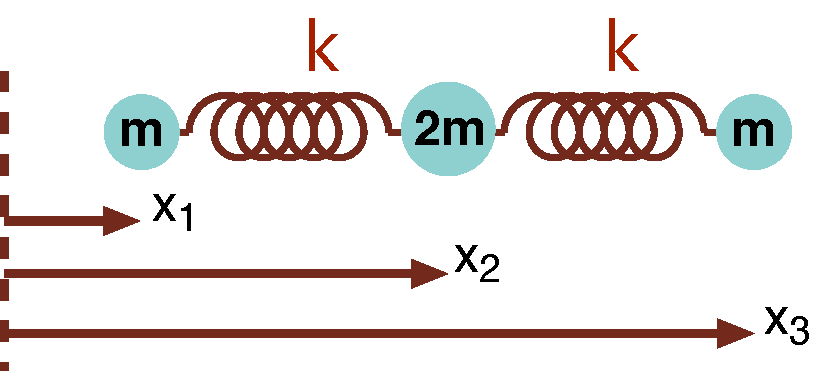
\includegraphics[width=0.5\textwidth]{figs/springs}}
\caption{\label{fig:springs} For Example
  \ref{sec:lagrangians}.\arabic{examplecounter}, three masses
  connected by two springs. The center-of-mass motion is unaffected by
  the springs.}
\end{figure}
Consider two springs, whose relaxed lengths are $\ell$, connected to
three masses as depicted in Fig. \ref{fig:springs}. Describe the two
normal modes of the motion. We can write the Lagrangian as
\begin{eqnarray*}
\mathcal{L}&=&\frac{m}{2}\dot{x}_1^2+m\dot{x}_2^2+\frac{m}{2}\dot{x}_3^2
-\frac{k}{2}(x_2-x_1-\ell)^2-\frac{k}{2}(x_3-x_2-\ell)^2.
\end{eqnarray*}
There are three coordinates, thus there are three equations of motion,
\begin{eqnarray*}
m\ddot{x}_1&=&-k(x_1-x_2+\ell)\\ 2m\ddot{x}_2&=&-k(x_2-x_1-\ell)-k(x_2-x_3+\ell)\\ &=&-k(2x_2-x_1-x_3)\\ m\ddot{x}_3&=&-k(x_3-x_2+\ell).
\end{eqnarray*}
This is a bit complicated because the center-of-mass motion does not
easily separate from the three equations. Instead, choose the
following coordinates,
\begin{eqnarray*}
X&=&\frac{x_1+2x_2+x_3}{4},\\ q_1&=&x_1-x_2+\ell,\\ q_3&=&x_3-x_2-\ell.
\end{eqnarray*}
In these coordinates the potential energy only involves two
coordinates,
\begin{eqnarray*}
U&=&\frac{k}{2}(q_1^2+q_3^2).
\end{eqnarray*}
To express the kinetic energy express $x_1, x_2$ and $x_3$ in terms of
$X$, $q_1$ and $q_3$,
\begin{eqnarray*}
x_1&=&(3q_1-q_3-4\ell+4X)/4,\\ x_2&=&(4X-q_1-q_3)/4,\\ x_3&=&(3q_3-q_1+4\ell+4X)/4.
\end{eqnarray*}
The kinetic energy and Lagrangian are them
\begin{eqnarray*}
T&=&\frac{m}{2}\frac{1}{16}(3\dot{q}_1-\dot{q}_3+4\dot{X})^2
+m\frac{1}{16}(4\dot{X}-\dot{q}_1-\dot{q}_3)^2
+\frac{m}{2}\frac{1}{16}(3\dot{q}_3-\dot{q}_1+4\dot{X})^2\\ &=&\frac{3m}{8}(\dot{q}_1^2+\dot{q}_3^2)-\frac{m}{4}\dot{q}_1\dot{q}_3
+2m\dot{X}^2,\\ \mathcal{L}&=&\frac{3m}{8}(\dot{q}_1^2+\dot{q}_3^2)-\frac{m}{4}\dot{q}_1\dot{q}_3
+2m\dot{X}^2-\frac{k}{2}q_1^2-\frac{k}{2}q_3^2.
\end{eqnarray*}
The three equations of motion are then,
\begin{eqnarray*}
\frac{3}{4}m\ddot{q}_1-\frac{1}{4}m\ddot{q}_3&=&-kq_1,\\ \frac{3}{4}m\ddot{q}_3-\frac{1}{4}m\ddot{q}_1&=&-kq_3,\\ 4M\ddot{X}&=&0.
\end{eqnarray*}
The last equation simply states that the center-of-mass velocity is
fixed. One could obtain the same result by summing the equations of
motion for $x_1$, $2x_2$ and $x_3$ above. The second two equations are
more complicated. To solve them, we assume a form
\begin{eqnarray*}
q_1&=&Ae^{i\omega t},\\ q_3&=&Be^{i\omega t},
\end{eqnarray*}
Because this is a linear equation, we can multiply the solution by a
constant and it will still be a solution. Thus, we can set $B=1$, then
solve for $A$, effectively solving for $A/B$. Putting this guess into
the equations of motion,
\begin{eqnarray*}
-\frac{3}{4}\frac{A}{B}\omega^2+\frac{1}{4}\omega^2&=&-\omega_0^2\frac{A}{B},\\ \frac{3}{4}\omega^2+\frac{1}{4}\frac{A}{B}\omega^2&=&-\omega_0^2.
\end{eqnarray*}
This is two equations and two unknowns, $\omega^2$ and
$A/B$. Substituting for $A/B$ gives a quadratic equation,
\begin{eqnarray*}
\omega^4-3\omega_0^2\omega^2+2\omega_0^4&=&0,\\ \omega_0^2&\equiv&k/m.
\end{eqnarray*}
The two solutions are
\begin{eqnarray*}
(1)~~\omega&=&\omega_0,~~~A=-B,\\ (2)~~\omega&=&\omega_0\sqrt{2},~~~A=B.
\end{eqnarray*}
The first solution corresponds to the two outer masses moving in
opposite directions, in sync, with the middle mass fixed. The second
solution has both outer masses moving in the same direction, but with
the center mass moving opposite. These two solutions are referred to
as normal modes, and are characterized by their frequency and by the
linear combinations of coordinates that oscillate together. In
general, the solution is a linear combination of normal modes, which
usually results in a chaotic looking motion. However, once the
solution is expressed in terms of the normal modes, each of which
oscillates independently in a simple manner, one can better understand
the motion. Further, the frequencies of these modes represent the
natural resonant frequencies of the system. This is important in the
construction of many structures, such as bridges or vehicles.

\example Consider a double pendulum confined to the $x-y$ plane, where
$y$ is vertical. A mass $m$ is connected to the ceiling with a
massless string of length $\ell$. A second mass $m$ hangs from the
first mass with an identical massless string of the same length. Using
$\theta_1$ and $\theta_2$ to describe the orientations of the strings
relative to the vertical axis, find the Lagrangian and derive the
equations of motion, both for arbitrary angles and in the small-angle
approximation. Finally, express the equations of motion in the limit
of small oscillations.

{\bf Solution:}\\ The kinetic and potential energies are:
\begin{eqnarray*}
T&=&\frac{1}{2}m\ell^2\dot{\theta}_1^2
+\frac{1}{2}m\left\{(\ell\dot{\theta}_1\cos\theta_1+\ell\dot{\theta}_2\cos\theta_2)^2
+(\ell\dot{\theta}_1\sin\theta_1+\ell\dot{\theta}_2\sin\theta_2)^2\right\}\\ &=&\frac{1}{2}m\ell^2\left\{2\dot{\theta}_1^2+\dot{\theta}_2^2+2\dot{\theta}_1\dot{\theta}_2\cos(\theta_1-\theta_2)
\right\},\\ U&=&mg\ell(1-\cos\theta_1)+mg\left[\ell(1-\cos\theta_1)+\ell(1-\cos\theta_2)\right]\\ &=&mg\ell(3-2\cos\theta_1-\cos\theta_2)
\end{eqnarray*}
Lagrange's equations for $\theta_1$ lead to
\begin{eqnarray*}
m\ell^2\frac{d}{dt}\left\{2\dot{\theta}_1+\dot{\theta}_2\cos(\theta_1-\theta_2)\right\}&=&
-m\ell^2\dot{\theta}_1\dot{\theta}_2\sin(\theta_1-\theta_2)
-2mg\ell\sin\theta_1,\\ 2\ddot{\theta}_1+\ddot{\theta}_2\cos(\theta_1-\theta_2)+\dot{\theta}_2^2\sin(\theta_1-\theta_2)
&=&-2\omega_0^2\sin\theta_1,\\ \omega_0^2&\equiv& g/\ell,
\end{eqnarray*}
and the equations for $\theta_2$ are
\begin{eqnarray*}
m\ell^2\frac{d}{dt}\left\{\dot{\theta}_2+\dot{\theta}_1\cos(\theta_1-\theta_2)\right\}&=&
m\ell^2\dot{\theta}_1\dot{\theta}_2\sin(\theta_1-\theta_2)-mg\ell\sin\theta_2,\\ \ddot{\theta}_2+\ddot{\theta_1}\cos(\theta_1-\theta_2)&=&
-\omega_0^2\sin\theta_2.
\end{eqnarray*}
For small oscillations, one can only consider terms linear in
$\theta_1$ and $\theta_2$ or their derivatives,
\begin{eqnarray}
\label{eq:doublependulum}
2\ddot{\theta}_1+\ddot{\theta}_2&=&-2\omega_0^2\theta_1,\\ \nonumber
\ddot{\theta}_1+\ddot{\theta}_2&=&-\omega_0^2\theta_2.
\end{eqnarray}
To find the solutions, assume they are of the form
$\theta_1=Ae^{i\omega t}, \theta_2=Be^{i\omega t}$. Solve for $\omega$
and $A/B$, noting that $B$ is arbitrary.

Plug in the desired form and find
\begin{eqnarray*}
e^{i\omega t}(-2\omega^2A-\omega^2B)&=&e^{i\omega
  t}(-2\omega_0^2A),\\ e^{i\omega
  t}(-\omega^2A-\omega^2B)&=&e^{i\omega t}(-\omega_0^2B).
\end{eqnarray*}
We can treat $B$ as arbitrary and set it to unity. When we find $A$,
it is the same as $A/B$ for arbitrary $B$. This gives the equations
\begin{eqnarray*}
2\omega^2A+\omega^2&=&2\omega_0^2A,\\ \omega^2A+\omega^2&=&\omega_0^2.
\end{eqnarray*}
This is two equations and two unknowns. Solving them leads to a
quadratic equation with solutions
\begin{eqnarray*}
A/B&=&\pm\frac{1}{\sqrt{2}},\\ \omega^2&=&\frac{\omega_0^2}{1\pm
  1/\sqrt{2}}.
\end{eqnarray*}
Again, these two solutions are the normal modes, and the general
solution is a sum of the two solutions, with two arbitrary
constants. For the angles $\theta_1$ and $\theta_2$ are:
\begin{eqnarray*}
\theta_1&=&\frac{A_+}{\sqrt{2}}e^{i\omega_+t},
~\theta_2=A_+e^{i\omega_+t},\\ \theta_1&=&\frac{-A_-}{\sqrt{2}}e^{i\omega_-t},
~\theta_2=A_-e^{i\omega_-t},\\ \omega_{\pm}&=&\omega_0\sqrt{\frac{1}{1\pm
    1/\sqrt{2}}}.
\end{eqnarray*}
One can also express the solution in vector notation, with the vectors
having arbitrary amplitudes $A_+$ and $A_-$,
\begin{eqnarray*}
\theta_+&=&\left(\begin{array}{c}
  \frac{1}{\sqrt{2}}\\ 1\end{array}\right)A_+e^{i\omega_+t},\\ \theta_-&=&\left(\begin{array}{c}
    \frac{-1}{\sqrt{2}}\\ 1\end{array}\right)A_-e^{i\omega_-t}.
\end{eqnarray*}
Here, the upper/lower components of the vector describe
$\theta_1/\theta_2$ respectively.

\exampleend

{\bf Aside:} (not applied in this course)\\ These problems can be
treated as linear algebra exercises. Linear algebra is not used in
this course, but nonetheless we describe how this works for the
curious student. In the limit of small vibrations, the equations of
motion can be expressed in the form,
\begin{eqnarray*}
M\ddot{q}&=&-Kq,
\end{eqnarray*}
a form that looks like the spring equation. However, $q$ is an
$n-$dimensional vector and $M$ and $k$ are $n\times n$ matrices. In
the double pendulum example, the dimensionality is 2 and the $q$
refers to the $\theta_1$ and $\theta_2$, and the matrices for $M$ and
$K$ can be read off Eq. (\ref{eq:doublependulum}),
\begin{eqnarray*}
M&=&\left(\begin{array}{cc}
  2&1\\ 1&1\end{array}\right)~,\hspace*{40pt}
  K=\left(\begin{array}{cc}
    2\omega_0^2&0\\ 0&\omega_0^2\end{array}\right).
\end{eqnarray*}
Multiplying both sides of the equation by the inverse matrix $M^{-1}$,
\begin{eqnarray*}
\ddot{q}&=&-\left(M^{-1}K\right)q.
\end{eqnarray*}
Here,
\begin{eqnarray*}
M^{-1}&=&\left(\begin{array}{cc}
  1&-1\\ -1&2\end{array}\right),\\ M^{-1}K&=&\left(\begin{array}{cc}
    2&-1\\ -2&2\end{array}\right)\omega_0^2.
\end{eqnarray*}
One can find a transformation, basically a rotation, that transforms
to a frame where $M^{-1}K$ is diagonal. In this coordinate system the
diagonal components of $M^{-1}K$ represent the squared frequencies of
the normal modes,
\[
M^{-1}K\rightarrow -\left(\begin{array}{cc}
  \omega_+^2&0\\ 0&\omega_-^2\end{array}\right)~,
\]
and are known as ``eigen'' frequencies. The corresponding unit
vectors,
\[
\left(\begin{array}{c} 1\\0\end{array}\right)~{\rm
    and}~\left(\begin{array}{c} 0\\1\end{array}\right)~{\rm
      in~the~new~coordinate~system},
\]
can be rotated back into the original frame, and become the solutions
for the normal modes. These are then called ``eigenvectors'', which
are the same as the normal modes. Finding the eigenfrequencies is
performed by realizing that the determinant of a matrix is unchanged
by the rotation between coordinate systems. Writing the equations of
motion as an eigenvalue problem,
\begin{eqnarray}
\left[A-\lambda_i\mathbb{1}\right]u_i&=&0,~~~A\equiv
M^{-1}K,~\lambda_i\equiv \omega^2_i.
\end{eqnarray}
In the coordinate system where $M^{-1}K$ is diagonal, and the forms
for $u_i$ are simple this requires that in that system, the diagonal
elements of $M^{-1}K$ are the eigenvalues, $\omega_i^2$. For each
$\omega^2_i$, the determinant $|A-\lambda_i\mathbb{1}|$ must
vanish. This is then true in any coordinate system,
\begin{eqnarray}
{\rm det}\left[A-\lambda\mathbb{1}\right]&=&0,
\end{eqnarray}
which for a $2\times 2$ matrix becomes
\begin{eqnarray}
\label{eq:eigen}
\left|
\begin{array}{cc}
A_{11}-\lambda&A_{12}\\ A_{21}&A_{22}-\lambda
\end{array}
\right|&=&0,\\ A_{11}A_{22}-\lambda A_{11}-\lambda
A_{22}+\lambda^2-A_{21}A_{12}&=&0.
\end{eqnarray}
One can solve a quadratic equation for $\lambda$, which gives two
eigenvalues corresponding to $\omega_+^2$ and $\omega_-^2$ found
above. Choosing one of the eigenvalues, one can insert one of the
eigenvalues $\lambda_i$ into Eq. (\ref{eq:eigen}) and solve for $u_i$,
then choose the other eigenvalue and solve for the other corresponding
vector.

If this were a 3-dimensional set of equations, the determinant would
include terms like $\lambda^3$ and would become a cubic equation with
three eigenvalues. One would then solve for three eigenvectors. If one
has a system with dimensionality $n>2$, one usually resorts to solving
the problem numerically due to the messiness of the algebra. The main
programming languages all have packages which readily diagonalize
matrices and find eigenvectors and eigenvalues.
\subsection{Conservation Laws}

Energy is conserved only when the Lagrangian has no explicit
dependence on time, i.e. $L(q,\dot{q})$, not $L(q,\dot{q},t)$. To show
this, we first define the Hamiltonian,
\begin{eqnarray}
\label{eq:Hdef}
H&=&\sum_i\left(\dot{q}_i\frac{\partial
  L}{\partial\dot{q}_i}\right)-L.
\end{eqnarray}
After showing that $H$ is conserved, i.e. $(d/dt)H=0$, we then show
that $H$ can be identified with the total energy, $H=T+V$.

One can see that $H$ is conserved by applying first using the chain
rule for $(d/dt)H$ in Eq. (\ref{eq:Hdef}), then applying Lagrange's
equations,
\begin{eqnarray}
\frac{d}{dt}H&=&\sum_i\left\{\ddot{q}_i\frac{\partial
  L}{\partial\dot{q}_i}+\dot{q}_i\frac{d}{dt}\left(\frac{\partial
  L}{\partial\dot{q}_i}\right)-\frac{\partial
  L}{\partial\dot{q}_i}\ddot{q}_i-\frac{\partial L}{\partial
  q_i}\dot{q}_i\right\}\\ \nonumber
&=&\sum_i\left\{\ddot{q}_i\frac{\partial
  L}{\partial\dot{q}_i}+\dot{q}_i\frac{\partial L}{\partial
  q_i}-\frac{\partial L}{\partial\dot{q}_i}\ddot{q}_i-\frac{\partial
  L}{\partial q_i}\dot{q}_i\right\}\\ \nonumber &=&0.
\end{eqnarray}
These steps assumed that $L$ had no explicit time dependence, i.e. $L$
is a function of $q$ and $\dot{q}$, but not of $t$.

Next, we show that $L$ can be identified with the energy. Because $V$
does not depend on $\dot{q}$,
\begin{equation}
H=\sum_i\frac{\partial T}{\partial\dot{q}_i}\dot{q}_i-T+V.
\end{equation}
If the kinetic energy has a purely quadratic form in terms of
$\dot{q}$,
\begin{equation}
\label{eq:Hquadq}
T=\sum_{ij}A_{ij}(q)\dot{q}_i\dot{q}_j,
\end{equation}
the Hamiltonian becomes
\begin{eqnarray}
H&=&\sum_{ij}2A_{ij}(q)\dot{q}_i\dot{q}_j-\sum_{ij}A_{ij}(q)\dot{q}_i\dot{q}_j+V\\ \nonumber
&=&T+V.
\end{eqnarray}
The proof that $H$ equals the energy hinged on the fact that the
kinetic energy was quadratic in $\dot{q}$. This can be attributed to
time-reversal symmetry. Because the Cartesian coordinates $x_i$ do not
depend on $\dot{q}_i$ or on time, $\dot{x}_i=(\partial x_i/\partial
q_j)\dot{q}_j$. Thus, the kinetic energy, $T=m\dot{x}_i^2/2$, should
be proportional to two powers of $\dot{q}$, which validates the
assumption in Eq. (\ref{eq:Hquadq}).

Here, energy conservation is predicated on the Lagrangian not having
an explicit time dependence. Without an explicit time dependence the
equations of motion are unchanged if one translates a fixed amount in
time because the physics does not depend on when the clock starts. In
contrast, the absolute time becomes relevant if there is an explicit
time dependence. In fact, conservation laws can usually be associated
with symmetries. In this case the translation symmetry in time leads
to energy conservation.

For another example of how symmetry leads to conservation laws,
consider a Lagrangian for a particle of mass $m$ moving in a
two-dimensional plane where the generalized coordinates are the radius
$r$ and the angle $\theta$. The kinetic energy would be
\begin{equation}
T=\frac{1}{2}m\left\{\dot{r}^2+r^2\dot{\theta}^2\right\},
\end{equation}
and if the potential energy $V(r)$ depends only on the radius $r$ and
not on the angle, Lagrange's equations become
\begin{eqnarray}
\frac{d}{dt}(m\dot{r})&=&-\frac{\partial V}{\partial
  r}+m\dot{\theta}^2r,\\ \nonumber \frac{d}{dt}(mr^2\dot{\theta})&=&0.
\end{eqnarray}
The second equation implies that $mr^2\dot{\theta}$ is a
constant. Indeed, it is the angular momentum which is conserved for a
radial force. Here, the conservation of angular momentum is associated
with the independence of the physics to changes in $\theta$, or in
other words, rotational invariance. Once one knows the fact that
$L=mr^2\dot{\theta}$ is conserved, it can be inserted into the
equations of motion for $\dot{r}$,
\begin{equation}
m\ddot{r}=-\frac{\partial V}{\partial r}+\frac{L^2}{mr^3}.
\end{equation}
This is related to Noether's theorem
\href{http://en.wikipedia.org/wiki/Noether's_theorem}{http://en.wikipedia.org/wiki/Noether's\_theorem},
named after Emmy Noether,
\href{http://en.wikipedia.org/wiki/Emmy_Noether}{http://en.wikipedia.org/wiki/Emmy\_Noether}. Simply
stated, if the Lagrangian $L$ is independent of $q_i$, one can see
that the quantity $\partial L/\partial\dot{q}_i$ is conserved,
\begin{equation}
\label{eq:noether}
\frac{d}{dt}\frac{\partial L}{\partial\dot{q}_i}=0.
\end{equation}

Another easy example is in Cartesian coordinates where the potential
depends only on $x$ and $y$ but not on $z$. In that case, there is a
translational symmetry. From Eq. (\ref{eq:noether}), this translates
into conservation of the momentum in the $z$ direction.

\example Consider a pair of particles of mass $m_1$ and $m_2$ where
the potential is of the form
\[
U(\vec{r}_1,\vec{r}_2)=V_a(|m_1\vec{r}_1+m_2\vec{r}_2|/(m_1+m_2))+V_b(|\vec{r}_1-\vec{r}_2|).
\]
Using symmetry arguments alone, are there any conserved components of
the momentum? or the angular momentum??\\

There is no translational invariance, hence there are no conserved
components of the momentum. However, there is rotational invariance
about any axis that goes through the origin. Hence, there is angular
momentum conservation in all three directions. Symmetry arguments are
great ways to recognize the existence of conserved quantities, but
actually expressing them in terms of coordinates can be tricky. For
instance, you may need to write the Lagrangian in terms of angles.

\exampleend

\subsection{Numerically Solving Differential Equations}

Lagrangians lead to equations of motion for the generalized
coordinates. Often, these equations are not analytically solvable, but
are readily addressed computationally. Here, we demonstrate how one
would solve such an equation numerically. So, we first imagine we have
a differential equation for $y(t)$, and for this example we assume the
equation has no derivatives higher than second order. If the boundary
conditions fix $y(0)$ and $y'(0)$, this should be sufficient to
determine $y(t)$ for all future times. Of course, computers need to
discretize the time steps. So assume there are time steps separated by
$\Delta t$ and values,
\begin{eqnarray}
t_n&=&n\Delta t,~=0,\Delta t, 2\Delta t, 3\Delta t\cdots\\ \nonumber
y_n&=&y(t_n).
\end{eqnarray}
Our first step is to solve for $y_{-1}$ and $y_1$ given $y_0$ and
$y'_0$. Approximating the derivatives over the finite intervals,
\begin{eqnarray}
y(0)&=&y_0,\\ \nonumber y'(0)&=&\frac{y_1-y_{-1}}{2\Delta
  t},\\ \nonumber y''(0)&=&\frac{1}{\Delta
  t}\left\{\frac{y_1-y_0}{\Delta t}-\frac{y_0-y_{-1}}{\Delta
  t}\right\} =\frac{y_1-2y_0+y_{-1}}{\Delta t^2}.
\end{eqnarray}
One needs to solve for the three unknowns $y_{-1},y_0$ and
$y_1$. Here, $y(0)$ and $y'(0)$ are given, but $y''(0)$ is not, so a
third equation is needed to solve for the three unknowns. This is
provided by the equations of motion from the Lagrangian. Solving 3
equations and 3 unknowns is thus a fair fight, and one can determine
$y_{-1}\rightarrow y_1$. Once knows these three values, one can use
the differential equation to solve for $y_2$ using $y_0$ and
$y_1$. One can then iteratively find $y_n$ for any $n$ given $y_{n-1}$
and $y_{n-2}$.

\example

Write an algorithm for solving the driven harmonic oscillator,
\[
y''(t)+2\beta y'(t)+\omega_0^2 y(t)=(F_0/m)\cos\omega t.
\]
given $y'(0)=6$ m/s, $y(0)=0.3$ m, and given $m=0.5$ kg, $F_0=400$ N,
and a spring constant $k=2000$ N/m. Let the driving force have a
period of 2.5 s, and the damping rate be $\beta=0.15$ s$^{-1}$.

Let's first solve for $y$ with indices $a,b,c=-1,0,1$, using the
differential equation and the boundary conditions. The BC state that
$y_b=0.3$ m and $(y_c-y_a)=2\Delta t y'_b$, where $y'_b=6$
m/s. Writing the differential equation,
\begin{eqnarray*}
\frac{y_c-2y_b+y_a}{\Delta t^2}+\beta\frac{y_c-y_a}{\Delta
  t}+\omega_0^2 y_b&=&(F_0/m)\cos\omega t_b,
\end{eqnarray*}
one can substitute for $y_a$ because the boundary condition for
$y'_b=y'_0$ gives $y_a=y_{-1}$,
\begin{eqnarray*}
y_a&=&y_c-2\Delta ty'_b,
\end{eqnarray*}
which gives an equation for $y_c$, where everything else in known,
\begin{eqnarray*}
\frac{2y_c-2y_b-2y'_b\Delta t}{\Delta t^2}+2\beta
y'_b+\omega_0^2y_b&=&f_b,\\ \nonumber y_c&=&y_b+y'_b\Delta
t+\left[(f_b/2)-(\omega_0^2y_b/2)-\beta y'_b\right](\Delta t)^2.
\end{eqnarray*}
Here, $f_b\equiv (F_0/m)\cos\omega t$.

Now, that one knows $y_0$ and $y_1$, lets write the differential
equation for three consecutive points $y_a$, $y_b$ and $y_c$, and
solve for $y_c$ in terms of the other two (rather than using the BC as
was done above). Again, beginning with the differential equation,
\begin{eqnarray*}
\frac{y_c-2y_b+y_a}{\Delta t^2}+\beta\frac{y_c-y_a}{\Delta
  t}+\omega_0^2 y_b&=&(F_0/m)\cos\omega
t_b,\\ y_c\left(\frac{1}{\Delta t^2}+\frac{\beta}{\Delta t}\right)
&=&f_b-\omega_0^2y_b+\frac{2y_b-y_a}{\Delta t^2}+\frac{\beta
  y_b}{\Delta
  t},\\ y_c&=&\frac{f_b-\omega_0^2y_b+\frac{2y_b-y_a}{\Delta
    t^2}+\frac{\beta y_b}{\Delta t}}{\frac{1}{\Delta
    t^2}+\frac{\beta}{\Delta t}},\\ &=&\frac{f_b\Delta
  t^2-\omega_0^2y_b\Delta t^2+2y_b-y_a+\beta y_b\Delta
  t}{1+\beta\Delta t}.
\end{eqnarray*}
Using $a=0, b=1, c=2$, this gives $y_2$. Then one can repeat with
$a=1, b=2$ and $c=3$ to find $y_3$, and iterate to find all $n$.

{\bf Solution}:\\ The code might look something like this:
{\tt \begin{verbatim} void main(){ const double PI=4.0*atan(1.0);
    double m=0.5,k=2000.0; double omega0=sqrt(k/m), omega=2.0*PI/2.5,
    beta=0.15; double ya,yb,yc,Dt=0.0025; // Dt = Delta t double
    F0=400,yprime0; // Solve for a,b,c=-1,0,1, solve for yc yb=0.3;
    yprime0=6.0; fb=(F0/m); // Use BC to solve for y_1=yc, from
    lecture notes yc=yb+yprime0*Dt
    +(0.5*fb-0.5*omega0*omega0*yb-beta*yprime0)*Dt*Dt; printf("t=0,
    y=%g\n",yb);
   
   // Now interatively solve for yc, beginning with yc=y_2
   for(n=0;n<1000;n++){ ya=yb; yb=yc; t=(n+1)*Dt;
     fb=(F0/m)*cos(omega*t);
     yc=(fb*Dt^2-omega0^2*yb*Dt*Dt+2*yb-ya+beta*yb*Dt)/(1+beta*Dt);
     printf("t=%g, y=%g\n",Dt*n,yb); } }
\end{verbatim}}
\hrulefill

\subsection{Exercises}

\begin{enumerate}

\item Consider a hill whose height $y$ is given as a function of the
  horizontal coordinate $x$. Consider a segment of the hill from $x=0$
  to $x=L$ with initial height $y(x=0)=0$ and whose final height is
  $y(x=L)=-h$. Transforming the last equation in Example
  \ref{ex:brachiostone} for a downward vertical force rather than a
  horizontal force,
\[
x=-\sqrt{-2ay-y^2}+a\arccos(1+y/a).
\]
Consider a wheel of radius $a$ rolling along the bottom of the $x$
axis. Mark a point on the top of the wheel, which is originally at the
origin, $x=y=0$, when the top of the wheel touches the origin. As the
wheel rolls by an angle $\theta$ the marked point moves due to both
the translation and the rotation of the wheel. The $y$ coordinate of
the marked point is
\[
y=-a(1-\cos\theta),
\]
whereas the $x$ coordinate is
\[
x=a\theta-a\sin\theta.
\]
The first term is due to the horizontal translation of the axis, while
the second term arises from the rotation of the wheel. Re-express
these two equations to find $x(y)$.

\item Consider a chain of length $L$ that hangs from two supports of
  equal height stretched from $x=-X$ to $x=+X$. The general solution
  for a catenary is
\[
y=\lambda+a\cosh[(x-x_0)/a],
\]
\begin{enumerate}
\item Using symmetry arguments, what is $x_0$?
\item Express the length $L$ in terms of $X$ and $a$.
\item Numerically solve the transcendental equation above to find $a$
  in terms of $L=10$ m and $X=4$ m.
\end{enumerate}

\item Consider a mass $m$ connected to a spring with spring constant
  $k$. Rather than being fixed, the other end of the spring oscillates
  with frequency $\omega$ and amplitude $A$. For a generalized
  coordinate, use the displacement of the mass from its relaxed
  position and call it $y=x-\ell-A\cos\omega t$. In this system the
  potential energy of the spring is $ky^2/2$.
\begin{enumerate}
\item Write the kinetic energy in terms of the generalized coordinate.
\item Write down the Lagrangian.
\item Find the equations of motion for $y$.
\end{enumerate}

\item Consider a bead of mass $m$ on a circular wire of radius
  $R$. Assume a force $kx$ acts on the bead, where $x$ and $y$ axes
  run through the center of the circle. Using $\theta$ as the
  generalized coordinate (measured relative to the $x$ axis),
\begin{enumerate}
\item Write the Lagrangian in terms of $\theta$.
\item Find the equations of motion.
\end{enumerate}

\item Consider a pendulum of length $\ell$ with all the mass $m$ at
  its end. The pendulum is allowed to swing freely in both
  directions. Using $\phi$ to describe the azimuthal angle about the
  $z$ axis and $\theta$ to measure the angular deviation of the
  pendulum from the downward direction, address the following
  questions:
\begin{enumerate}
\item If the pendulum is initially moving horizontally with velocity
  $v_0$ and angle $\theta_0=90^\circ$ (horizontal), use energy and
  angular momentum conservation to find the minimum angles of
  $\theta_{\rm min}$ subtended by the pendulum. (Note that the angle
  will oscillate between $90^\circ$ and the minimum angle.
\item Write the Lagrangian using $\theta$ and $\phi$ as generalized
  coordinates.
\item Write the equations of motion for $\theta$ and $\phi$.
\item Rewrite the equations of motion for $\theta$ using angular
  momentum conservation to eliminate and reference to $\phi$.
\item Find the value of $L$ required for the stable orbit to be at
  $\theta=45^\circ$.
\item For the steady orbit found in (e) consider small perturbations
  of the orbit. Find the frequency with which the pendulum oscillates
  around $\theta=45^\circ$.
\end{enumerate}

\item Consider a mass $m$ that is connected to a wall by a spring with
  spring constant $k$. A second identical mass $m$ is connected to the
  first mass by an identical spring. Motion is confined to the $x$
  direction.
\begin{enumerate}
\item Write the Lagrangian in terms of the positions of the two masses
  $x_1$ and $x_2$.
\item Solve for the equations of motion.
\item Find two solutions of the type
\begin{eqnarray*}
x_1&=&Ae^{i\omega t},~~~x_2=Be^{i\omega t}.
\end{eqnarray*}
Solve for $A/B$ and $\omega$. Express your answers in terms of
$\omega_0^2=k/m$.
\end{enumerate}

\item Consider two masses $m_1$ and $m_2$ interacting according to a
  potential $V(\vec{r}_1-\vec{r}_2)$.
\begin{enumerate}
\item Write the Lagrangian in terms of the generalized coordinates
  $\vec{R}_{\rm cm}=(m_1\vec{r}_1+m_2\vec{r}_2)/(m_1+m_2)$ and
  $\vec{r}=\vec{r}_1-\vec{r}_2$, and their derivatives.
\item Using the independence of the Lagrangian with respect to
  $\vec{R}_{\rm cm}$, find expressions for the conserved total
  momentum.
\end{enumerate}

\end{enumerate}
%\end{document}


\end{document}
